% !TeX spellcheck = en_US
%\lstset{style=java,style=featurehouse,style=jml,tabsize=2,escapechar=|,style=scriptsize,frame=none}%style=slides,
\newcommand{\featuremodule}[1]{\hfill#1~~~}

% TODO use resize box to fill code to available width \resizebox{60mm}{!}{}
\lstset{style=java,tabsize=2,escapechar=|,frame=none,style=small,backgroundcolor=,commentstyle=\color{blue}\selectfont}%style=featurehouse,style=jml,style=slides,
\newcommand{\centeredlisting}[1]{
	\begin{center}
		\begin{tikzpicture}[every node/.style={rounded corners,draw,thick,fill=white},listing/.style={inner xsep=4pt,inner ysep=3pt}]
			\node[listing] at (0,0) {\makebox{\usebox{#1}}};
		\end{tikzpicture}
	\end{center}
}

%%%%%%%%%% source code with bugs %%%%%%%%%%

\newsavebox{\edgelexicalerror}
\begin{lrbox}{\edgelexicalerror}
	\begin{lstlisting}
class Node {
}

class Edge {
	Node node, node|\tpkt{a1}´\tpkt{a2}|;
}|\errorunderline{a}|
	\end{lstlisting}
\end{lrbox}

\newsavebox{\edgelexicalerrorfix}
\begin{lrbox}{\edgelexicalerrorfix}
	\begin{lstlisting}
class Node {
}

class Edge {
	Node |\tpkt{a1}|first, second|\tpkt{a2}|;
}|\infounderline{a}|
	\end{lstlisting}
\end{lrbox}

\newsavebox{\edgesyntaxerror}
\begin{lrbox}{\edgesyntaxerror}
	\begin{lstlisting}
class Node {
}

class Edge {
	Node first, second;

	Edge(Node first, Node second|\tpkt{a1}|)|\tpkt{a2}|
		this.first = first;
		this.second = second;
	}
}|\errorunderline{a}|
	\end{lstlisting}
\end{lrbox}

\newsavebox{\edgesyntaxerrorfix}
\begin{lrbox}{\edgesyntaxerrorfix}
	\begin{lstlisting}
class Node {
}

class Edge {
	Node first, second;

	Edge(Node first, Node second|\tpkt{a1}|) {|\tpkt{a2}|
		this.first = first;
		this.second = second;
	}
}|\infounderline{a}|
	\end{lstlisting}
\end{lrbox}

\newsavebox{\edgetypeerror}
\begin{lrbox}{\edgetypeerror}
	\begin{lstlisting}
class Edge {
	Node first, second;
	Edge(Node first, Node second) {
		this.first = first;
		this.second = second;
	}
	public static void main(String[] args) {
		Node a = new Node();
		Node b = new Node();
		Edge e = |\tpkt{a1}|new Edge()|\tpkt{a2}|;
		System.out.println(e);
	}
}|\errorunderline{a}|
\end{lstlisting}
\end{lrbox}

\newsavebox{\edgetypeerrorfix}
\begin{lrbox}{\edgetypeerrorfix}
\begin{lstlisting}
class Edge {
	Node first, second;
	Edge(Node first, Node second) {
		this.first = first;
		this.second = second;
	}
	public static void main(String[] args) {
		Node a = new Node();
		Node b = new Node();
		Edge e = new Edge(|\tpkt{a1}|a,b|\tpkt{a2}|);
		System.out.println(e);
	}
}|\infounderline{a}|
\end{lstlisting}
\end{lrbox}

\newsavebox{\edgeruntimeerror}
\begin{lrbox}{\edgeruntimeerror}
	\begin{lstlisting}
class Edge {
	Node first, second;
	Edge(Node first, Node second) {
		this.first = first;
		this.second = second;
	}
	boolean equals(Edge e) {
		return first.equals(|\tpkt{a1}|e.first|\tpkt{a2}|) && second.equals(e.first);
	}
	public static void main(String[] args) {
		Edge e = new Edge(new Node(), new Node());
		System.out.println(e.equals(null));
	}
}|\errorunderline{a}|
	\end{lstlisting}
\end{lrbox}

% warning: any update of the code below may create inconsistencies with screenshot stored in designbycontract/javadoc.png
\newsavebox{\javadoc}
\begin{lrbox}{\javadoc}
	\begin{lstlisting}
class Edge {
	Node first, second;
	Edge(Node first, Node second) {
		this.first = first;
		this.second = second;
	}
	/** Comparison of edges depending on connected nodes.
	 * @param e edge that is not null
	 * @return true if both edges connect same nodes
	 */
	boolean equals(Edge e) {
		return first.equals(e.first) && second.equals(e.first);
	}
	public static void main(String[] args) {
		Edge e = new Edge(new Node(), new Node());
		System.out.println(e.equals(null));
	}
}
	\end{lstlisting}
\end{lrbox}

\newsavebox{\defensiveprogramming}
\begin{lrbox}{\defensiveprogramming}
	\begin{lstlisting}
class Edge {
	Node first, second;
	Edge(Node first, Node second) {
		this.first = first;
		this.second = second;
	}
	boolean equals(Edge e) {
		|\tpkt{a1}|if (e == null)|\tpkt{a2}|
			|\tpkt{b1}|throw new RuntimeException(|\tpkt{b2}|
				|\tpkt{c1}|"non-null parameter expected");|\tpkt{c2}|
		return first.equals(e.first) && second.equals(e.first);
	}
	public static void main(String[] args) {
		Edge e = new Edge(new Node(), new Node());
		System.out.println(e.equals(null));
	}
}|\infounderline{a,b,c}|
	\end{lstlisting}
\end{lrbox}

\newsavebox{\runtimeassertions}
\begin{lrbox}{\runtimeassertions}
	\begin{lstlisting}
class Edge {
	Node first, second;
	Edge(Node first, Node second) {
		this.first = first;
		this.second = second;
	}
	boolean equals(Edge e) {
		|\tpkt{a1}|assert (e == null) : "non-null parameter expected";|\tpkt{a2}|
		return first.equals(e.first) && second.equals(e.first);
	}
	public static void main(String[] args) {
		Edge e = new Edge(new Node(), new Node());
		System.out.println(e.equals(null));
	}
}|\infounderline{a}|
	\end{lstlisting}
\end{lrbox}

\newsavebox{\unittests}
\begin{lrbox}{\unittests}
	\begin{lstlisting}
class Edge {
	Node first, second;
	Edge(Node first, Node second) {
		this.first = first;
		this.second = second;
	}
	boolean equals(Edge e) {
		return first.equals(e.first) && second.equals(e.first);
	}
}
|\tpkt{d1}|import org.junit.Test;|\tpkt{d2}|
|\tpkt{e1}|public class TEdge {|\tpkt{e2}|
	|\tpkt{c1}|@Test|\tpkt{c2}|
	|\tpkt{f1}|public|\tpkt{f2}| void testEqualsNull() {
		Edge e = new Edge(new Node(), new Node());
		assert !e.equals(|\tpkt{b1}|null|\tpkt{b2}|);
	}
}|\infounderline{c,d,e,f}|
	\end{lstlisting}
\end{lrbox}

\newsavebox{\jml}
\begin{lrbox}{\jml}
	\begin{lstlisting}
class Edge {
	//@ invariant first != null && second != null;
	Node first, second;
	Edge(Node first, Node second) {
		this.first = first;
		this.second = second;
	}
	/*@ requires e != null;
		@ ensures \result <==> first.equals(e.first) &&
		@   second.equals(e.second); @*/
	boolean equals(Edge e) {
		return first.equals(e.first) && second.equals(e.first);
	}
}
	\end{lstlisting}
\end{lrbox}

\newsavebox{\jmlisqrt}
\begin{lrbox}{\jmlisqrt}
	\begin{lstlisting}
/*@ public normal_behavior
	@ requires y >= 0;
	@ assignable \nothing;
	@ ensures 0 <= \result
	@   && \result * \result <= y
	@   && ((0 <= (\result + 1) * (\result + 1))
	@   ==> y < (\result + 1) * (\result + 1));
	@*/
public static int isqrt(int y) {
	return (int) Math.sqrt(y);
}
	\end{lstlisting}
\end{lrbox}

\newsavebox{\edgeruntimeerrorfix}
\begin{lrbox}{\edgeruntimeerrorfix}
	\begin{lstlisting}
class Edge {
	Node first, second;
	Edge(Node first, Node second) {
		this.first = first;
		this.second = second;
	}
	boolean equals(Edge e) {
		return first.equals(e.first) && second.equals(e.first);
	}
	public static void main(String[] args) {
		Edge e = new Edge(new Node(), new Node());
		System.out.println(e.equals(|\tpkt{a1}|e|\tpkt{a2}|));
	}
}|\infounderline{a}|
	\end{lstlisting}
\end{lrbox}

\newsavebox{\edgelogicalerror}
\begin{lrbox}{\edgelogicalerror}
	\begin{lstlisting}
class Edge {
	Node first, second;
	Edge(Node first, Node second) {
		this.first = first;
		this.second = second;
	}
	boolean equals(Edge e) {
		return first.equals(e.first) && second.equals(e.first);
	}
	public static void main(String[] args) {
		Edge e = new Edge(new Node(), new Node());
		System.out.println(e.equals(e));
	}
}
	\end{lstlisting}
\end{lrbox}

\newsavebox{\edgelogicalerrorfix}
\begin{lrbox}{\edgelogicalerrorfix}
	\begin{lstlisting}
class Edge {
	Node first, second;
	Edge(Node first, Node second) {
		this.first = first;
		this.second = second;
	}
	boolean equals(Edge e) {
		return first.equals(e.first) && second.equals(e.|\tpkt{a1}|second|\tpkt{a2}|);
	}
	public static void main(String[] args) {
		Edge e = new Edge(new Node(), new Node());
		System.out.println(e.equals(e));
	}
}|\infounderline{a}|
	\end{lstlisting}
\end{lrbox}

\newsavebox{\codeone}
\begin{lrbox}{\codeone}
\begin{lstlisting}
class Edge {
  Node first, second;
	Edge(Node first, Node second) {
		this.first = first;
		this.second = second;
	}
  boolean |\tpkt{b1}|equals(Edge e)|\tpkt{b2}| {
    return first.equals(e.first) && second.equals(e.first);
  }
	public static void main(String[] args) {
		Node a = new Node();
		Node b = new Node();
		Edge e = new Edge(a, b);
		System.out.println(e.|\tpkt{a1}|equals()|\tpkt{a2}|);
	}
}
\end{lstlisting}
\end{lrbox}

\newsavebox{\bugone}
\begin{lrbox}{\bugone}
\begin{lstlisting}
class Edge {
  Node first, second;
	Edge(Node first, Node second) {
		this.first = first;
		this.second = second;
	}
  boolean |\tpkt{b1}|equals(Edge e)|\tpkt{b2}| {
    return first.equals(e.first) && second.equals(e.first);
  }
	public static void main(String[] args) {
		Node a = new Node();
		Node b = new Node();
		Edge e = new Edge(a, b);
		System.out.println(e.|\tpkt{a1}|equals()|\tpkt{a2}|);
	}
}|\errorunderline{a}\warningunderline{b}|
\end{lstlisting}
\end{lrbox}

\newsavebox{\codetwo}
\begin{lrbox}{\codetwo}
\begin{lstlisting}
class Edge {
  Node first, second;
	Edge(Node first, Node second) {
		this.first = first;
		this.second = second;
	}
  boolean equals(Edge e) {
    return first.equals(|\tpkt{a1}|e.first|\tpkt{a2}|) && second.equals(e.first);
  }
	public static void main(String[] args) {
		Node a = new Node();
		Node b = new Node();
		Edge e = new Edge(a, b);
		System.out.println(e.equals(|\tpkt{b1}|null|\tpkt{b2}|));
	}
}|\infounderline{b}|
\end{lstlisting}
\end{lrbox}

\newsavebox{\bugtwo}
\begin{lrbox}{\bugtwo}
\begin{lstlisting}
class Edge {
  Node first, second;
	Edge(Node first, Node second) {
		this.first = first;
		this.second = second;
	}
  boolean equals(Edge e) {
    return first.equals(|\tpkt{a1}|e.first|\tpkt{a2}|) && second.equals(e.first);
  }
	public static void main(String[] args) {
		Node a = new Node();
		Node b = new Node();
		Edge e = new Edge(a, b);
		System.out.println(e.equals(|\tpkt{b1}|null|\tpkt{b2}|));
	}
}|\errorunderline{a}\warningunderline{b}|
\end{lstlisting}
\end{lrbox}

\newsavebox{\bugtwoagain}
\begin{lrbox}{\bugtwoagain}
\begin{lstlisting}
class Edge {
	Node first, second;
	Edge(Node first, Node second) {
		this.first = first; this.second = second;
	}
	boolean equals(Edge e) {
		return first.equals(|\tpkt{a1}|e.first|\tpkt{a2}|) && second.equals(e.first);
	}
}
|\tpkt{d1}|import org.junit.Test;|\tpkt{d2}|
|\tpkt{e1}|public class TEdge {|\tpkt{e2}|
	|\tpkt{c1}|@Test|\tpkt{c2}|
	|\tpkt{f1}|public|\tpkt{f2}| void test1() {
		Node a = new Node();
		Node b = new Node();
		Edge e = new Edge(a, b);
		System.out.println(e.equals(|\tpkt{b1}|null|\tpkt{b2}|));
	}
}|\errorunderline{a}\warningunderline{b}\infounderline{c,d,e,f}|
\end{lstlisting}
\end{lrbox}

\newsavebox{\codethree}
\begin{lrbox}{\codethree}
\begin{lstlisting}
class Edge {
	Node first, second;
	Edge(Node first, Node second) {
		this.first = first; this.second = second;
	}
	boolean equals(Edge e) {
		return first.equals(|\tpkt{a1}|e.first|\tpkt{a2}|) && second.equals(e.first);
	}
}
|\tpkt{d1}|import org.junit.Test;|\tpkt{d2}|
|\tpkt{e1}|public class TEdge {|\tpkt{e2}|
	|\tpkt{c1}|@Test|\tpkt{c2}|
	|\tpkt{f1}|public|\tpkt{f2}| void test1() {
		Node a = new Node();
		Node b = new Node();
		Edge e = new Edge(a, b);
		System.out.println(e.equals(|\tpkt{b1}|e|\tpkt{b2}|));
	}
}|\infounderline{b}|
\end{lstlisting}
\end{lrbox}

\newsavebox{\bugthree}
\begin{lrbox}{\bugthree}
\begin{lstlisting}
class Node {}
class Edge {
	Node first, second;
	Edge(Node first, Node second) {
		this.first = first; this.second = second;
	}
	boolean equals(Edge e) {
		return first.equals(e.first) && second.equals(e.|\tpkt{a1}|first|\tpkt{a2}|);
	}
}
|\tpkt{d1}|import org.junit.Test;|\tpkt{d2}|
|\tpkt{e1}|public class TEdge {|\tpkt{e2}|
	|\tpkt{c1}|@Test|\tpkt{c2}|
	|\tpkt{f1}|public|\tpkt{f2}| void test1() {
		Node a = new Node();
		Node b = new Node();
		|\tpkt{b1}|System.out.println(new Edge(a, b).equals(new Edge(a, b)));|\tpkt{b2}|
	}
}|\errorunderline{b}\warningunderline{a}|
\end{lstlisting}
\end{lrbox}

\newsavebox{\codefour}
\begin{lrbox}{\codefour}
\begin{lstlisting}
class Node {}
class Edge {
	Node first, second;
	Edge(Node first, Node second) {
		this.first = first; this.second = second;
	}
	boolean equals(Edge e) {
	    return first.equals(e.first) && second.equals(e.|\tpkt{a1}|first|\tpkt{a2}|);
	}
}
|\tpkt{d1}|import org.junit.*;|\tpkt{d2}|
|\tpkt{e1}|public class TEdge {|\tpkt{e2}|
	|\tpkt{c1}|@Test|\tpkt{c2}|
	|\tpkt{f1}|public|\tpkt{f2}| void test1() {
		Node a = new Node();
		Node b = new Node();
		|\tpkt{b1}|Assert.assertTrue|\tpkt{b2}|(new Edge(a, b).equals(new Edge(a, b)));
	}
}|\infounderline{b,d}|
\end{lstlisting}
\end{lrbox}

\newsavebox{\bugfour}
\begin{lrbox}{\bugfour}
	\begin{lstlisting}
class Node {}
class Edge {
	Node first, second;
	Edge(Node first, Node second) {
		this.first = first; this.second = second;
	}
	boolean equals(Edge e) {
		return first.equals(e.first) && second.equals(e.|\tpkt{a1}|first|\tpkt{a2}|);
	}
}
|\tpkt{d1}|import org.junit.*;|\tpkt{d2}|
|\tpkt{e1}|public class TEdge {|\tpkt{e2}|
	|\tpkt{c1}|@Test|\tpkt{c2}|
	|\tpkt{f1}|public|\tpkt{f2}| void test1() {
		Node a = new Node();
		Node b = new Node();
		|\tpkt{b1}|Assert.assertTrue(new Edge(a, b).equals(new Edge(a, b)));|\tpkt{b2}|
	}
}|\warningunderline{a}\errorunderline{b}|
	\end{lstlisting}
\end{lrbox}

\newsavebox{\codefive}
\begin{lrbox}{\codefive}
	\begin{lstlisting}
class Node {}
class Edge {
	Node first, second;
	Edge(Node first, Node second) {
		this.first = first; this.second = second;
	}
	boolean equals(Edge e) {
		return first.equals(e.first) && second.equals(e.|\tpkt{a1}|second|\tpkt{a2}|);
	}
}
|\tpkt{d1}|import org.junit.*;|\tpkt{d2}|
|\tpkt{e1}|public class TEdge {|\tpkt{e2}|
	|\tpkt{c1}|@Test|\tpkt{c2}|
	|\tpkt{f1}|public|\tpkt{f2}| void test1() {
		Node a = new Node();
		Node b = new Node();
		|\tpkt{b1}|Assert.assertTrue|\tpkt{b2}|(new Edge(a, b).equals(new Edge(a, b)));
	}
}|\infounderline{a}|
	\end{lstlisting}
\end{lrbox}

\newsavebox{\dbc}
\begin{lrbox}{\dbc}
\begin{lstlisting}
class Node {}
class Edge {
  //@ invariant first != null && second != null;
  Node first, second;
	Edge(Node first, Node second) {
		this.first = first;
		this.second = second;
	}
  /*@ requires e != null;
    @ ensures \result <==> first.equals(e.first) &&
    @   second.equals(e.second); @*/
  boolean equals(Edge e) {
    return first.equals(e.first) && second.equals(e.first);
  }
	public static void main(String[] args) {
		Node a = new Node();
		Node b = new Node();
		System.out.println(new Edge(a, b).equals(null));
	}
}
\end{lstlisting}
\end{lrbox}

\newsavebox{\callee}
\begin{lrbox}{\callee}
\begin{lstlisting}

boolean equals(Edge e) {
	return first.equals(e.first)
	  && second.equals(e.first);
}
|~|
\end{lstlisting}
\end{lrbox}

\newsavebox{\caller}
\begin{lrbox}{\caller}
\begin{lstlisting}
static void main(String[] args) {
	Node a = new Node();
	Node b = new Node();
	System.out.println(
	  new Edge(a, b).equals(null));
}
\end{lstlisting}
\end{lrbox}

\newsavebox{\blamepre}
\begin{lrbox}{\blamepre}
\begin{lstlisting}
/*@ requires e != null; @*/
\end{lstlisting}
\end{lrbox}

\newsavebox{\blamepost}
\begin{lrbox}{\blamepost}
\begin{lstlisting}
/*@ ensures \result <==>
  @ first.equals(e.first) &&
  @ second.equals(e.second); @*/
\end{lstlisting}
\end{lrbox}

%%%%%%%%%% source code for fop %%%%%%%%%%

\newsavebox{\fopbase}
\begin{lrbox}{\fopbase}
	\begin{minipage}{72mm}
\begin{lstlisting}
class Edge {|\featuremodule{Base}|
  Node first, second;
	Edge(Node first, Node second) {
		this.first = first;
		this.second = second;
	}
  boolean equals(Edge e) {
    return first.equals(e.first) &&
      second.equals(e.second);
  }
[...] }
\end{lstlisting}
	\end{minipage}
\end{lrbox}

\newsavebox{\fopweight}
\begin{lrbox}{\fopweight}
	\begin{minipage}{72mm}
\begin{lstlisting}
class Edge {|\featuremodule{Weighted}|
  Integer weight = 0;
	void setWeight(Integer weight) {
		this.weight = weight;
	}
  boolean equals(Edge e) {
    return original(e) && weight == e.weight;
  }
[...] }
\end{lstlisting}
	\end{minipage}
\end{lrbox}

%%%%%%%%%% source code for plain contracting %%%%%%%%%%

\newsavebox{\pcbase}
\begin{lrbox}{\pcbase}
	\begin{minipage}{72mm}
\begin{lstlisting}
class Edge {|\featuremodule{Base}|
  //@ invariant first != null && second != nulljml;
  Node first, second;
  /*@ requires e != null;|\tpkt{a2}\tpkt{b2}\tpkt{d2}|
    @ ensures \result ==> first.equals(e.first) &&
    @ |~| second.equals(e.second); @*/
  boolean equals(Edge e) {
    return first.equals(e.first) &&
      second.equals(e.second);
  }
[...] }
\end{lstlisting}
	\end{minipage}
\end{lrbox}

\newsavebox{\pcweight}
\begin{lrbox}{\pcweight}
	\begin{minipage}{72mm}
\begin{lstlisting}
class Edge {|\featuremodule{Weighted}|
  Integer weight = 0;
  boolean equals(Edge e) {
    return original(e) && weight == e.weight;
  }
[...] }
\end{lstlisting}
	\end{minipage}
\end{lrbox}

%%%%%%%%%% source code for behavioral subtyping %%%%%%%%%%

\newsavebox{\bhsuper}
\begin{lrbox}{\bhsuper}
	\begin{minipage}{55mm}
\begin{lstlisting}
class Edge {
  //@ invariant first != null && second != null;
  Node first, second;
  /*@ requires e != null;|\tpkt{a2}\tpkt{b2}\tpkt{d2}|
    @ ensures \result ==> first.equals(e.first) &&
    @ |~| second.equals(e.second); @*/
  boolean equals(Edge e) {
    return first.equals(e.first) &&
      second.equals(e.second);
  }
  [...]
}
\end{lstlisting}
	\end{minipage}
\end{lrbox}

\newsavebox{\bhsub}
\begin{lrbox}{\bhsub}
	\begin{minipage}{55mm}
\begin{lstlisting}
class WeightedEdge extends Edge {
  Integer weight = 0;
  /*@ also
    @ requires e != null && weight != null;|\tpkt{c2}\tpkt{e2}|
    @ ensures \result ==> weight == e.weight; @*/
  boolean equals(WeightedEdge e) {
    return super(e) && weight.equals(e.weight);
  }
  [...]
}
\end{lstlisting}
	\end{minipage}
\end{lrbox}

\newsavebox{\bhone}
\begin{lrbox}{\bhone}
	\begin{minipage}{40mm}
\begin{lstlisting}
|\tpkt{a1}|new Edge([...]).equals([...]);
\end{lstlisting}
	\end{minipage}
\end{lrbox}

\newsavebox{\bhtwo}
\begin{lrbox}{\bhtwo}
	\begin{minipage}{40mm}
\begin{lstlisting}
Edge e = new WeightedEdge([...]);
|\tpkt{d1}\tpkt{e1}|e.equals([...]);
\end{lstlisting}
	\end{minipage}
\end{lrbox}

\newsavebox{\bhthree}
\begin{lrbox}{\bhthree}
	\begin{minipage}{40mm}
\begin{lstlisting}
|\tpkt{b1}\tpkt{c1}|new WeightedEdge([...]).equals([...]);
\end{lstlisting}
	\end{minipage}
\end{lrbox}

%%%%%%%%%% source code for explicit contract refinement %%%%%%%%%%

\newsavebox{\ecrbase}
\begin{lrbox}{\ecrbase}
	\begin{minipage}{62mm}
\begin{lstlisting}
class Graph {|\featuremodule{Base}|
  //@ invariant edges != null;
  Collection<Edge> edges;
  /*@ requires e != null;
    @ ensures edges.contains(e); @*/
  void add(Edge e) {
    edges.add(e);
  }
[...] }
\end{lstlisting}
	\end{minipage}
\end{lrbox}

\newsavebox{\ecrmaxoc}
\begin{lrbox}{\ecrmaxoc}
	\begin{minipage}{62mm}
\begin{lstlisting}
class Graph {|\featuremodule{MaxEdges}|
  Integer maxEdges = 10;




  void add(Edge e) {
    if (countEdges() < maxEdges)
		  original(e);
  }
[...] }
\end{lstlisting}
	\end{minipage}
\end{lrbox}

\newsavebox{\ecrmaxco}
\begin{lrbox}{\ecrmaxco}
	\begin{minipage}{62mm}
\begin{lstlisting}
class Graph {|\featuremodule{MaxEdges}|
  Integer maxEdges = 10;
  /*@ requires e != null
	  @ |~| && maxEdges != null;
    @ ensures \old(edges.size()) < maxEdges
		@ |~| ==> edges.contains(e); @*/
  void add(Edge e) {
    if (countEdges() < maxEdges)
		  original(e);
  }
[...] }
\end{lstlisting}
	\end{minipage}
\end{lrbox}

\newsavebox{\ecrmax}
\begin{lrbox}{\ecrmax}
	\begin{minipage}{62mm}
\begin{lstlisting}
class Graph {|\featuremodule{MaxEdges}|
  Integer maxEdges = 10;
  /*@ requires original
	  @ |~| && maxEdges != null;
    @ ensures \old(edges.size()) < maxEdges
		@ |~| ==> original; @*/
  void add(Edge e) {
    if (countEdges() < maxEdges)
		  original(e);
  }
[...] }
\end{lstlisting}
	\end{minipage}
\end{lrbox}

%%%%%%%%%% variability encoding %%%%%%%%%%

\newsavebox{\variables}
\begin{lrbox}{\variables}
	\begin{minipage}{50mm}
\begin{lstlisting}
boolean directed = false;
boolean weighted = false;
boolean optimalConnection = false;
\end{lstlisting}
	\end{minipage}
\end{lrbox}

\newsavebox{\variablesd}
\begin{lrbox}{\variablesd}
	\begin{minipage}{50mm}
\begin{lstlisting}
boolean directed = true;
boolean weighted = false;
boolean optimalConnection = false;
\end{lstlisting}
	\end{minipage}
\end{lrbox}

\newsavebox{\variablesw}
\begin{lrbox}{\variablesw}
	\begin{minipage}{50mm}
\begin{lstlisting}
boolean directed = false;
boolean weighted = true;
boolean optimalConnection = false;
\end{lstlisting}
	\end{minipage}
\end{lrbox}

\newsavebox{\variableso}
\begin{lrbox}{\variableso}
	\begin{minipage}{50mm}
\begin{lstlisting}
boolean directed = true;
boolean weighted = true;
boolean optimalConnection = true;
\end{lstlisting}
	\end{minipage}
\end{lrbox}

%%%%%%%%%% miniatures %%%%%%%%%%

\newsavebox{\contracts}
\begin{lrbox}{\contracts}
	\begin{minipage}{\textwidth}
	\newcommand{\callercolor}{white}
	\newcommand{\calleecolor}{red}
	\vspace{15mm}\hspace{54mm}\begin{tikzpicture}[remember picture,overlay,xscale=3.5,yscale=3,every node/.style={rounded corners,draw,thick},listing/.style={preaction={fill=white},inner xsep=-1pt,inner ysep=-2pt},assumption/.style={shorten <= 2pt,shorten >= 2pt,->,line width=1pt,bend right=60}]
		\node[listing,name=callee,preaction={fill=\calleecolor!25!white,path fading=north,fading angle=15},label=above left:callee] at (-1,0) {\usebox{\callee}};
		\node[listing,name=caller,preaction={fill=\callercolor!25!white,path fading=north,fading angle=15},label=above right:caller] at (1,0) {\usebox{\caller}};
		\path[assumption] (caller) edge node[listing,label=above:precondition] {\usebox{\blamepre}} (callee);
		\path[assumption] (callee) edge node[listing,label=above:postcondition] {\usebox{\blamepost}} (caller);
	\end{tikzpicture}
	\end{minipage}
\end{lrbox}

%\newsavebox{\productline}
%\begin{lrbox}{\productline}
%	\begin{minipage}{\textwidth}
%	\vspace{15mm}\hspace{54mm}\begin{tikzpicture}[remember picture,overlay,xscale=3,yscale=1.6,node/.style={rounded corners,draw,thick,fill=white},gen/.style={->,thick,shorten <= 2pt,shorten >= -2pt},valid/.style={->,gray,dashed,thick,shorten <= 2pt,shorten >= 2pt},conf/.style={node,pos=.7}]
%		\node[node,name=codebase] at (-.7,1.5) {\includegraphics[height=.15\textwidth]{../../../pics/featureide/cd-gpl}};
%		\uncover<1->{\node[name=pgraph] at (-1.5,-1.5) {\pgraph};\draw[gen] (codebase) -- node[conf,name=c] {\config{}} (pgraph);}
%		\uncover<1->{\node[name=pdgraph] at (-.5,-1.5) {\pdgraph};\draw[gen] (codebase) -- node[conf,name=cd] {\config{-d}} (pdgraph);}
%		\uncover<1->{\node[name=pwgraph] at (.5,-1.5) {\pwgraph};\draw[gen] (codebase) -- node[conf,name=cw] {\config{-w}} (pwgraph);}
%		\uncover<1->{\node[name=pograph] at (1.5,-1.5) {~~~\pograph~~~};\draw[gen] (codebase) -- node[conf,name=co] {\config{-dwo}} (pograph);}
%		\uncover<1->{\node[node,name=fm] at (.7,1.5) {\fm};\draw[valid] (fm) -- (c);\draw[valid] (fm) -- (cd);\draw[valid] (fm) -- (cw);\draw[valid] (fm) -- (co);}
%	\end{tikzpicture}
%	\end{minipage}
%\end{lrbox}
%
%\newsavebox{\foc}
%\begin{lrbox}{\foc}
%	\begin{minipage}{\textwidth}
%		\vspace{10mm}\hspace{54mm}\begin{tikzpicture}[remember picture,overlay,xscale=6,yscale=1.5,every node/.style={rounded corners,draw,thick,preaction={fill=white}},mechanism/.style={anchor=east},used/.style={shorten <= 2pt,shorten >= 2pt,->,line width=1pt}]
%			\node at (0,0) {\includegraphics[width=\textwidth]{../../../pics/featureide/cd-gpl-contracts.pdf}};
%			\node[name=ecr,mechanism,preaction={fill=blue!25!white,path fading=north,fading angle=15}] at (1,-2) {Explicit contract refinement};
%			\uncover<1->{\node[name=pc,mechanism,preaction={fill=orange!25!white,path fading=north,fading angle=15}] at (1,0) {Plain contracting};
%			\node[name=bs,mechanism,preaction={fill=green!25!white,path fading=north,fading angle=15}] at (1,-1) {Behavioral subtyping};
%			\path[used] (pc) edge (.2,.7);
%			\path[used] (pc) edge (.7,.8);
%			\path[used] (bs) edge (.1,.1);
%			\path[used] (bs) edge (-.5,.9);
%			\path[used] (bs) edge (-.4,-.5);
%			\path[used] (ecr) edge (-.3,-1.2);
%			\path[used] (ecr) edge (-.35,-.3);}
%		\end{tikzpicture}
%	\end{minipage}
%\end{lrbox}
%
%\newsavebox{\proofcomp}
%\begin{lrbox}{\proofcomp}
%	\begin{minipage}{\textwidth}
%		\vspace{0mm}\hspace{54mm}\begin{tikzpicture}[remember picture,overlay,xscale=3,yscale=.8,node/.style={rounded corners,draw,thick,fill=white},gen/.style={->,thick,shorten <= 2pt,shorten >= -2pt},neg/.style={->,thick,shorten <= -2pt,shorten >= 2pt},do/.style={gen,shorten >= 2pt,dashed},label/.style={preaction={fill=white,opacity=.66}}]
%			\node[node,name=codebase] at (-.7,1.5) {\includegraphics[height=.15\textwidth]{../../../pics/featureide/cd-gpl}};
%			\node[label] at (-.7,1.5) {+ partial proofs};
%			\node[name=pgraph] at (-1.5,-1.5) {\pgraph};\draw[gen] (codebase) -- (pgraph);
%			\node[name=pdgraph] at (-.5,-1.5) {\pdgraph};\draw[gen] (codebase) -- (pdgraph);
%			\node[name=pwgraph] at (.5,-1.5) {\pwgraph};\draw[gen] (codebase) -- (pwgraph);
%			\node[name=pograph] at (1.5,-1.5) {\pograph};\draw[gen] (codebase) -- (pograph);
%			\node[label] at (-1.5,-1.5) {+ proofs};
%			\node[label] at (-.5,-1.5) {+ proofs};
%			\node[label] at (.5,-1.5) {+ proofs};
%			\node[label] at (1.5,-1.5) {+ proofs};
%			\node[node,name=pgraphx,align=center] at (-1.5,-4) {theorems\\+ proofs};\draw[neg] (pgraph) -- (pgraphx);
%			\node[node,name=pdgraphx,align=center] at (-.5,-4) {theorems\\+ proofs};\draw[neg] (pdgraph) -- (pdgraphx);
%			\node[node,name=pwgraphx,align=center] at (.5,-4) {theorems\\+ proofs};\draw[neg] (pwgraph) -- (pwgraphx);
%			\node[node,name=pographx,align=center] at (1.5,-4) {theorems\\+ proofs};\draw[neg] (pograph) -- (pographx);
%			\node[name=pgraphz] at (-1.25,-5) {\richtig};
%			\node[name=pdgraphz] at (-.25,-5) {\richtig};
%			\node[name=pwgraphz] at (.75,-5) {\falsch};
%			\node[name=pographz] at (1.75,-5) {\richtig};
%		\end{tikzpicture}
%	\end{minipage}
%\end{lrbox}
%
%\newsavebox{\varenc}
%\begin{lrbox}{\varenc}
%	\begin{minipage}{\textwidth}
%		\vspace{5mm}\hspace{54mm}\begin{tikzpicture}[remember picture,overlay,xscale=3,yscale=1.6,node/.style={rounded corners,draw,thick,fill=white},gen/.style={->,thick,shorten <= 2pt,shorten >= -2pt},conf/.style={node,pos=.5},listing/.style={node,inner xsep=-1pt,inner ysep=-2pt}]
%			\node[node,name=codebase] at (0,1.5) {\includegraphics[height=.15\textwidth]{../../../pics/featureide/cd-gpl}};
%			\node[name=simulator,label=below:metaproduct] at (-1.5,-1.5) {\pmeta};\draw[gen] (codebase) -- node[conf,name=fm] {\fm} (simulator);
%			\node[name=product,label=below:product] at (1.5,-1.5) {\pwgraph};\draw[gen] (codebase) -- node[conf,name=cw] {\config{-w}} (product);
%			\draw[->,green,dashed,thick,shorten <= 2pt,shorten >= 2pt] (simulator) -- node[listing,label=below:product simulation] {\usebox{\variablesw}} (product);
%		\end{tikzpicture}
%	\end{minipage}
%\end{lrbox}
%


% TODO L05 Compilation

\ifuniversity{tubs}{\date{May 12, 2025}}

\author{Thomas Thüm}
\lecture{Compilation}{compilation}

\section{Fundamentals on Compilation}
\subsection{Programming Languages}
\begin{frame}{And the 2020 Turing Award Goes To \ldots\ \mytitlesource{\href{https://awards.acm.org/about/2020-turing}{awards.acm.org}}}
	\begin{fancycolumns}[animation=none]
		\uncover<2->{
			\pic[width=.485\linewidth,trim=45 2 45 2,clip]{people/alfred-v-aho}\hfill
			\pic[width=.485\linewidth,trim=2 2 2 2,clip]{people/jeffrey-d-ullman}
			
			Alfred V.\ Aho \hfill Jeffrey D. Ullman%
		}%
		\nextcolumn
		\uncover<3>{
			\pic[width=.485\linewidth]{books/aho-hopcroft-ullman-design-and-analysis-of-computer-algorithms}\hfill
			\pic[width=.485\linewidth]{books/aho-ullman-principles-of-compiler-design}
			
			1974 \hfill \mycite{Dragon Book}, 1977%
		}%
	\end{fancycolumns}
\end{frame}

\begin{frame}<2>{Recap: Programming Languages Today}
	\slideProgrammingLanguagesToday
\end{frame}

\begin{frame}{Recap: Popularity of Programming Languages}
	\slideTiobeDiagram
\end{frame}

\subsection{Compilation, Interpretation, and Performance}
\begin{frame}{Compilation vs Interpretation}
	\begin{fancycolumns}[T]
		\begin{definition}{Compilation}
			\begin{itemize}
				\item C/C++/Go/Rust/Swift to machine code
				\item Java/Groovy/Kotlin/Scala/Clojure to Java bytecode
			\end{itemize}
		\end{definition}
		\vspace{6mm}
		\begin{center}
			\figCompiler
		\end{center}
		\nextcolumn
		\begin{definition}{Interpretation}
			\begin{itemize}
				\item of source code: Ruby/Python/Perl/PHP/Matlab
				\item of bytecode: Java Virtual Machine (JVM)
			\end{itemize}
		\end{definition}
		\begin{center}
			\figInterpreter
		\end{center}
	\end{fancycolumns}
\end{frame}

\subsection{Reporting Errors and Warnings}
\begin{frame}{\insertsubsection}
	\begin{fancycolumns}
		\begin{note}{Warnings and Errors}
			\begin{itemize}
				\item errors indicate that compilation failed (target code is incomplete)
				\item warnings indicate potential problems or that compilation may fail in the future (cf.\ deprecated methods)
			\end{itemize}
		\end{note}
		
		~
		
		\begin{example}{Common Types of Errors}
			lexical errors, syntax errors, type errors, runtime errors, logical errors
		\end{example}
		\nextcolumn
		\figCompilerWithAnalysisOut
		
		~\\~
		
		\figInterpreterWithAnalysisOut
	\end{fancycolumns}
\end{frame}

\subsection{Examples for Error Types}

\begin{frame}{\insertsubsection}
	\begin{fancycolumns}[t]
		\begin{exampletight}{Lexical Error}
			\centering\makebox{\usebox{\edgelexicalerror}}
		\end{exampletight}
		\uncover<2->{\begin{note}{Error message by the Java compiler}
			\mycite{Syntax error on token "Invalid Character", delete this token}
		\end{note}}
	\nextcolumn
		\uncover<3->{\begin{exampletight}{Fixed Program}
				\centering\makebox{\usebox{\edgelexicalerrorfix}}
		\end{exampletight}}
		\uncover<4->{\begin{definition}{Explanation}
			\begin{itemize}
				\item lexing refers to the transformation of a character stream to a token stream
				\item errors during lexing avoided in Java compiler by declaring a token class called "Invalid Character"
				\item nevertheless invalid characters are examples of lexical errors
			\end{itemize}
		\end{definition}}
	\end{fancycolumns}
\end{frame}

\begin{frame}{\insertsubsection}
	\begin{fancycolumns}[t]
		\begin{exampletight}{Syntax Error}
			\centering\makebox{\usebox{\edgesyntaxerror}}
		\end{exampletight}
		\uncover<2->{\begin{note}{Error message by the Java compiler}
			\mycite{Syntax error on token ")", \{ expected after this token}
		\end{note}}
	\nextcolumn
		\uncover<3->{\begin{exampletight}{Fixed Program}
				\centering\makebox{\usebox{\edgesyntaxerrorfix}}
		\end{exampletight}}
		\uncover<4->{\begin{definition}{Explanation}
			\begin{itemize}
				\item parsing refers to the transformation of a token stream to a syntax tree
				\item tree is easier to process by a compiler
			\end{itemize}
		\end{definition}}
	\end{fancycolumns}
\end{frame}

\begin{frame}{\insertsubsection}
	\begin{fancycolumns}[t]
		\begin{exampletight}{Type Error}
			\centering\makebox{\usebox{\edgetypeerror}}
		\end{exampletight}
		\uncover<2->{\begin{note}{Error message by the Java compiler}
			\mycite{The constructor Edge() is undefined}
		\end{note}}
	\nextcolumn
		\uncover<3->{\begin{exampletight}{Fixed Program}
				\centering\makebox{\usebox{\edgetypeerrorfix}}
		\end{exampletight}}
		\uncover<4->{\begin{definition}{Explanation}
			\begin{itemize}
				\item name and type analysis checks that all identifiers are defined and have the correct type
				\item typically no distinction between name and type errors, all considered type errors
			\end{itemize}
		\end{definition}}
	\end{fancycolumns}
\end{frame}

\begin{frame}{\insertsubsection}
	\vspace{-1mm}
	\begin{fancycolumns}[t]
		\begin{exampletight}{Runtime Error}
			\centering\makebox{\usebox{\edgeruntimeerror}}
		\end{exampletight}
		\uncover<2->{\begin{note}{Error message by the Java runtime environment}
			\mycite{Exception in thread "main" java.lang.\\NullPointerException: Cannot read field "first" because "e" is null}
		\end{note}}
	\nextcolumn
		\uncover<3->{\begin{exampletight}{Fixed Program}
				\centering\makebox{\usebox{\edgeruntimeerrorfix}}
		\end{exampletight}}
		\uncover<4->{\begin{definition}{Explanation}
			\begin{itemize}
				\item exception thrown during execution
				\item occurence typically depends on the input
				\item some compilers detect trivial cases statically
			\end{itemize}
		\end{definition}}
	\end{fancycolumns}
\end{frame}

\begin{frame}{\insertsubsection}
	\begin{fancycolumns}[t]
		\begin{exampletight}{Logical Error}
			\centering\makebox{\usebox{\edgelogicalerror}}
		\end{exampletight}
		\uncover<2->{\begin{note}{No explicit error during compilation or execution}
			error can be identified by inspecting the program's output or by means of assertions
		\end{note}}
	\nextcolumn
		\uncover<3->{\begin{exampletight}{Fixed Program}
				\centering\makebox{\usebox{\edgelogicalerrorfix}}
		\end{exampletight}}
		\uncover<4->{\begin{definition}{Explanation}
			\begin{itemize}
				\item no explicit exception as for runtime errors
				\item tests need comparison with expected outcomes
			\end{itemize}
		\end{definition}}
	\end{fancycolumns}
\end{frame}

\begin{frame}{Type Safety and Type Correctness}
	\begin{fancycolumns}[widths={45}]
		\begin{definition}{Type Safety}
			A \emph{type} characterizes properties of program elements, for example:
			\begin{itemize}
				\item a variable can only store particular values
				\item an expression returns particular values
				\item an object has a method with a certain signature (name and parameter types)
			\end{itemize}
			
			A \emph{type error} occurs if properties are not met. A program is \emph{type safe} if its execution cannot lead to type errors.
		\end{definition}
		\begin{example}{Type Errors}
			undefined identifier, assignment of incompatible type, method call with incompatible parameter
		\end{example}
		\nextcolumn
		\begin{definition}{Type Correctness}
			\begin{itemize}
				\item The language specification defines type rules checked by the compiler (\emph{statically typed language} such as Java or Rust) or by the interpreter (\emph{dynamically typed language} such as Python or JavaScript).
				\item All type rules together constitute the \emph{type system}.
				\item A program is \emph{type correct} if it satisfies the type rules.
				\item A programming language is \emph{strongly typed} if every type correct program is type safe (\emph{weakly typed} otherwise).
			\end{itemize}
		\end{definition}
		\begin{example}{In Practice}
			continuum between strongly (e.g., Java, Python) and weakly typed (e.g., JavaScript, C) languages
		\end{example}
	\end{fancycolumns}
\end{frame}
\lessonslearned{
	\item 2020 Turing Award for high-level programming languages
	\item Compilation vs interpretation
	\item Type safety and correctness
	\item Next: How do compilers work?
}{
	\item \dragonbook
}{
	\begin{enumerate}
		\item Form groups of 2--3 students for Think-Pair-Share
		\item What are chances and risks of high-level programming languages (i.e., an increasing gap between high-level instructions and low-level machine code)?
	\end{enumerate}
}

\section{Architecture of Compilers}
\subsection{Recap: Pipe-and-Filter Architecture}
\begin{frame}<3>{\insertsubsection}
	\slidePipeAndFilter
\end{frame}

\subsection{Compiler Architecture}
\begin{frame}{\insertsubsection}
	\begin{fancycolumns}[animation=none]
		\uncover<3->{%
			\begin{definition}{Application of the Chomsky Hierarchy}
				\begin{itemize}
					\item scanning/lexing: regular expression for each token class
					\item parsing: context-free grammars (e.g., a class has fields, methods, and inner classes)
					\item name and type analysis: context-sensitive analysis (e.g., lookup type for identifier)
				\end{itemize}
				\begin{center}
					\begin{tikzpicture}[xscale=.7,yscale=.5]
						\draw[color=foreground, fill=background, very thick](0,1.7) ellipse (3.5 and 2.9);
						\draw[color=foreground, fill=background, very thick](0,1) ellipse (2.6 and 2.1);
						\draw[color=foreground, fill=background, very thick](0,0.5) ellipse (1.8 and 1.5);
						\draw[color=foreground, fill=background, very thick](0,0) ellipse (1.1 and 0.9);
						
						\node[] at (0,0) {regular};
						\node[] at (0,1.3) {context-free};
						\node[] at (0,2.4) {context-sensitive};
						\node[] at (0,3.6) {recursively enumerable};
					\end{tikzpicture}
				\end{center}
			\end{definition}
		}
		\nextcolumn
		\vspace{3mm}
		\only<1|handout:0>{\figcompilerarchbase}%
		\only<2->{\figcompilerarchnoop}%
	\end{fancycolumns}
\end{frame}

\subsection{Compilation and Performance}
\begin{frame}{\insertsubsection}
	\vspace{-10mm}
	\begin{fancycolumns}
		\vspace{15mm}
		\begin{note}{Goals of Compiler Optimizations}
			\begin{itemize}
				\item fast execution
				\item low memory / energy consumption
				\item small binaries (fast start/download/updates)
				\item desired for both compiler (compile time) and compiled program (run time)
			\end{itemize}
		\end{note}
		
		%~
		
		\begin{definition}{Compile Time vs Run Time}
			run time: when program or software is executed
			
			compile time: during \uncover<3->{(ahead-of-time) }compilation
		\end{definition}
		\nextcolumn
		\hfill\resizebox{60mm}{!}{\figJIT}
		
		\begin{definition}{Just-in-Time Compilation}
			\begin{itemize}
				\item often executed code is compiled at run time
				\item warm-up time: execution is slower when new code is executed (partly also for new data)
			\end{itemize}
		\end{definition}
	\end{fancycolumns}
\end{frame}

\subsection{Compiler Optimizations}
\begin{frame}{\insertsubsection}
	\begin{fancycolumns}[widths={64},animation=none]
		%\only<1|handout:0>{\figcompilerarchbase}%
		\only<1|handout:0>{\figcompilerarchnoop}%
		\only<2->{\figcompilerarchfull}%
		\nextcolumn
		\uncover<3->{
			\begin{definition}{Kinds of Optimizations}
				\begin{itemize}
					
					\item machine-dependent optimizations: exploit properties of a particular machine
					\item machine-independent optimizations: applicable to several machines
					\item local optimizations: e.g., switch order of two statements
					\item intra-procedural optimizations: affect only one method
					\item inter-procedural optimizations: affect several methods or require global knowledge
				\end{itemize}
			\end{definition}
		}
	\end{fancycolumns}
\end{frame}

\subsection{Intermediate Languages}
\begin{frame}{The Power of Intermediate Languages}
	\begin{fancycolumns}[widths={40}]
		\begin{note}{Motivation}
			\begin{itemize}
				\item hard to establish \emph{new programming languages} as compilers needed for many architectures
				\item hard to establish \emph{new architectures} as as compilers needed for many programming languages
				\item high-level programming languages are complex to analyze and translated
				\item idea: reuse effort across languages and architectures
			\end{itemize}
		\end{note}
		\nextcolumn
		\small
		\begin{tikzpicture}[every node/.style = {align = center, text depth = 0, fill=background}, node distance = 15mm and 2mm]
			\node[align = center, fill=red!10!background, inner sep=4pt, draw = red!30, rounded corners=4pt] (M) {Intermediate Language\\(e.g., Java bytecode)};
			
			\node[above = of M] (H1) {$\ldots$};
			
			\node[left = of H1] (u2) {Source Language $2$\\(e.g., Scala)};
			\node[left = of u2] (u1) {Source Language $1$\\(e.g., Java)};
			\node[right = of H1] (u3) {Source Language $m$\\(e.g., Clojure)};
			
			\node[below = of M] (H2) {$\ldots$};
			\node[left = of H2] (l2) {Target Language $2$\\(e.g., Linux)};
			\node[left = of l2] (l1) {Target Language $1$\\(e.g., Windows)};
			\node[right = of H2] (l3) {Target Language $n$\\(e.g., MacOS)};
			
			\path[-latex, in = 90, out = -90, looseness = 0.5] 
			(u1) edge[looseness = 0.3] (M.north)
			(u2) edge (M)
			(u3) edge (M.north)
			;
			
			\path[-latex, in = 90, out = -90, looseness = 0.5] 
			(M) edge [looseness = 0.3] (l1)
			(M) edge (l2)
			(M) edge (l3)
			;
		\end{tikzpicture}
	\end{fancycolumns}
\end{frame}


\lessonslearned{
	\item Compiler architecture
	\item Compile time vs run time: goals of optimizations
	\item Just-in-time compilation
	\item Compiler optimizations
	\item Intermediate languages
	\item Next: What are common misunderstandings of developers related to compilation?
}{
	\item \dragonbook
}{
	Quiz in \StudIP

	~

	\centering\fancyqr{color=black,height=30mm}{https://studip.tu-braunschweig.de/dispatch.php/course/courseware/courseware/18333?cid=635f5186b364a369979d0f45ab2ace1d\#/structural\_element/421048}
}
\begin{frame}[fragile]{Illustration of Compiler Optimizations}
	\begin{fancycolumns}
		\begin{example}{Example Java Program}
			\begin{lstlisting}[style=java]
class A {
	public static void main(String[] args) {
		A x = new B();
		Object y = new String();
		System.out.print(x.m(y));
	}
	int m(Object o) { return 1; }
	int m(String s) { return 2; }
}
class B extends A {
	int m(Object o) { return 3; }
	int m(String s) { return 4; }
}
			\end{lstlisting}
		\end{example}
		\nextcolumn
		\uncover<2->{\begin{example}{What is the output?}
			\begin{enumerate}
				\item program as shown left % 3
				\item if we change type of x to B % 3
				\item if we change type of y to String % 4
				\item if we remove method m(Object o) in class B % 1
				\item if we remove method m(Object o) in class A % undefined
			\end{enumerate}
		\end{example}}
		\uncover<3->{\begin{note}{Hint}
			Java uses dynamic dispatch for overriding (e.g., x)\\ and static dispatch for overloading (e.g., y)
			
			~
			
			the former is required for inheritance, the latter a design decision of Java
		\end{note}}
	\end{fancycolumns}
\end{frame}

\section{Misunderstandings on Performance}
\subsection{Common Misunderstandings}
\begin{frame}{\insertsubsection}
	\begin{fancycolumns}
		\begin{example}{Misunderstanding \#1}
			\mycite{I've heard array access is slow.\\Now I try to avoid them.}
		\end{example}
		
		\begin{example}{Misunderstanding \#2}
			\mycite{I've heard loops are slow.\\Now I try to avoid them.}
		\end{example}
		
		\begin{example}{Misunderstanding \#3}
			\mycite{I've heard method calls are slow.\\Now I try to avoid them.}
		\end{example}
		\nextcolumn
		\begin{example}{Misunderstanding \#4}
			\mycite{I've heard objects are slow.\\Now I try to avoid them.}
		\end{example}
		
		\begin{example}{Misunderstanding \#5}
			\mycite{I've heard garbage collection is slow.\\Now I try to avoid it.}
		\end{example}
		
		\begin{example}{Misunderstanding \#6}
			\mycite{I'm new to programming and think that every instruction takes equally long.}
		\end{example}
	\end{fancycolumns}
\end{frame}

\subsection{Arrays, Loops, and Method Calls}
\begin{frame}{No Array Access?}
	\begin{fancycolumns}
		\begin{example}{Misunderstanding \#1}
			\mycite{I've heard array access is slow.\\Now I try to avoid them.}
		\end{example}
		\begin{definition}{{Tasks for Array Access a[b]}}
			\begin{itemize}
				\item evaluate the expression b (could be arbitrarily complex)
				\item compute offset = b * size of each field
				\item compute memory location = position of a + offset
				\item access memory location
				\item only for objects: use value as memory location
			\end{itemize}
		\end{definition}
		\nextcolumn
		\begin{example}{Example}
			a[b.n()] = a[b.n()-1] * a[b.n()-1];
		\end{example}
		\begin{example}{Simplified Example}
			Assumption 1: method n has no side-effects\\Assumption 2: method n cannot be overridden (e.g., a private method)\\~\\int n = b.n();\\a[n] = a[n-1] * a[n-1];
		\end{example}
		\begin{note}{Note}
			arrays are very common, compilers and hardware have plenty of optimizations
		\end{note}
	\end{fancycolumns}
\end{frame}

\begin{frame}{No Loops?}
	\begin{fancycolumns}
		\begin{example}{Misunderstanding \#2}
			\mycite{I've heard loops are slow.\\Now I try to avoid them.}
		\end{example}
		\begin{definition}{{Tasks for Loops}}
			\begin{itemize}
				\item create and initialize loop variable
				\item check loop condition
				\item \emph{run loop body}
				\item increment loop variable
				\item repeat from check loop condition
			\end{itemize}
		\end{definition}
		\nextcolumn
		\begin{example}{Example Loop}
			for (int i = 0; i++; i \textless\  3) \{ a[i] = i; \}
		\end{example}
		\begin{example}{Loop Unrolling}
			a[0] = 0; a[1] = 1; a[2] = 2;
		\end{example}
		\begin{note}{Do Not Avoid Loops!}
			\textbf{smells}: duplicated code, long method\\\textbf{compiler optimization}: loop unrolling (if number of runs is statically known and small enough)
		\end{note}
	\end{fancycolumns}
\end{frame}

\begin{frame}{No Method Calls?}
	\begin{fancycolumns}
		\begin{example}{Misunderstanding \#3}
			\mycite{I've heard method calls are slow.\\Now I try to avoid them.}
		\end{example}
		\begin{definition}{Tasks for Each Method Call}
			\begin{itemize}
				\item pass parameters and return address
				\item save registers
				\item run method body, pass return value
				\item restore registers, return to caller
			\end{itemize}
		\end{definition}
		\begin{note}{Do Not Avoid Method Calls!}
			\textbf{smells}: duplicated code, long method\\\textbf{refactoring}: extract method\\\textbf{compiler optimization}: method inlining
		\end{note}
		\nextcolumn
		\begin{exampletight}{Memory Layout: The Method Stack}
			\begin{tikzpicture}[every node/.style = {outer sep = 0pt, minimum width = 2cm, text depth = 0pt, draw}]
				\node[minimum height=1cm] (A) {};
				
				\node[below = 0pt of A] (B) {dynamic};
				\node[below = 0pt of B] (C) {static};
				\node[below = 0pt of C, minimum height=1cm] (D) {};
				\node[below = 0pt of D] (E) {return address};
				\node[below = 0pt of E] (F) {1$^\text{st}$ parameter};
				\node[below = 0pt of F] (G) {2$^\text{nd}$ parameter};
				\node[below = 0pt of G] (H) {$\ldots$};
				\node[below = 0pt of H] (I) {n$^\text{th}$ parameter};
				
				\node[left = -10pt of I.south west, align = right, font = \small, draw = none] {high\\addresses};
				
				\node[left = -10pt of A.north west, align = right, font = \small, draw = none] {low\\addresses};
				
				\path[-latex, gray]
				([xshift = 5pt, yshift = 5pt]A.north west) edge node[right, font=\small, draw = none] {next stack frame} ([xshift = 5pt, yshift = 15pt] A.north west)
				
				([xshift = 5pt, yshift = -5pt]I.south west) edge node[right, font=\small, draw = none] {previous stack frame} ([xshift = 5pt, yshift = -15pt] I.south west)
				;
				
				\path[line width = 2pt]
				
				([xshift = 5pt, yshift = -2pt]A.north east) edge[blue] node[align=left, right, font = \small, draw = none] {stack for evaluation\\of expressions} ([xshift = 5pt, yshift = 2pt]A.south east)
				
				([xshift = 5pt, yshift = -2pt]B.north east) edge[green] node[align=left, right, font = \small, draw = none] {local variables} ([xshift = 5pt, yshift = 2pt]C.south east)	
				
				([xshift = 5pt, yshift = -2pt]D.north east) edge[red] node[align=left, right, font = \small, draw = none] {saved registers} ([xshift = 5pt, yshift = 2pt]D.south east)	
				;
			\end{tikzpicture}
		\end{exampletight}
	\end{fancycolumns}
\end{frame}

\subsection{Objects and Garbage Collection}
\begin{frame}{No Objects?}
	\begin{fancycolumns}
		\begin{example}{Misunderstanding \#4}
			\mycite{I've heard objects are slow.\\Now I try to avoid them.}
		\end{example}
		\begin{definition}{Memory Layout for Objects}
			\begin{itemize}
				\item if life time not bound to a method, cannot be stored on method stack
				\item stored in free position on the heap
				\item pointer and derefence required
				\item need to store class information
				\item pointer to virtual method table for dynamic dispatch
				\item all fields, even inherited fields
			\end{itemize}
		\end{definition}
		\nextcolumn
		\begin{note}{Do Not Avoid Objects!}
			unless performance or memory consumption is a problem, then identify which objects (a) consume most memory and (b) have the shortest life time
		\end{note}
		\begin{example}{Thomas' Experience with LinkedList in Java}
			LinkedList can be problematic, as there is a list object for every entry in the list and list manipulations lead to new list objects\\~\\solution: use arrays or ArrayList instead\\~\\large speed-ups in FeatureIDE: \href{https://github.com/FeatureIDE/FeatureIDE/blob/b7732df29da1652c74b4342cd087bba436919815/plugins/de.ovgu.featureide.fm.core/src/org/prop4j/Node.java\#L46}{github.com}\\~\\also reported by others: \href{https://stackoverflow.com/questions/322715/when-to-use-linkedlist-over-arraylist-in-java}{stackoverflow.com}
		\end{example}
		% TODO search for link to commit removing linked lists in prop4j
	\end{fancycolumns}
\end{frame}

\begin{frame}[b]{No Garbage Collection?}
	\vspace{-10mm}
	\begin{fancycolumns}[b]
		\begin{example}{Misunderstanding \#5}
			\mycite{I've heard garbage collection is slow.\\Now I try to avoid it.}
		\end{example}
		\begin{definition}{Garbage Collection}
			\begin{itemize}
				\item find objects not referenced anymore
				\item free memory space assigned by them
				\item algorithms: reference counting, mark-and-sweep, copying collection
				\item causes random delays
			\end{itemize}
		\end{definition}
		\begin{note}{Reasons for Automatic Memory Management}
			\begin{itemize}
				\item simplified programming, programs
				\item fewer memory leaks
				\item improved safety, security, reliability
			\end{itemize}
		\end{note}
		\nextcolumn
		\hfill
		\pic[width=.6\linewidth]{emotions/fridge}\pause
		\begin{example}{Avoiding Garbage Collection}
			\begin{itemize}
				\item switch to a language with manual memory allocation (e.g., C/C++)
				\item use ownership and borrowing as in Rust
				\item deactivate garbage collection completely (only for programs with short runtime and low memory consumption)
				\item web services: do garbage collection when service is idle
			\end{itemize}
		\end{example}
	\end{fancycolumns}
\end{frame}
%For language implementation, this means that
%• the set of reachable objects has to be known
%• objects/record variables must be suitable for garbage collection
%• garbage collection must be implemented
%The first two aspects concern the compiler.

\subsection{Simplicity and Performance}
\begin{frame}{Speed = Instructions per Minute?}
	\begin{fancycolumns}
		\begin{example}{Misunderstanding \#6}
			\mycite{I'm new to programming and think that every instruction takes equally long.}
		\end{example}
		
		\begin{example}{Misunderstanding \#7}
			\mycite{I'm new to computers / smartphones and think that every instruction takes equally long.}
		\end{example}
		\nextcolumn
		\begin{note}{Hint}
			Use all language constructs and let compilers do their job.
			
			If performance is not sufficient, inspect bottleneck.
			
			Only reduce code quality in favor of performance where necessary.
		\end{note}
	\end{fancycolumns}
\end{frame}

\begin{frame}<2>{Simplicity over Performance}
	\slideSimplicityOverPerformance
\end{frame}

\lessonslearned{
	\item What are common misunderstandings about performance?
	\item Why are array, loops, method calls, objects, and garbage collection slow?
	\item What is the connection between compiler optimizations, smells, and refactorings?
	\item Next: How do static analyses work?
}{
	\item \dragonbook
}{
	Content of last part rather subjective as based on Thomas' experiences.
	
	~
	
	Any feedback or comments or questions?
}

%\faq{
%	\item
%}{
%	\item
%}{
%	\item
%}

\mode<beamer>{
	\addtocounter{framenumber}{-1}
	\begin{frame}{\inserttitle}
		\lectureseriesoverview[\insertlecturenumber]
	\end{frame}

	%\addtocounter{framenumber}{-1}
	%\againtitle % TODO does not work as we have redefined maketitle
}


% TODO L06 Static Analysis

\ifuniversity{tubs}{\date{May 19, 2025}}

\author{Florian Sihler}
\lecture{Static Analysis}{staticanalysis}

\begin{refsection}[references/06-sa-references.bib]
\begingroup
\setcounter{tocdepth}{2}
\section{A Primer in Static Analysis}
%\input{content/a-}
\pgfsetlayers{very-background,background,main,middle,foreground}
\colorlet{black}{foreground}
\colorlet{white}{background}
\ifdarkmode
\colorlet{darkgray}{black!80!background}
\colorlet{lightgray}{black!40!background}
\fi
\tikzset{
    bottom note/.style={font=\tiny,color=gray},
    path image shift/.style={}, % scale patch just for white padding
    path image/.style={path picture={\node[scale=.98] at ([path image shift]path picture bounding box.center) {#1};}}
}
\colorlet{ca@base@color}{foreground}
\def\I#1#2{\footnotesize\absexpr{\IntCC{#1}{#2}}}

\newsavebox\SimpleSignLattice
\begin{lrbox}{\SimpleSignLattice}
\scriptsize
\begin{tikzpicture}[line cap=round,x=6.5mm,y=6.5mm]
   \node (top) at (0,0) {\absexpr{\top}};
   \node (pos) at (-1,-1) {\absexpr{\geq 0}};
   \node (neg) at (1,-1) {\absexpr{\leq 0}};
   \node (zero) at (0,-2) {\absexpr{0}};
   \node (bot) at (0,-3) {\absexpr{\bot}};
   \draw (top) -- (pos) -- (zero) -- (neg) -- (top) (zero) -- (bot);
\end{tikzpicture}
\end{lrbox}

\mode
<presentation>

\newsavebox\MyImageBox

\begin{frame}{Who is this?}
\savebox\MyImageBox{\pic[width=3cm]{people/florian-sihler}}%
\begin{uncoverenv}<2->   
   \begin{tikzpicture}[overlay,remember picture]
      \draw[path image=\usebox\MyImageBox,rounded corners=3mm] ([xshift=-2mm,yshift=-2mm]current page.north east) rectangle ++(-.9\wd\MyImageBox,-.9\ht\MyImageBox-.9\dp\MyImageBox);
   \end{tikzpicture}
\end{uncoverenv}
\larger
\begin{itemize}
   \itemsep12pt
   \item<3-> Florian Sihler\\\(1\,1/2\) years into my PhD
   \item<4-> Working at Ulm University\\Institute of Softwareengineering and Programming Languages
   \item<5-> Research on hybrid analysis to improve program comprehension of dynamic languages
\end{itemize}
\vspace*{4em}
\begin{center}
   \onslide<6->{Any Questions?}\\
   \onslide<6->{\href{mailto:florian.sihler@uni-ulm.de}{florian.sihler@uni-ulm.de}}
\end{center}
\end{frame}
\mode
<all>

\subsection{The Why}
\subsubsection[Motivation]{Initial Motivation}
\begin{frame}[fragile,label=main-example]{\insertsection}
\lstfs{10}%
\AnimateCode{onslide={o2:{3,...,7},-,-,-,-,-,-},handout=2/1,first slide=2}
\begin{minted}[escapeinside=||,lineskip=1pt]{java}
public static void main(String[] args) {
    int a = 1; |\tikzmarknode{@a1}{\strut}|
    double r = Math.random() * 10; |\tikzmarknode{@r1}{\strut}|
    if (r > 5) { |\tikzmarknode{@r2}{\strut}|
       a = 2; |\tikzmarknode{@a2}{\strut}|
    }
    System.out.println(a); |\tikzmarknode{@a3}{\strut}|
}
\end{minted}
\endAnimateCode
\begin{tikzpicture}[overlay,remember picture]
   \onslide<3->{%
      \coordinate[yshift=2pt] (@a1) at (pic cs:@a1);
      \node[right=4.33cm] (@a1) at (@a1) {\AbstractInfo{a \in \Set{1}}};
   }%
   \onslide<4->{%
      \coordinate[yshift=2pt] (@r1) at (pic cs:@r1);
      \node[right] at (@r1-|@a1.west) {\AbstractInfo{r \in \IntCO{0}{10}}};
   }%
   \onslide<5->{%
      \coordinate[yshift=2pt] (@a2) at (pic cs:@a2);
      \node[right] at (@a2-|@a1.west) {\AbstractInfo{a \in \Set{2}}};
   }%
   \onslide<6->{%
      \coordinate[yshift=2pt] (@a3) at (pic cs:@a3);
      \node[right] (@set) at (@a3-|@a1.west) {\AbstractInfo{a \in \Set{1, 2}}};
      \onslide<7->{%
         \node[right] at (@set.east) {\(\to\)~\;Valid? Ok? Safe?};
      }
   }
\end{tikzpicture}

\begin{uncoverenv}<8->
\begin{definition}{Static Analysis\hfill\small\cite{rival2020introduction}}
   Discover semantic properties of a program without running it.
\end{definition}
\end{uncoverenv}
\end{frame}

\subsubsection{Origins}
\larger\def\Mixin{}%
\tikzset{%
   history-line/.style={line width=1.85mm,gray!30!background\Mixin,line cap=round,rounded corners=2pt},
   history-line skip/.style={history-line, line width=.75mm,loosely dotted},
   history-event/.style={history-line,gray\Mixin,line width=1mm,{Circle[length=1.85mm]}-,shorten <= -1.85mm/2},
   history@box/.style={yshift=.675\baselineskip,foreground\Mixin,text width=5.75cm,font=\small},
   history-range/.style={history-line, gray!60!background\Mixin,line cap=round,-{Triangle Cap}}   
}

% #1 left/right
% #2 when
% #3 what
% #4 optional comment
\def\historybox#1#2#3#4{node[history@box,below #1] (@) {\textbf{#2}: #3\ifx!#4!\else\\\footnotesize\itshape#4\par\fi}}
\begin{frame}[c]{\insertsubsubsection}
\centering\vspace*{-12.5mm}\begin{tikzpicture}
   \only<-4|handout:1>{\draw[history-line] (-.33,-.33) -- ++(.33,.33) -- ++(2,0) coordinate (@2)++(1,0) -- ++(9,0) node[above left,gray] {Static Analysis };}
   \onslide<5|handout:0>{
      \draw[history-line] (-.33,-.33) -- ++(.33,.33) -- ++(2,0) coordinate (@2)++(1,0) -- ++(0.5,0) coordinate (@l) -- ++(1,3) -- ++(7.5,0) node[above left,lightgray,yshift=-3pt] {\vphantom{y}Deductive Methods};
      \draw[history-line] (@l) -- ++(1,1) -- ++(7.5,0)  node[above left,lightgray,yshift=-3pt] {Model Checking};
      \draw[history-line] (@l) -- ++(1,-1) -- ++(7.5,0) node[above left,lightgray,yshift=-3pt] {Symbolic Execution};  % 
      \draw[history-line] (@l) -- ++(1,-3) -- ++(7.5,0) node[above left,lightgray,yshift=-3pt] {Abstract Interpretation};
   }
   \only<6-|handout:2->{
      \draw[history-line] (-.33,-.33) -- ++(.33,.33) -- ++(.5,0) coordinate (@2)++(1,0) -- ++(0.5,0) coordinate (@l) -- ++(1,3) -- ++(9,0) node[above left,lightgray,yshift=-3pt] {\vphantom{y}Deductive Methods};
      \draw[history-line] (@l) -- ++(1,1) -- ++(9,0) node[above left,lightgray,yshift=-3pt] {Model Checking};
      \draw[history-line] (@l) -- ++(1,-1) -- ++(9,0) node[above left,lightgray,yshift=-3pt] {Symbolic Execution};
      \draw[history-line] (@l) -- ++(1,-3) -- ++(9,0) node[above left,lightgray,yshift=-3pt] {Abstract Interpretation};
   }
   \draw[history-line skip] (@2)++(.15,0) -- ++(.85,0);
   \begin{onlyenv}<-5|handout:1>
\pause
   \draw[history-event] (.5,0) -- ++(.25,2) -- ++(.25,0) \historybox{right}{1949}{First Checks}{\citeauthor*{turing1989checking}~\cite{turing1989checking}};
\pause
   \draw[history-event] (1,0) -- ++(.25,1.15) -- ++(.25,0) \historybox{right}{1953}{Rice's Theorem}{Non-trivial Properties\\are undecidable~\cite{rice1953classes}};
\pause
   \draw[history-event] (1.5,0) -- ++(.25,-.45) -- ++(.25,0) \historybox{right}{1967\,\&\,69}{Logical Foundation}{\citeauthor*{floyd1967assigning}~\cite{floyd1967assigning}, \citeauthor*{DBLP:journals/cacm/Hoare69}~\cite{DBLP:journals/cacm/Hoare69}\\But: No Automation};
   \end{onlyenv}
\only<6-|handout:2->{%
   \node[above right,lightgray] at(0,0) {\footnotesize\cite{turing1989checking,rice1953classes}};
   \node[below right,lightgray] at(0,-1pt) {\footnotesize\cite{floyd1967assigning,DBLP:journals/cacm/Hoare69}};
}
% DBLP:conf/cade/OwreRS92
\begin{onlyenv}<7-|handout:2->
   \tikzset{@/.style={}}\only<9-|handout:0>{\tikzset{@/.style={lightgray}}}
   \draw[history-event,@] (4,3) -- ++(.25,1.45) -- ++(.25,0) \historybox{right,@}{1992}{Theorem Prover}{PVS, \citeauthor*{DBLP:conf/cade/OwreRS92}~\cite{DBLP:conf/cade/OwreRS92}};
   \onslide<8->{%
   \draw[history-event,@] (4.4,3) -- ++(.25,.75) -- ++(.25,0) \historybox{right,@}{2004}{Proof Asisstant}{Coq, \citeauthor*{DBLP:series/txtcs/BertotC04}~\cite{DBLP:series/txtcs/BertotC04}}; % isabelle, agda, ...
   }
   \tikzset{@/.style={}}\only<11-|handout:0>{\tikzset{@/.style={lightgray}}}
   % DBLP:journals/toplas/ClarkeES86
   \onslide<9->{%
   \draw[history-event,@] (3.5,1) -- ++(.25,1.45) -- ++(.25,0) \historybox{right,@}{1986}{Foundations}{\citeauthor*{DBLP:journals/toplas/ClarkeES86}~\cite{DBLP:journals/toplas/ClarkeES86}};
   }
   \onslide<10->{%
   \draw[history-event,@] (4.4,1) -- ++(.25,.75) -- ++(.25,0) \historybox{right,@}{2004}{Bounded MC}{\citeauthor*{clarke2004tool}~\cite{clarke2004tool}};
   }
   \tikzset{@/.style={}}\only<13-|handout:0>{\tikzset{@/.style={lightgray}}}
   \onslide<11->{%
   \draw[history-event,@] (3.15,-1) -- ++(.25,1.45) -- ++(.25,0) \historybox{right,@}{1974\,\&\,75}{Foundations}{\citeauthor*{DBLP:conf/relsoft/BoyerEL75}~\cite{DBLP:conf/relsoft/BoyerEL75}, \citeauthor*{DBLP:conf/ibm/King74}~\cite{DBLP:conf/ibm/King74}};
   }
   \onslide<12->{%
   \draw[history-event,@] (4.75,-1) -- ++(.25,.75) -- ++(.25,0) \historybox{right,@}{2008}{Automation}{KLEE, \citeauthor*{DBLP:conf/osdi/CadarDE08}~\cite{DBLP:conf/osdi/CadarDE08}};
   }
   \onslide<13->{%
      \draw[history-event] (3.2,-3) -- ++(.25,1.45) -- ++(.25,0) \historybox{right}{1977}{Fixpoints on Lattices}{\citeauthor{DBLP:conf/popl/CousotC77}~\cite{DBLP:conf/popl/CousotC77}};
   }
   
   \onslide<14->{%
      \draw[history-event] (4.4,-3) -- ++(.25,.75) -- ++(.25,0) \historybox{right}{2004}{Automated Application}{\citeauthor{DBLP:conf/ifip/Mauborgne04}~\cite{DBLP:conf/ifip/Mauborgne04}};
   }
\end{onlyenv}
   \onslide<1->
\end{tikzpicture}
\begin{tikzpicture}[overlay,remember picture]
   \node[above right,gray,yshift=3.5mm,font=\tiny,text width=.9\paperwidth] at (current page.south west) {Based on the amazing \citetitle{DBLP:journals/ftpl/Mine17} by \citeauthor{DBLP:journals/ftpl/Mine17}~\cite{DBLP:journals/ftpl/Mine17}, \href{https://web.archive.org/web/20241208213653/https://www.di.ens.fr/~cousot/AI/}{https://www.di.ens.fr/\textasciitilde cousot/AI/}, and \cite{DBLP:journals/csur/BaldoniCDDF18,DBLP:journals/annals/GiacobazziR22}};
\end{tikzpicture}
\end{frame}

% https://www.youtube.com/watch?v=IBlfJerAcRw&t=2624s
\begin{frame}{Recommended Resources}
\strut\hfill\raisebox{\dimexpr-\height+1cm}{\begin{tikzpicture}
   \onslide<2->{%
      \draw[darkgray,thick,rounded corners=2pt,path image={\pic[width=4cm]{books/itsa-cover}}] (0,0) rectangle ++(3.8,5);
      \node[above] at(current bounding box.north) {\clap{\small\strut Using Analyses~\cite{rival2020introduction}}};
   }
\end{tikzpicture}}\hfill\raisebox{\dimexpr-\height+1cm}{\begin{tikzpicture}
   \onslide<3->{%
      \draw[darkgray,thick,rounded corners=2pt,path image={\pic[width=4cm]{books/poa-cover}}] (0,0) rectangle ++(3.9,5.5);
      \node[above] at(current bounding box.north) {\clap{\small\strut Formal Foundations~\cite{cousout2021principles}}};
   }
\end{tikzpicture}}\hfill\raisebox{\dimexpr-\height+1cm}{\begin{tikzpicture}
   \onslide<4->{%
      \draw[darkgray,thick,rounded corners=2pt,path image={\pic[width=4cm]{books/dfa-cover}}] (0,0) rectangle ++(3.9,6);
      \node[above] at(current bounding box.north) {\clap{\small\strut Dataflow Perspective~\cite{10.5555/1592955}}};
   }
\end{tikzpicture}}\hfill\strut
\begin{tikzpicture}[overlay,remember picture]
   \node[above right=0.5mm,yshift=3mm,gray,font=\tiny] at (current page.south west) {And for an overview: \citetitle{DBLP:journals/ftpl/Mine17}~\cite{DBLP:journals/ftpl/Mine17}};
\end{tikzpicture}
\end{frame}

% \subsection{Areas of Application}

% \begin{frame}{\insertsubsection}
%    \begin{itemize}[<+(1)->]
%       \itemsep12pt
%       \item Linting
%       \item Program Verification
%       \item Code Optimization
%       \item Refactoring
%       \item Program Comprehension
%       \item Program Synthesis
%       \item \ldots
%    \end{itemize}
% \end{frame}



\usetikzlibrary{backgrounds,graphs,arrows.meta,decorations.pathreplacing}

\definecolor{BaseGray}{RGB}{66,66,66} % rgb(66,66,66)

\colorlet{SoftGray}{BaseGray!40}
\colorlet{BackGray}{BaseGray!5}
\colorlet{SoftTextGray}{BackGray!60!SoftGray}


\tikzset{
   Soft/.style={line join=round,line cap=round},
   All Soft/.style={every path/.append style={Soft}},
   FunctionDef/.style={
      draw=BaseGray,
      fill=BaseGray,
      minimum width=1.55cm,
      minimum height=1cm,
      text=foreground,
      font=\bfseries,
      text centered,
      inner sep=0pt,
      rounded corners=1mm,
      outer sep=2pt
   },
   Blob/.style={
      draw=SoftGray,
      fill=SoftGray,
      minimum size=4mm,
      text=foreground,
      circle,
      font=\bfseries,
      text centered,
      inner sep=0pt,
      outer sep=2pt
   },
   Def/.style={
      Blob,
      rectangle, rounded corners=1mm
   },
   ActiveBlob/.style={
      Blob,
      draw=BaseGray!80!foreground, fill=BaseGray!80!foreground
   },
   FunctionBack/.style={
      fill=BackGray,
      % draw=SoftGray,
      rounded corners=2mm,
      rectangle
   },
   href/.style={
      draw=SoftGray,
      line width=1.5pt,
      line cap=round,
      line join=round,
      -%
   },
   Funchref/.style={
      href,
      draw=SoftGray,
      dotted
   },
   Cursor/.style={
      fill=BackGray,
      draw=BaseGray,
      line join=round,
      line cap=round
   },
   Hover-Over/.style={
      fill=BackGray,
      draw=SoftGray,
      opacity=.5,
      draw opacity=1,
      rounded corners=1mm,
      line join=round,
      line cap=round
   },
   Line-Of-Text/.style={
      fill=#1,
      draw=none,
      rounded corners=1.5pt,
      inner sep=1pt,
      minimum width=1cm,
      minimum height=6.5pt
   },
   Input-Base/.style={
      fill=BackGray,
      draw=SoftGray,
      rounded corners=1mm,
      inner sep=1pt,
      minimum width=2cm,
      minimum height=12pt
   },
   % code sub-styles
   A/.style={Line-Of-Text=SoftTextGray},
   B/.style={},
   C/.style={Line-Of-Text=SoftGray},
   path image shift/.style={},
   path image/.style 2 args={path picture={\node at ([path image shift]path picture bounding box.center) {\pic[width=#2]{#1}};}},
}

\newsavebox\CodeFile
\begin{lrbox}{\CodeFile}
\scalebox{1.45}{%
\begin{tikzpicture}
   \draw[rounded corners=1.5pt,fill=foreground] (0,0) |- ++(.6,-.8) [sharp corners] -- ++(0,.6) -- ++(-.2,.2) coordinate (@rl) [rounded corners=2pt] -- cycle (@rl) |- ++(.2,-.2);
   \draw[thick,line cap=round,lightgray] (.1,-.1) -- ++(.2,0)
      % for what have I written random code generation? :C 
      (.1,-.15) -- ++(.1,0) ++(.05,0) -- ++(.1,0)
      (.125,-.2) -- ++(.15,0)++(.05,0)--++(.025,0)
      (.1,-.25) -- ++(.3,0)
      (.125,-.3) --++(.2,0)++(.05,0)--++(.05,0)
      (.125,-.35) --++(.15,0)++(.05,0)--++(.1,0)
      (.15,-.4)--++(.2,0)
      (.15,-.4)--++(.1,0)++(.05,0)--++(.05,0)
      (.125,-.45)--++(.05,0)
      (.1,-.5)--++(.066,0)++(.05,0)--++(.15,0)
      (.1,-.6)--++(.15,0)++(.05,0)--++(.15,0)
      (.1,-.65)--++(.2,0)
      (.1,-.7)--++(.1,0)++(.05,0)--++(.15,0)
   ;
\end{tikzpicture}}
\end{lrbox}

\newcommand\Back[4][]{
   \pgfonlayer{background}
   \fill[FunctionBack,#1] ([xshift=-2mm,yshift=-2mm]#2.south west) rectangle ([xshift=2mm,yshift=2mm]#3.north east);
   \coordinate (#4@north) at([yshift=2mm]0,0|-#3.north);
   \coordinate (#4@west) at([xshift=-2.5mm]0,0-|#2.west);
\endpgfonlayer
}
\newsavebox\UiBox
\begin{lrbox}{\UiBox}
\begin{tikzpicture}
   \node[FunctionDef] (F) at (0,0) {};

   \scope[shift={(F.south)},yshift=-1.5cm]
      \node[Def] (a1) at (-1,0) {};
      \node[Blob] (b1) at (.5,-.25) {};
      \node[ActiveBlob] (c1) at (1.55,-1.35) {};
      \node[Blob] (d1) at (-0.5,-1.6) {};
      \node[Blob] (e1) at (1.8,.25) {};
      \node[Blob] (f1) at (-2.2,-1.5) {};

      \graph[edges={href}] {
         (a1) -> { (b1), (c1) } -> (d1) -> (e1) -> (a1),
         (f1) -> { (a1), (d1) }
      };

      \Back{f1}{e1}{f1}

      \draw[Funchref] (f1@north) -- (F.south);
   \endscope

   \node[Blob] (a) at (2.5,0) {};
   \node[Blob] (b) at (1.5,1) {};
   \node[Blob] (c) at (3,2) {};
   \node[Blob] (d) at (-2.5,0.5) {};
   \node[Def] (e) at (-2.5,1.5) {};
   \node[Blob] (f) at (-3,2.5) {};
   \node[Blob] (g) at (-3.5,-1) {};
   \node[Blob] (h) at (-3,-2.5) {};

   \node[FunctionDef] (F2) at(5,-.5) {};
   \node[Blob] (u) at(5.5,1) {};

   \scope[shift={(F2.east)},xshift=1.5cm]

      \node[Blob] (a2) at (0,1.15) {};
      \node[Def] (b2) at (.75,1.85) {};
      \node[Blob] (c2) at (-.5,-.85) {};

      \node[Blob] (d2) at (1.33,0.25) {};
      \node[FunctionDef] (e2) at (2,-.75) {};

      \node[Blob] (f2) at (3.75,1.5) {};
      \node[Blob] (g2) at (2.75,2.5) {};

      \scope[shift=(e2.south), yshift=-1cm]
         \node[ActiveBlob] (a3) at (-1,0) {};
         \node[Blob] (b3) at (1,0) {};
         \draw[href] (a3) -- (b3);
         \Back[background]{a3}{b3}{a3} % for coordinate
      \endscope

      \coordinate (ll) at ([yshift=-2mm]a3.south west-|c2.west);
      \coordinate (ur) at (f2.north east|-g2.north);

      \Back{ll}{ur}{e2}
      \draw[Funchref] (e2@west) -- (F2.east);

      % draw inner later
      \Back[background]{a3}{b3}{xx} % for the overlay :D
      \draw[Funchref] (a3@north) -- (e2.south);

      \graph[edges={href}] {
         (a2) -> (b2) -> { (c2) , (d2) },
         (d2) -> { (e2), (f2) },
         (f2) -> (g2),
         (c2) -> (a3)
      };
   \endscope

   \graph[edges={href}] {
      (F) -> { (a), (b) },
      (a) -> (e1),
      (b) -> (c) -> (b2),
      (b) -> (d) -> { (F), (e) },
      (e) -> (f) -> (c),
      (d) -> (g) -> (h) -> (f1),
      (u) -> (F2)
   };

   \coordinate (cursor-pos) at ([xshift=-1.65mm,yshift=2mm]F2.south east);
   \draw[Cursor,rotate around={28:(cursor-pos)}]  [rounded corners=2.25pt] (cursor-pos)  [rounded corners=2.25pt] -- ++(4pt,-9.5pt) [rounded corners=2pt] -- ++(-4pt,3pt) [rounded corners=2.25pt]-- ++(-4pt,-3pt) -- cycle;
   \node[below left,xshift=-1mm,yshift=1.15mm,Hover-Over,minimum width=1.25cm,minimum height=6mm] (hoverover) at(cursor-pos) {%
      %
   };
   % \scope[opacity=.95,transparency group]
      \fill[Line-Of-Text=SoftGray] ([shift={(2pt,-2pt)}]hoverover.north west) rectangle ++(7.5mm,-4pt);
      \fill[Line-Of-Text=SoftTextGray] ([shift={(2pt,-7.5pt)}]hoverover.north west) rectangle ++(11mm,-3pt);
      \fill[Line-Of-Text=SoftTextGray] ([shift={(2pt,-7.5pt-4.5pt)}]hoverover.north west) rectangle ++(8mm,-3pt);
   % \endscope

   % TODO: outsource window?
   \coordinate (wul) at ([shift={(-5mm,6mm)}]current bounding box.north west);
   \coordinate (wur) at ([shift={(5mm,6mm)}]current bounding box.north east);
   \draw[thin,rounded corners=3pt,SoftGray] ([shift={(-5mm,-5mm)}]current bounding box.south west) rectangle (wur);
   % just "overlay" the top :D
   \filldraw[SoftGray] ([yshift=-1mm]wul) coordinate (@) -- (wur|-@) [rounded corners] |- ([yshift=2.5mm]wul) [sharp corners] -- cycle;

   \fill[Line-Of-Text=BackGray] ([yshift=1.35mm,xshift=4pt]wul) rectangle ++(2cm,-1.27mm);
   \node[above left,BackGray] at([yshift=-1.33mm,xshift=-1mm]wur) {\smash{\scalebox{.9}{\scriptsize\faAngleDown~~\faAngleUp~~\faTimesCircle}}};

   \coordinate (root control window) at(current bounding box.south west);

   \scope[shift={(current bounding box.south east)},shift={(-7cm,4.5mm)}]
      \coordinate (wul) at (0,0);
      \coordinate (wur) at (8.5,0);

      \draw[thin,rounded corners=3pt,SoftGray,fill=background] (0,-5) rectangle (wur);

      % code line
      \draw[thin,BackGray] ([xshift=1cm,yshift=-1mm]wul) coordinate (@) -- (@|-0,-5);
      % line numbers and code
      \foreach[count=\i from 0] \Code in {
         {1/A,0.5/A,5/C,2/A},
         {1.5/B,3/A,0.5/A,2/A},
         {},
         {1.5/B,0.5/A,3/A},
         {1/A},
         {},
         {5/A,0.5/A,2/A},%
         {0.5/A,5/A,3/A,0.5/A,2/A,5.5/A},
         {},
         {1/C,0.5/A,1/A,0.5/A,1/A,0.5/A,0.15/B,0.5/A},
         {1.5/B,3/A,0.5/A,1/C,2/A,1.5/A,1/C,1.5/A},
         {1.5/B,0.75/A,0.5/A,1.5/A,0.5/A,1/A},
         {1.5/B,3/A,0.5/A,2/A},
         {1.5/B,2/A,0.5/A,2/A},
         {1/A}%
      } {
         \ifnum\i<6 \def\Width{4mm} \else \def\Width{6mm} \fi
         \fill[Line-Of-Text=BackGray] ([yshift=-1mm,xshift=8mm]wul|-0,-\i*0.33*10mm+1mm) rectangle ++(-\Width,-2mm);
         \def\XShift{5}
         \foreach \CW/\Style in \Code {
            \ifstrequal{\Style}{B}{\def\RandomSuffix{0}}{\def\RandomSuffix{(rand*0.4mm+0.75mm)}}
            \pgfmathsetmacro\w{3*\CW mm+\RandomSuffix}
            \path[\Style] ([yshift=-1mm,xshift=1cm+\XShift pt]wul|-0,-\i*0.33*10mm+1mm) rectangle ++(\w pt,-2mm);

            \pgfmathsetmacro{\XShift}{\XShift+\w pt+1.5mm}
            \xdef\XShift{\XShift}
         }
      }

      % slider
      \draw[Line-Of-Text=SoftTextGray,rounded corners=.325mm] ([yshift=-4cm+5mm,xshift=-1mm]wur) rectangle ++(-.75mm,-1cm);

      % just redraw the frame :D
      \draw[thin,rounded corners=3pt,SoftGray] (0,-5) rectangle (wur);

      \filldraw[SoftGray] ([yshift=-1mm]wul) coordinate (@) -- (wur|-@) [rounded corners] |- ([yshift=2.5mm]wul) [sharp corners] -- cycle;

      \fill[Line-Of-Text=BackGray] ([yshift=1.35mm,xshift=4pt]wul) rectangle ++(1.66cm,-1.27mm);
      \node[above left,BackGray] at([yshift=-1.33mm,xshift=-1mm]wur) {\smash{\scalebox{.9}{\scriptsize\faAngleDown~~\faAngleUp~~\faTimesCircle}}};

   \endscope

   % window for controls
   \scope[shift={(root control window)},shift={(-1cm,-5mm)}]
      \draw[thin,rounded corners=3pt,SoftGray,fill=background] (0,-4) rectangle ++(8.33cm,4cm);
      \coordinate (wul) at (0,0);
      \coordinate (wur) at (8.33,0);

      \node[Input-Base,minimum width=6cm,below right=3mm] (slice-criterion-input) at (wul) {};
      \fill[Line-Of-Text=SoftTextGray] ([yshift=1mm,xshift=4pt]slice-criterion-input.west) rectangle ++(1.25cm,-2mm);
      \fill[Line-Of-Text=SoftTextGray] ([yshift=1mm,xshift=4pt+1.25cm+2mm]slice-criterion-input.west) rectangle ++(1cm,-2mm);

      % frame stuff
      \filldraw[SoftGray] ([yshift=-1mm]wul) coordinate (@) -- (wur|-@) [rounded corners] |- ([yshift=2.5mm]wul) [sharp corners] -- cycle;
      \node[right=1mm,SoftGray,] at(slice-criterion-input.east) {\tiny\faChevronRight~~~~~\faPieChart~~\faUpload~~\faDownload};

      % logging window
      \draw[rounded corners=3pt,BackGray,fill=background] ([xshift=3mm,yshift=-1cm]wul) rectangle ([xshift=-3mm,yshift=-3.7cm]wur);

      % log
      \foreach[count=\i from 0] \Code in {
         {1/A,2/A,6/A,1/B,3/A},
         {1.5/B,3/A,2/A,2/A,1/A},
         {1.5/B,2/A,3/A,1/A,2/A,3/A,1/A},
         {1.5/B,4/A,1/A},
         {1.5/B,3/A,2/A,2/A,1/A},
         {1.5/B,3/A,1/A,4/A,1/A},
         {},
         {1/A,2/A,6/A},
         {1/A,2/A,3/A,1.5/A,2.5/A},
      } {
         \def\XShift{5}
         \foreach \CW/\Style in \Code {
            \ifstrequal{\Style}{B}{\def\RandomSuffix{0}}{\def\RandomSuffix{(rand*0.4mm+0.75mm)}}
            \pgfmathsetmacro\w{3*\CW mm+\RandomSuffix}
            \path[\Style] ([yshift=-2.5mm-1cm,xshift=3.25mm+\XShift pt]wul|-0,-\i*0.28*10mm+1mm) rectangle ++(\w pt,-1.75mm);

            \pgfmathsetmacro{\XShift}{\XShift+\w pt+1mm}
            \xdef\XShift{\XShift}
         }
      }

      % slider
      \draw[Line-Of-Text=SoftTextGray,rounded corners=.325mm] ([yshift=-2cm+3mm,xshift=-4mm]wur) rectangle ++(-.75mm,-1cm);

      % head
      \fill[Line-Of-Text=BackGray] ([yshift=1.35mm,xshift=4pt]wul) rectangle ++(5mm,-1.27mm);
      \fill[Line-Of-Text=BackGray] ([yshift=1.35mm,xshift=4pt+6.5mm]wul) rectangle ++(1cm,-1.27mm);
      \node[above left,BackGray] at([yshift=-1.33mm,xshift=-1mm]wur) {\smash{\scalebox{.9}{\scriptsize\faAngleDown~~\faAngleUp~~\faTimesCircle}}};
   \endscope
\end{tikzpicture}
\end{lrbox}

\subsection{Conducting Static Analysis}
\begin{frame}{\strut What do they\ldots~do?}
\larger%
% they take input, textual, syntactical, semantic (call graphs, pdg, ...), metadata, historical information, requirements, annotations (types, contracts), ...
\bigskip

\hspace*{-3.5mm}
\begin{tikzpicture}[o/.style={outer sep=0pt,inner sep=0pt}]
   \onslide<2->{%
      \node[o] (@) at (0,0) {\usebox\CodeFile};
      \node[above=2.5mm,xshift=1.15mm,gray] at(@.north) {\tiny They take \textbf{\normalsize Input}};
   }
   \pgfonlayer{background}
   \onslide<2->{%
   \scope[transparency group,opacity=.4]
   \node[o,rotate around={-30:(@.south east)},anchor=south east] at(@.south east) {\usebox\CodeFile};
   \node[o,rotate around={-12:(@.south east)},anchor=south east] at(@.south east) {\usebox\CodeFile};
   \endscope}
   \endpgfonlayer
   \begin{uncoverenv}<3->
   \coordinate (@) at(@.east);
   \foreach[count=\i] \usecase/\targeti in {{\raisebox{1pt}{Textual}}/4,Syntactical/5, Semantical/6, Historical/7, Annotated/8, {\only<-9|handout:0>{\ldots}\only<10->{\raisebox{-3pt}{Metadata,~\ldots}}}/9} { % program spectra, hardware, contexts, ...
   \pgfmathsetmacro\rot{-24*\i+66}
      \onslide<\targeti->{
         \path ([xshift=.5mm]@.east)++(\rot+10:1mm) coordinate (@a);
         \fill[opacity=.18,gray] (@a.east) -- ++(\rot:1.5cm) arc (\rot:\rot+20:1.5cm) -- cycle;
         \draw[thick,gray] (@a.east)++(\rot:1.5cm) arc (\rot:\rot+20:1.5cm);
         \path (@a.east) -- ++(1.05*\rot+10:1.6cm) node[right,font=\small,darkgray] (@uc-\i) {\vphantom{a}\smash{\usecase}};
      }
   }
   \node[above=1.65mm,xshift=1mm,gray] at(current bounding box.north) {\tiny And use \textbf{\normalsize Perspectives} \rlap{(often combined)}};
   \end{uncoverenv}
   \onslide<11->{%
      \draw[Kite-,gray] ([xshift=6.25mm,yshift=-1mm]current bounding box.south) to[out=-90,in=0] ++(-4.5mm,-5mm) node[below left,yshift=.42\baselineskip,align=right,text width=2.5cm,font=\tiny] {Some of those are the result of other static or dynamic analyses};
   }
   \begin{uncoverenv}<12->
      \node[right,yshift=-2mm,xshift=1cm,align=left,font=\small,darkgray,text width=3.25cm] (@techn) at(current bounding box.east){{\onslide<13->{\subnode{tc-search}{Text/Code Search}\strut}}~\\[4mm]\strut{\onslide<14->{\subnode{clustering}{Clustering}}}~\\[4mm]\strut{\onslide<15->{\subnode{ai}{Abstract Domains}}}~\\[4mm]\strut{\onslide<16->{\subnode{df-constraints}{Dataflow Constraints}}}~\\[1mm]\strut{\onslide<16->{\centerline{\footnotesize\(\vdots\)}}}};
      \onslide<12->{
         \node[above=2.5mm,gray,xshift=-4.5mm] at(@techn.north) {\tiny To apply \textbf{\normalsize Theory}};
      }
   \end{uncoverenv}
   \scope[gray,line cap=round]
   \only<17->{
      \draw ([yshift=1.5pt]@uc-1.east) -- ([yshift=-2.5mm]@techn.north west);
      \draw ([yshift=1.5pt]@uc-2.east) -- ([yshift=-2.5mm]@techn.north west);
      \draw[densely dotted] ([yshift=1.5pt]@uc-3.east) -- ([yshift=-2.5mm]@techn.north west);
   }
   \only<18->{
      \draw ([yshift=1.5pt]@uc-1.east) -- ([yshift=-10.5mm]@techn.north west);
      \draw ([yshift=0pt]@uc-2.east) -- ([yshift=-10.5mm]@techn.north west);
      \draw ([yshift=1.5pt]@uc-4.east) -- ([yshift=-10.5mm]@techn.north west);
      
      \draw ([yshift=-1pt]@uc-2.east) -- ([yshift=-18.5mm]@techn.north west);
      \draw ([yshift=-1pt]@uc-3.east) -- ([yshift=-18.5mm]@techn.north west);
      \draw ([yshift=1.5pt]@uc-5.east) -- ([yshift=-18.5mm]@techn.north west);
      
      \draw ([yshift=-1pt]@uc-2.east) -- ([yshift=-26mm]@techn.north west);
      \draw ([yshift=-1pt]@uc-3.east) -- ([yshift=-26mm]@techn.north west);
   }
   \endscope
   \begin{uncoverenv}<19->
      
      \onslide<20->{\node[right=7.5mm] (@) at(current bounding box.east) {\resizebox*!{2.85cm}{\usebox\UiBox}};
      % coordinate based set fails on tubs slides :/
      \scope[transparency group,opacity=.5,every path/.append style={line cap=round,line width=.5pt}]
         \draw[-Kite,gray] ([yshift=-2.5mm,xshift=-11.5mm]@techn.north east) to[out=0,in=180] ([xshift=1.5mm,yshift=-6.35mm]@.west);
         \draw[-Kite,gray] ([yshift=-8.5mm,xshift=-22.5mm]@techn.north east) to[out=0,in=180] ([xshift=7.15mm,yshift=-1.35mm]@.west);
         \draw[-Kite,gray] ([yshift=-16.5mm,xshift=-10.25mm]@techn.north east) to[out=0,in=180] ([xshift=26.15mm,yshift=-9.35mm]@.west);
         \draw[-Kite,gray] ([yshift=-22mm,xshift=-8.5mm]@techn.north east) to[out=0,in=180] ([xshift=26.15mm,yshift=-9.35mm]@.west);
      \endscope
      }
      \node[above, gray] at(@.north) {\tiny And \textbf{\normalsize Communicate} or \textbf{\normalsize Use} results};
   \end{uncoverenv}
\end{tikzpicture}
\end{frame}


\newsavebox\SimpleSyntacticalPerspective
\begin{lrbox}{\SimpleSyntacticalPerspective}
\begin{forest}
   for tree={draw,rounded corners=3pt, l sep=0, l sep+=-1.5mm, s sep=4pt,execute at begin node={\strut},execute at end node={\kern1pt\null}}
   [Program
      [\bjava{=}
         [\bjava{int}]
         [\bjava{x}]
         [\bjava{0}]
      ]
      [\bjava{while}
         [\bjava{<}
            [\bjava{x}]
            [\bjava{2}]
         ]
         [Block
            [\bjava{=}
               [\bjava{x}]
               [\bjava{+}
                  [\bjava{x}]
                  [\bjava{1}]
               ]
            ]
         ]
      ]
   ]
\end{forest}
\end{lrbox}
\newsavebox\SimpleSemanticalPerspective
\begin{lrbox}{\SimpleSemanticalPerspective}
\begin{tikzpicture}[every node/.append style={execute at begin node={\vphantom{123456789}},circle,draw}]
   \node (1) at (0,0) {1};
   \node[below=3.5mm] (2) at (1.south) {2};
   \node[below=3.5mm] (3) at (2.south) {3};
   \node[right=2.5mm,double] (4) at (2.east) {4};
   \draw[-Kite] (1) -- (2);
   \draw[-Kite] (2) to[bend right=33] (3);
   \draw[-Kite] (3) to[bend right=33] (2);
   \draw[-Kite] (2) -- (4);
\end{tikzpicture}
\end{lrbox}
\newsavebox\SimpleDataflowPerspective
\begin{lrbox}{\SimpleDataflowPerspective}
\begin{tikzpicture}[every node/.append style={execute at begin node={\vphantom{123456789}},circle,draw}]
   \node[rectangle,inner sep=7pt,rounded corners=2pt] (1) at (0,0) {\texttt{x}\textsubscript{1}};
   \node[below=3.5mm] (2) at (1.south) {\texttt{x}\textsubscript{2}};
   \node[below=3.5mm,rectangle,inner sep=7pt,rounded corners=2pt] (3) at (2.south) {\texttt{x}\textsubscript{3}};
   \node[right=3.5mm] (4) at (3.east) {\texttt{x}\textsubscript{4}};
   \draw[-Kite] (2) -- (1);
   \draw[-Kite] (2) -- (3);
   \draw[-Kite] (4) to[bend right=25] (1);
   \draw[-Kite] (4) -- (3);
\end{tikzpicture}
\end{lrbox}
\begin{frame}[fragile]{Perspectives on Programs}
\xlstsetmintedstyle{plain number}
\begin{tikzpicture}[overlay,remember picture]
\begin{uncoverenv}<2->   
\node[right=2cm] (@text) at(current page.west) {%
\begin{minted}[escapeinside=||,lineskip=1pt]{java}
int x = 0;
while(x < 2) {
   x = x + 1;
}
\end{minted}
};
\end{uncoverenv}
\onslide<4->{\node[right=1.5cm,scale=.75] (@ast) at(@text.east) {\usebox\SimpleSyntacticalPerspective};}
\onslide<6->{\node[right=1.5cm,scale=.75,yshift=3cm] (@cfg) at (@ast.east) {\usebox\SimpleSemanticalPerspective};}
\onslide<8->{\node[right=1.5cm,scale=.75,yshift=-1.5cm] (@dfg) at (@ast.east) {\usebox\SimpleDataflowPerspective};}
\onslide<5->{\node[below] at(@ast.south) {\bfseries Syntactical};}
\onslide<3->{\node[below] at(@text.south) {\bfseries Textual};}
\onslide<7->{\node[below] at(@cfg.south) {\bfseries Control-Flow};}
\onslide<9->{\node[below] at(@dfg.south) {\bfseries Data-Flow};}
\end{tikzpicture}
\end{frame}
\lessonslearned{
	\item What is the basic idea of static analysis?
	\item How do the approaches differ?
	\item Next: How does static analysis work?
}{
	\item \fullcite{rival2020introduction}
	\item \fullcite{DBLP:journals/ftpl/Mine17}
}{
	So far:
	\begin{enumerate}
		\item<+-> Feedback, comments, or questions?
		\item<+-> Which perspective do you think is used for what? 
	\end{enumerate}
}


% \lessonslearned{
% 	\item ?
% 	\item Next: ?
% }{
% 	\item \sommerville\mychapter{?} 
% }{
% 	\begin{enumerate}
% 		\item<+-> Form groups of 2--3 students
% 		\item<+-> ?
% 	\end{enumerate}
% }

\section{Theoretical Foundations}
\def\DisableCol{\hypersetup{allcolors=.}\setbeamercolor{structure}{fg=black}\setbeamerfont{structure}{series=\mdseries}}
\subsection{The How}

\begin{frame}[fragile]{Abstract Interpretation}
\begin{uncoverenv}<2->
\AnimateCode{onslide={o2:{3,...,7},-,-,-},first slide=2}
\begin{minted}[escapeinside=||,lineskip=1pt]{java}
public static void main(String[] args) {
    int a = 1; |\tikzmarknode{bmark@a1}{\strut}|
    double r = Math.random() * 10; |\tikzmarknode{bmark@r1}{\strut}|
    if (r > 5) { |\tikzmarknode{bmark@r2}{\strut}|
       a = 2; |\tikzmarknode{bmark@a2}{\strut}|
    }
    System.out.println(a); |\tikzmarknode{bmark@a3}{\strut}|
}
\end{minted}
\endAnimateCode
\begin{tikzpicture}[overlay,remember picture]
   \coordinate[yshift=2pt] (bmark@a1) at (pic cs:bmark@a1);
   \node[right=4cm] (bmark@a1) at (bmark@a1) {\AbstractInfo{a \in \Set{1}}};
   \coordinate[yshift=2pt] (bmark@r1) at (pic cs:bmark@r1);
   \node[right] at (bmark@r1-|bmark@a1.west) {\AbstractInfo{r \in \IntCO{0}{10}}};
   \coordinate[yshift=2pt] (bmark@a2) at (pic cs:bmark@a2);
   \node[right] at (bmark@a2-|bmark@a1.west) {\AbstractInfo{a \in \Set{2}}};
   \coordinate[yshift=2pt] (bmark@a3) at (pic cs:bmark@a3);
   \node[right] (bmark@set) at (bmark@a3-|bmark@a1.west) {\AbstractInfo{a \in \Set{1, 2}}};
   \node[right] at (bmark@set.east) {\(\to\)~\;Valid? Ok? Safe?};
   \onslide<3->{%
      \fill[white,opacity=0.9] ([yshift=2cm]current page.west) rectangle ([yshift=-2cm]current page.east);
      \node[text width=.8\paperwidth,align=left] at(current page.center) {\begin{itemize}
         \itemsep10pt
         \item<4-> We want to prove interesting properties of programs
         \begin{itemize}
            \itemsep5pt
            \item<5-> \textit{Dataflow Properties}\\Liveness, Fainting, Reaching Definitions,~\ldots
            \item<6-> \textit{Safety Properties}\\No Null Dereference, No Division by Zero,~\ldots % finite prefix if we find violation
            \item<7-> \textit{Numerical Properties}\\Signs, Intervals, Octagons, Polyhedra,~\ldots
            \item<8-> \ldots
         \end{itemize}
      \end{itemize}};
   }%
   \node[above right,gray,yshift=3.5mm,font=\tiny,text width=.9\paperwidth] at (current page.south west) {\DisableCol\citetitle{cousout2021principles}~\cite[p.~722]{cousout2021principles},\citetitle{DBLP:journals/annals/GiacobazziR22}~\cite[pp.~37]{DBLP:journals/annals/GiacobazziR22}};
\end{tikzpicture}
\end{uncoverenv}
\end{frame}


\subsubsection{Terminology}

\newsavebox\GraphHeaven
\begin{frame}[c]{Abstract \textcolor{gray}{Interpretation}}
\frametitle<1>{Abstract \textcolor{gray}{Interpretation}}%
\frametitle<2-|handout:1>{Concrete \textcolor{gray}{Interpretation}}%
\frametitle<11-|handout:1>{Abstract \textcolor{gray}{Interpretation}}%
% häufige Visualisierung
\begin{lrbox}{\GraphHeaven}
\pgfmathsetseed{42}%
\begin{tikzpicture}[line cap=round]
   \pgfonlayer{foreground}
   \draw[Kite-Kite,very thick] (0,3.5) node[below right,yshift=1mm] {{\onslide<3->{\(x(t)\)}}} |- (8,0) node[above left] {{\onslide<2->{\(t\)}}}; % time vs. x at tat time
   \endpgfonlayer
   \colorlet{@}{red}
   \onslide<4->{\only<5->{\colorlet{@}{gray}}\draw[very thick,@] (0,1) plot [smooth] coordinates {(0,1) (1,2) (2,1) (3,2) (4,1) (5,2) (6,1) (7,2) (8,1)}; % x(t)
   }
   \colorlet{@}{red}
   \onslide<5->{\only<6->{\colorlet{@}{gray}}\draw[very thick,@] (0,0) plot [smooth] coordinates {(0,0) (1,1) (2,2) (3,2) (4,2.5) (5,2.5) (6,.5) (7,.6) (8,.6)}; % x(t)
   }
   \colorlet{@}{red}
   \onslide<6->{\only<7->{\colorlet{@}{gray}}\draw[very thick,@] (0,1.5) plot [smooth] coordinates {(0,1.5) (1,2) (2,2.5) (3,2) (4,2) (5,2.5) (6,2.5) (7,2) (8,2.5)}; % x(t)
   }
   \onslide<8->{
      \foreach \i in {0,...,5} {
         \pgfmathsetmacro{\randA}{rnd*0.33}
         \pgfmathsetmacro{\randB}{rand*0.5}
         \pgfmathsetmacro{\randC}{rand*0.4}
         \draw[gray] (0,1.5+\randA) plot [smooth] coordinates {(0,1.5+\randA) (1,2-\randB) (2,2.5-\randA) (3,2-\randB) (4,2+\randA) (5,2.5) (6,2.5+\randA) (7,2-\randA) (8,2.5+\randB)} node[inner sep=0pt] (a-\i) {};
         \draw[gray] (0,0+\randA) plot [smooth] coordinates {(0,0+\randA) (1,1-\randB) (2,2-\randB) (3,2+\randC) (4,2.5-\randA) (5,2.5-\randB) (6,.5+\randC) (7,.6+\randB) (8,.6+\randC)} node[inner sep=0pt] (b-\i) {};
         \draw[gray] (0,1+\randB) plot [smooth] coordinates {(0,1-\randC) (1,2-\randB) (2,1+\randB) (3,2-\randA) (4,1+\randA) (5,2-\randB) (6,1) (7,2-\randC) (8,1+\randA)} node[inner sep=0pt] (c-\i) {};
      }
   }
   % fit to all nodes to get the bounding box
   \node[fit=(a-0) (a-1) (a-2) (a-3) (a-4) (a-5) (b-0) (b-1) (b-2) (b-3) (b-4) (b-5) (c-0) (c-1) (c-2) (c-3) (c-4) (c-5),inner sep=0pt] (big-ghost) {~};
   \onslide<9->{
      \draw[decorate,thick,decoration={brace,amplitude=5pt,raise=2pt},gray] (big-ghost.north east) -- (big-ghost.south east) node[midway,right=7pt,gray,align=left] (@doc) {Collecting Semantics\textsuperscript{\cite[91]{cousout2021principles}}};
   }
   \onslide<10->{
      \node[below right,xshift=0mm,yshift=5mm,font=\small,text width=6cm,opacity=.5] at (@doc.south west) {\begin{itemize}
         \item Maybe impossible to compute statically
         \item \ldots~or very expensive (\faCaretRight~\textit{dynamic})
         \item[\faCaretRight] Abstract Interpretation to the rescue
      \end{itemize}};
   }
   \pgfonlayer{background}
   \pgfinterruptboundingbox
   \only<11|handout:0>{
   \fill[red,opacity=.175,even odd rule] plot [smooth] coordinates {(0,0) (1,0.4) (2,0.5) (3,1) (4,.8) (5,1) (6,.1) (7,0.2) (8.03,.2) (8.03,3) (7,2.8) (6,3) (5,2.95) (4,2.85) (3,2.75) (2,2.65) (1,2.5) (0,2) } -- cycle; 
   }
   \only<12->{
   \fill[red,opacity=.175,even odd rule] plot [smooth] coordinates {(0,0) (1,0.4) (2,0.5) (3,1) (4,.8) (5,1) (6,.1) (7,0.2) (8.03,.2) (8.03,3) (7,2.8) (6,3) (5,2.95) (4,2.85) (3,2.75) (2,2.65) (1,2.5) (0,2) } -- cycle (6,1.85) circle[radius=4mm]; 
   }
   \onslide<11->{%
      \draw[Circle-,red,rounded corners=4pt] (7.75,2.9) -- ++(.35,.5) -- ++(.5,0) node[right,align=left] {(Trace) Abstraction\textsuperscript{\cite[92]{cousout2021principles}}\\[-2pt]\footnotesize\color{gray}just one of many};
   }
   \endpgfinterruptboundingbox
   \onslide<13->{
      \node (@b1) at (6,1.85) {\small\faBug};
      \node (@b2) at (3,.35) {\small\faBug};
      \node (@b3) at (7,2.5) {\small\faBug};
   }
   \onslide<14->{
      \node[above left=-1mm,green] at(@b2.south east) {\scriptsize\faCheck};
   }
   \onslide<15->{
      \node[above left=-1mm,green] at(@b1.south east) {\scriptsize\faCheck};
   }
   \onslide<16->{
      \node[above left=-1mm,yshift=1pt,orange] at(@b3.south east) {\scriptsize\faQuestion};
   }
   \endpgfonlayer
   \path[use as bounding box] (0,0) rectangle (8,3.5);
\end{tikzpicture}
\end{lrbox}
\begin{tikzpicture}[overlay,remember picture]
   \node[xshift=2.5mm] at(current page.center) {\usebox\GraphHeaven};
   \node[above right,gray,yshift=3.5mm,font=\tiny,text width=.9\paperwidth] at (current page.south west) {\DisableCol See \citetitle{cousout2012casual}~\cite{cousout2012casual}};
\end{tikzpicture}
\end{frame}
\newsavebox\PowersetZHasse
\newsavebox\TestBox
% TOOD: measure and only box if larger?
\begin{lrbox}{\PowersetZHasse}
\def\S#1{\savebox\TestBox{\footnotesize\absexpr{\Set{#1}}}\ifdim\ht\TestBox>5mm\makebox[5mm][c]{\usebox\TestBox}\else\usebox\TestBox\fi}\color{gray}%
\begin{tikzpicture}
   \matrix (A) [matrix of nodes, row sep=1mm, column sep=-2mm]
   {
       & & & \kern-4mm\S{-4, 0, 1, 9}\kern-4mm & & & \\
       & & \S{-4,0,1} & \ldots & \S{0,1,9} & & \\
      & \S{-4,0} & \ldots & \S{0,1} & \ldots & \S{1,9} & \\
      \S{-4} & \ldots & \S{0} & \ldots & \S{1} & \ldots & \S{9} \\
      & & & \absexpr{\emptyset} & & & \\
   };
   \scope[line cap=round]
   \draw (A-1-4) -- (A-2-3) -- (A-3-2) -- (A-4-1) (A-4-1.south) -- (A-5-4);
   \draw (A-1-4) -- (A-2-5) -- (A-3-6) -- (A-4-7) (A-4-7.south) -- (A-5-4);
   \draw (A-3-2) -- (A-4-3) -- (A-3-4) (A-3-4) -- (A-4-5) -- (A-3-6);
   \draw (A-2-3) -- (A-3-4) -- (A-2-5);
   \draw (A-4-3) -- (A-5-4) -- (A-4-5);
   \draw[densely dotted] (A-5-4) -- ++(-1,0.05)  (A-5-4) -- ++(1,0.05);
   \foreach[count=\y] \i in {4,3,2,1} {
      \draw[densely dotted] (A-\y-\i.north west) -- ++(-.4,0.14);
      \node[left=3.5mm] at(A-\y-\i.west) {\footnotesize\ldots};
      \pgfmathsetmacro\other{int(8-\i)}
      \draw[densely dotted] (A-\y-\other.north east) -- ++(.4,0.14);
      \node[right=3.5mm] at(A-\y-\other.east) {\footnotesize\ldots};
   }
   \node[above=3.5mm] (pz) at(A-1-4.north) {\absexpr{\Z}};
   \draw[densely dotted] (pz) -- ++(-1.25,-0.1) (pz) -- ++(1.25,-0.1);
   \draw[-Kite] ([yshift=1cm,xshift=-3mm]current bounding box.south west) -- ([yshift=-5mm]current bounding box.north west) node[midway,left,font=\scriptsize] {\rotatebox{90}{\absexpr{\partof \asdef\eq \subseteq}}};
   \endscope
\end{tikzpicture}
\end{lrbox}
\begin{frame}{Terminology}
   \begin{itemize}
      \item \textbf{Property}\onslide<2->{ --- Set of states/traces that satisfy that property}\\
            \onslide<3->{\textcolor{gray}{Even integers: \absexpr{\text{P} = \Set{ z \in \Z \Given \exists k \in \Z : z = 2k} = \Set{0, 2, 4, 6, \ldots} \subseteq \P(\tikzmarknode{universe}{\Z})}}}
            \medskip

            \onslide<5->{\centerline{\absexpr{\tikzmarknode{ff}{\emptyset} \subseteq \tikzmarknode{p1}{\text{P}_1} \subseteq \tikzmarknode{p2}{\text{P}_2} \subseteq \tikzmarknode{tt}{\Universe}}}}
            \vspace*{4.9em}

      \item<10-> \textbf{Partial Order} \onslide<11->{--- A \tikzmarknode{reflexive}{reflexive}, \tikzmarknode{transitive}{transitive}, \tikzmarknode{antisymmetric}{antisymmetric} relation on a set}\\
            \textcolor{gray}{\onslide<15->{\absexpr{(\Z, \leq)}}\onslide<16->{,\quad\absexpr{(\P(\Z), \subseteq)},\quad\ldots}}
            % domains special kinds of partial orders
   \end{itemize}
   
   \begin{tikzpicture}[overlay,remember picture,line cap=round]
      \onslide<4->{
         \draw[Kite-,gray] ([yshift=-2pt]universe.south) to[out=310,in=180] ++(.4,-.25) node[right] {\small universe (\absexpr{\Universe})};
      }
      \onslide<6->{\draw[Kite-,gray] ([yshift=-2pt]ff.south) to[out=230,in=0] ++(-.4,-.25) node[left] {\small strongest};}
      \onslide<7->{\draw[Kite-,gray] ([yshift=-2pt,xshift=-2pt]p1.south) to[out=260,in=0] ++(-.4,-.55) node[left] {\small stronger};}
      \onslide<8->{\draw[Kite-,gray] ([yshift=-2pt,xshift=-2pt]p2.south) to[out=280,in=180] ++(.4,-.55) node[right] {\small weaker};}
      \onslide<9->{\draw[Kite-,gray] ([yshift=-2pt]tt.south) to[out=310,in=180] ++(.4,-.25) node[right] {\small weakest};}
      
      \onslide<12->{\draw[Kite-,gray] ([yshift=2pt]reflexive.north) to[out=130,in=0] ++(-.4,.215) node[left] {\small \absexpr{\forall x \in X : x \partof x}};}
      \onslide<13->{\draw[Kite-,gray] ([yshift=2pt]transitive.north) -- ++(0,.3) node[above=-1pt] {\small \absexpr{\forall x, y, z \in X : x \partof y \land y \partof z \implies x \partof z}};}
      \onslide<14->{\draw[Kite-,gray] ([yshift=2pt]antisymmetric.north) to[out=50,in=180] ++(.4,.215) node[right] {\kern-1pt\small\absexpr{\forall x, y \in X : x \partof y \land y \partof x \implies x = y}};}
      
      \node[above right,gray,yshift=3.5mm,font=\tiny,text width=.9\paperwidth] at (current page.south west) {\DisableCol\citetitle{cousout2021principles}~\cite[15]{cousout2021principles},\citetitle{DBLP:journals/ftpl/Mine17}~\cite[18]{DBLP:journals/ftpl/Mine17}};
      \onslide<17->{%
      \node[above left,yshift=3.5mm] at(current page.south east) {\scalebox{.65}{\usebox\PowersetZHasse}};
      }
   \end{tikzpicture}
\end{frame}

\def\S#1{{\footnotesize\absexpr{\Set{#1}}}}

\begin{frame}[fragile]{Chains and Lattices}
\begin{onlyenv}<1|handout:0>
\begin{tikzpicture}
   \matrix (A) [matrix of nodes, row sep=2.5mm, column sep=-2mm]
   {
       & &  & \kern-4mm\S{-4, 0, 1, 9}\kern-4mm & & & \\
       & & \S{-4,0,1} & \ldots & \S{0,1,9} & & \\
      & \S{-4,0} & \ldots & \S{0,1} & \ldots & \S{1,9} & \\
      \S{-4} & \ldots & \S{0} & \ldots & \S{1} & \ldots & \S{9} \\
      & & & \absexpr{\emptyset} & & & \\
   };
   \scope[line cap=round]
   \draw (A-1-4) -- (A-2-3) -- (A-3-2) -- (A-4-1) (A-4-1.south) -- (A-5-4);
   \draw (A-1-4) -- (A-2-5) -- (A-3-6) -- (A-4-7) (A-4-7.south) -- (A-5-4);
   \draw (A-3-2) -- (A-4-3) -- (A-3-4) (A-3-4) -- (A-4-5) -- (A-3-6);
   \draw (A-2-3) -- (A-3-4) -- (A-2-5);
   \draw (A-4-3) -- (A-5-4) -- (A-4-5);
   \draw[densely dotted] (A-5-4) -- ++(-1,0.05)  (A-5-4) -- ++(1,0.05);
   \foreach[count=\y] \i in {4,3,2,1} {
      \draw[densely dotted] (A-\y-\i.north west) -- ++(-.4,0.14);
      \node[left=3.5mm] at(A-\y-\i.west) {\footnotesize\ldots};
      \pgfmathsetmacro\other{int(8-\i)}
      \draw[densely dotted] (A-\y-\other.north east) -- ++(.4,0.14);
      \node[right=3.5mm] at(A-\y-\other.east) {\footnotesize\ldots};
   }
   \node[above=3.5mm] (pz) at(A-1-4.north) {\absexpr{\P(\Z)}};
   \draw[densely dotted] (pz) -- ++(-1.25,-0.1) (pz) -- ++(1.25,-0.1);
   \draw[-Kite] ([yshift=1cm,xshift=-3mm]current bounding box.south west) -- ([yshift=-5mm]current bounding box.north west) node[midway,left,font=\scriptsize] {\rotatebox{90}{\absexpr{\partof \asdef\eq \subseteq}}};
   \endscope
\end{tikzpicture}
\end{onlyenv}
\begin{onlyenv}<2-|handout:1>
\begin{tikzpicture}
   \matrix (A) [matrix of nodes, row sep=2.5mm, column sep=-2mm]
   {
       & &  & \I{-1}{\infty} & & & \\
       & & \I{-1}{1} & \ldots & \I{0}{9} & & \\
      & \I{-1}{0} & \ldots & \I{0}{1} & \ldots & \I{1}{9} & \\
      \I{-1}{-1} & \ldots & \I00 & \ldots & \I11 & \ldots & \I99 \\
      & & & \absexpr{\bot} & & & \\
   };
   \scope[line cap=round]
   \draw (A-2-3) -- (A-3-2) -- (A-4-1) -- (A-5-4);
   \draw (A-3-6) -- (A-4-7) -- (A-5-4);
   \draw (A-3-2) -- (A-4-3) -- (A-3-4) (A-3-4) -- (A-4-5) -- (A-3-6);
   \draw (A-2-3) -- (A-3-4);
   \draw (A-4-3) -- (A-5-4) -- (A-4-5);
   \draw[densely dotted] (A-2-5) -- (A-1-4) -- (A-2-3) (A-3-4) -- (A-2-5) -- (A-3-6);
   \draw[densely dotted] (A-5-4) -- ++(-1,0.05)  (A-5-4) -- ++(1,0.05);
   \foreach[count=\y] \i in {4,3,2,1} {
      \draw[densely dotted] (A-\y-\i.north west) -- ++(-.4,0.14);
      \node[left=3.5mm] at(A-\y-\i.west) {\footnotesize\ldots};
      \pgfmathsetmacro\other{int(8-\i)}
      \draw[densely dotted] (A-\y-\other.north east) -- ++(.4,0.14);
      \node[right=3.5mm] at(A-\y-\other.east) {\footnotesize\ldots};
   }
   \node[above=3.5mm] (pz) at(A-1-4.north) {\absexpr{\top}};
   \draw[densely dotted] (pz) -- ++(-1.25,-0.1) (pz) -- ++(1.25,-0.1);
   \draw[-Kite] ([yshift=1cm,xshift=-3mm]current bounding box.south west) -- ([yshift=-5mm]current bounding box.north west) node[midway,left,font=\scriptsize] {\rotatebox{90}{\absexpr{\partof \asdef\eq \dot\subseteq}}};
   \endscope
   \pgfonlayer{background}
   \scope[opacity=.175,transparency group]
   \onslide<6->{%
      \draw[red,line width=3mm,rounded corners=2mm,line cap=round] (pz.center) -- ++(1.25,-.42) coordinate (@edge) -- (A-1-4.center) -- (A-2-3.center) -- (A-3-2.center) -- (A-4-1.center) -- (A-5-4.center);
      \foreach \i in {pz,A-1-4,A-2-3,A-3-2,A-4-1,A-5-4} {
         \fill[red,rounded corners=5pt,line cap=round] (\i.south west) rectangle (\i.north east);
      }
   }
   \endscope
   \onslide<4->{
      \draw[Kite-,red,rounded corners=4pt] ([xshift=1.5mm,yshift=-1mm]A-3-4.north) -- ++(.25,.325) -- ++(3,0) node[below right,yshift=.7\baselineskip,align=left] {Least upper bound\\[-2pt]\footnotesize\color{gray}of \IntCC00 and \IntCC11\\[-3pt]\footnotesize\color{gray}lub, join, \absexpr{\lub}};
   }
   \onslide<5->{
      \draw[Kite-,red,rounded corners=4pt] ([xshift=1mm,yshift=1mm]A-4-3.south) -- ++(-.4,-.85) -- ++(-.25,0) node[below left,yshift=.7\baselineskip,align=right] {Greatest lower bound\\[-2pt]\footnotesize\color{gray}of \IntCC{-1}{0} and \IntCC01\\[-3pt]\footnotesize\color{gray}glb, meet, \absexpr{\glb}};
   }
   \onslide<6->{
      \draw[Circle-,red,rounded corners=4pt] ([xshift=-1mm]@edge) -- ++(.35,.5) -- ++(.5,0) node[below right,yshift=.7\baselineskip,align=left] {Chain\\[-2pt]\footnotesize\color{gray}a totally ordered subset\\[-4pt]{\footnotesize\color{gray}\onslide<7->{e.g., \absexpr{\IntCC{0}{0} \partof \IntCC{0}{9} \partof \IntCC{-10}{200}}}}};
   }
   \endpgfonlayer
   \pgfinterruptboundingbox
   \onslide<3->{%
      \draw[Kite-,gray] (A-5-4.south) to[out=-60,in=180] ++(.5,-.25) node[right,font=\scriptsize] {bottom, empty interval};
      \draw[Kite-,gray] (pz.north) to[out=120,in=0] ++(-.5,.25) node[left,font=\scriptsize] {top, \absexpr{\IntCC{-\infty}{\infty}}};
   }
   \endpgfinterruptboundingbox
\end{tikzpicture}
\begin{tikzpicture}[overlay,remember picture]
\onslide<8->{%
   \node[above left,yshift=4.345mm,text width=5.5cm] at(current page.south east) {\textbf{Complete Lattice}\\\absexpr{(X, \partof, \lub, \glb, \bot, \top)}\vspace{-1.5mm}\footnotesize
   {\begin{itemize} 
      \itemsep-1pt
      \item<9-> \absexpr{(X, \partof)} is a partial order
      \item<10-> \absexpr{\forall A \subseteq X : \lub A} and \absexpr{\glb A} exist
      \item<11-> \absexpr{\bot}/\absexpr{\top} as smallest/largest element
   \end{itemize}}
   };
}
\end{tikzpicture}
\end{onlyenv}
% birkhoff1940lattice
\begin{tikzpicture}[overlay,remember picture]
   \node[above right,gray,yshift=3.5mm,font=\tiny,text width=.9\paperwidth] at (current page.south west) {\citetitle{birkhoff1967lattice}~\cite{birkhoff1967lattice}, see also sublattices~\cite[25]{DBLP:journals/ftpl/Mine17}};
\end{tikzpicture}
\end{frame}

\subsubsection{Abstract Domains}
\begin{frame}{\insertsubsubsection~\qquad\textcolor{gray}{Numerical}}
\vspace*{3.5em}
\tikzset{@/.style={red}}\only<5->{\tikzset{@/.style={gray}}}%
\begin{tikzpicture}[line cap=round]
   \draw[-Kite] (0,-1) -- (0,1) node[below left] {\scriptsize y};
   \draw[-Kite] (-1,0) -- (1,0) node[below left] {\scriptsize x};
\scope[@]
\onslide<2->{%
   \fill (.1,.1) coordinate (@) circle[radius=1.5pt];
   \foreach \x/\y in {.2/.3,-.1/.2,-.3/-.2,.2/-.5,.5/.4,-.8/.7,-.9/-.4,.4/.4,.35/-.4,-.4/.3} {
      \fill (\x,\y) circle[radius=1.5pt];
      \draw[-{Kite[scale=.4]}] (@) -- (\x,\y) coordinate (@);
   }
}
\onslide<3->{%
   \fill (-.4,-.55) circle[radius=1.5pt];
   \fill (.5,-.8) circle[radius=1.5pt];
   \draw[-{Kite[scale=.4]}] (-.4,-.55) -- (.5,-.8);
}
\endscope
\onslide<4->{%
   \node[below=1mm] at(current bounding box.south) {\scriptsize Collecting Semantics};
}
\end{tikzpicture}\hfill\onslide<5->{%
\tikzset{@/.style={red}}\only<8->{\tikzset{@/.style={gray}}}%
\begin{tikzpicture}[line cap=round]
   \draw[-Kite] (0,-1) -- (0,1) node[below left] {\scriptsize y};
   \draw[-Kite] (-1,0) -- (1,0) node[below left] {\scriptsize x};
\pgfonlayer{background}
\scope[@]
\onslide<6->{%
   \fill[@,opacity=.4] (-.4,-1) rectangle (.7,1);
   \draw[gray,thin] (-.4,-1) -- ++(0,2);
   \draw[gray,thin] (.7,-1) -- ++(0,2);
}
\endscope
\endpgfonlayer
\onslide<7->{%
   \node[below=1mm] at(current bounding box.south) {\clap{\scriptsize Intervals \absexpr{x \in \IntCC ab}}};
}
\end{tikzpicture}}\hfill\onslide<9->{%
\tikzset{@/.style={red}}\only<11->{\tikzset{@/.style={gray}}}%
\begin{tikzpicture}[line cap=round]
   \draw[-Kite] (0,-1) -- (0,1) node[below left] {\scriptsize y};
   \draw[-Kite] (-1,0) -- (1,0) node[below left] {\scriptsize x};
\scope[@]
\onslide<10->{%
   \foreach \x in {-1,-.7,...,1} {
      \foreach \y in {-.9,-.6,...,1} {
         \fill (\x,\y) circle[radius=1.5pt];
      }
   }
}
\endscope
\onslide<10->{%
   \node[below=1mm] at(current bounding box.south) {\clap{\scriptsize Simple Congruences}};
}
\end{tikzpicture}}\hfill\onslide<11->{%
\tikzset{@/.style={red}}\only<13->{\tikzset{@/.style={gray}}}%
\begin{tikzpicture}[line cap=round]
   \draw[-Kite] (0,-1) -- (0,1) node[below left] {\scriptsize y};
   \draw[-Kite] (-1,0) -- (1,0) node[below left] {\scriptsize x};
\scope[@]
\onslide<12->{%
   \fill[opacity=.4,@] (-.5,-.3) |- ++(.8,.6) -- ++(0,-.4) -- ++(-.2,-.2) -- cycle;
   \draw[gray,thin] (-.5,-.3) |- ++(.8,.6) -- ++(0,-.4) -- ++(-.2,-.2) -- cycle;
   \draw[thick,@] (.6,.2) -- ++(-.8,-.8);
}
\endscope
\onslide<12->{%
   \node[below=1mm] at(current bounding box.south) {\clap{\scriptsize Pentagons}};
}
\end{tikzpicture}}
\medskip
\begin{multicols}{4}
\begin{itemize}
   \item<14-> Octagons
   \item<15-> Ellipses
   \item<16-> Exponentials
   \item<17-> Signs
\end{itemize}
\end{multicols}
\begin{tikzpicture}[overlay,remember picture]
   \node[above right,gray,yshift=3.5mm,font=\tiny,text width=.9\paperwidth] at (current page.south west) {\citetitle{cousout2021principles}~\cite{cousout2021principles}, \citetitle{DBLP:conf/sac/LogozzoF08}~\cite[25]{DBLP:conf/sac/LogozzoF08}};
\end{tikzpicture}
% non relational: pointer, shapes, cost, ...
\end{frame}

\subsubsection{Sign Analysis}
\begin{frame}[fragile]{\insertsubsubsection\hfill\textcolor{gray}{Simple Sign Domain}}
\begin{itemize}
   \item<3-> We still have no program semantics, but we can try\ldots
\begin{minted}[escapeinside=||,lineskip=1pt]{java}
int a = 0; |\tikzmark{n@a1}|
int b = 12; |\tikzmark{n@b1}|
int c = a + b; |\tikzmark{n@c1}|
int d = c - b; |\tikzmark{n@d1}|
\end{minted}
\begin{tikzpicture}[overlay,remember picture]
   \onslide<4->{%
      \coordinate (n@a1) at (pic cs:n@a1);
      \node[right=2cm] (n@a1) at (n@a1) {\AbstractInfo{a = 0}};
   }%
   \onslide<5->{%
      \coordinate (n@b1) at (pic cs:n@b1);
      \node[right] at (n@b1-|n@a1.west) {\AbstractInfo{b \geq 0}};
   }%
   \onslide<6->{%
      \coordinate (n@c1) at (pic cs:n@c1);
      \node[right] at (n@c1-|n@a1.west) {\AbstractInfo{c \geq 0\quad (={} 0~{}+{}\geq 0)}};
   }%
   \onslide<7->{%
      \coordinate (n@d1) at (pic cs:n@d1);
      \node[right] (n@d1) at (n@d1-|n@a1.west) {\AbstractInfo{d = \top\kern-1.5pt\quad (\geq{} 0~{}-{}\geq 0)}};
   }
\end{tikzpicture}
   \item<8-> But how to handle control flow? Loops? Recursion?
\end{itemize}

\begin{tikzpicture}[overlay,remember picture]
   \onslide<2->{\node[above left=.5mm,yshift=3.5mm] at(current page.south east) {\usebox\SimpleSignLattice};}
\end{tikzpicture}
\end{frame}


\subsubsection{Fixpoints}
\begin{frame}{\insertsubsubsection}
   \begin{itemize}
      \itemsep10pt
      \item<2-> For operators \(f: X \to X\) a \textbf{fixpoint} is a \(x \in X\) such that \(f(x) = x\)
      \item<3-> If we iterate \(f\) starting from some \(x_0 \in X\):\medskip
      \begin{itemize}[--]
         \itemsep15pt
         \item<4-> \parbox{3.25cm}{\smash{\tikz[baseline=-.85mm,gray]{\coordinate (@) at (0,0);\fill (@) circle[radius=2pt] node[below] {\tiny\(x_0\)};\foreach \i in {0,...,3} {
            \draw[-Kite] (@) -- ++(.5,0) coordinate[xshift=1pt] (@);
            \fill (@) circle[radius=2pt] node[below] {\tiny\(f_\i\)};
         }; \draw[Kite-] ([xshift=-1pt]@) to[out=120,in=60,looseness=10] ([xshift=2pt]@);}}} \onslide<5->{reach a fixpoint, \(f^p = f(f^p)\)}%\hfill\textcolor{gray}{\footnotesize\absexpr{f : \N \to \N, f(x) = x}}
         \item<6-> \parbox{3.25cm}{\smash{\tikz[baseline=-.85mm,gray]{\coordinate (@) at (0,0);\fill (@) circle[radius=2pt] node[below] {\tiny\(x_0\)};\foreach \i in {0,...,3} {
            \draw[-Kite] (@) -- ++(.5,0) coordinate[xshift=1pt] (@) coordinate (@\i);
            \fill (@) circle[radius=2pt] node[below] {\tiny\(f_\i\)};
         }; \draw[-Kite] (@) to[out=70,in=60] (@1);}}} \onslide<7->{reach a cycle, \(f^{p + \ell} = f^p,~~\ell > 0\)}% \hfill\textcolor{gray}{\footnotesize\absexpr{f : \N \to \N, f(x) = x + 1}}
         \item<8-> \parbox{3.25cm}{\smash{\tikz[baseline=-.85mm,gray]{\coordinate (@) at (0,0);\fill (@) circle[radius=2pt] node[below] {\tiny\(x_0\)};\foreach \i in {0,...,3} {
            \draw[-Kite] (@) -- ++(.5,0) coordinate[xshift=1pt] (@) coordinate (@\i);
            \fill (@) circle[radius=2pt] node[below] {\tiny\(f_\i\)};
         }; \draw[densely dotted,semithick] (@) -- ++(0.42,0)}}} \onslide<9->{iterate forever, \(\forall p \neq q \in \mathbb{N} : f^{p} \neq f^q\)}\hfill\textcolor{gray}{\footnotesize\absexpr{f : \N \to \N, f(x) = x + 1}}
      \end{itemize}
      \item<10-> If our function is monotonic, we can always find a fixpoint\textsuperscript{\cite{tarski1955lattice}} \tikzmarknode{tarski}{\strut}
      \item<12-> Analyzing, e.g. loops, we \enquote{go up} the lattice until we reach a least fixpoint
      \item<13-> Alternatively, we have to use \textit{widening} to reach a fixpoint
   \end{itemize}
\begin{tikzpicture}[overlay,remember picture]
   \node[above right,gray,yshift=3.5mm,font=\tiny,text width=.9\paperwidth] at (current page.south west) {\DisableCol\citetitle{tarski1955lattice}~\cite{tarski1955lattice}, \citetitle{kleene1952introduction}~\cite{kleene1952introduction}, \citetitle{cousout2021principles}~\cite[165]{cousout2021principles}};
   \onslide<11->{%
      \draw[-Kite,line cap=round,gray] ([yshift=1.5pt]pic cs:tarski) to[out=0,in=180] ++(.5,.25) node[right,font=\tiny,align=left] {for complete, nonempty lattices\\Tarski's Theorem};
   }
\end{tikzpicture}
\end{frame}

% \subsubsection{Interval Analysis, I}

\begin{lrbox}{\SimpleSignLattice}
\scriptsize
\begin{tikzpicture}[line cap=round,x=6.5mm,y=6.5mm,gray]
   \node (top) at (0,0) {\absexpr{\top}};
   \node (pos) at (-1,-1) {\absexpr{\geq 0}};
   \node (neg) at (1,-1) {\absexpr{\leq 0}};
   \node (zero) at (0,-2) {\absexpr{0}};
   \node (bot) at (0,-3) {\absexpr{\bot}};
   \draw (top) -- (pos) -- (zero) -- (neg) -- (top) (zero) -- (bot);
\end{tikzpicture}
\end{lrbox}
\newsavebox\IntervalLattice

\def\mark{\color{red}\let\I\MarkedI}
\def\MarkedI#1#2{\footnotesize\absexpr{\mathbf{\IntCC{#1}{#2}}}}
% \begin{frame}[fragile]{\insertsubsubsection}
% \begin{lrbox}{\IntervalLattice}
% \scriptsize
% \begin{tikzpicture}[line cap=round,x=6.5mm,y=6.5mm,gray]
%    \matrix (A) [matrix of nodes, row sep=2.5mm, column sep=-2mm]
%    {
%        & &  & \I{-1}{\infty} & & & \\
%        & & \I{-1}{1} & \ldots & \only<12-|handout:3>{\mark}\I{0}{2} & & \\
%       & \I{-1}{0} & \ldots & \only<9-11|handout:2>{\mark}\I{0}{1} & \ldots & \I{1}{2} & \\
%       \I{-1}{-1} & \ldots & \only<4-8|handout:1>{\mark}\I00 & \ldots & \only<7-8|handout:1>{\mark}\I11 & \ldots & \I22 \\
%       & & & \absexpr{\bot} & & & \\
%    };
%    \scope[line cap=round]
%    \draw (A-2-3) -- (A-3-2) -- (A-4-1) -- (A-5-4);
%    \draw (A-3-6) -- (A-4-7) -- (A-5-4);
%    \draw (A-3-2) -- (A-4-3) -- (A-3-4) (A-3-4) -- (A-4-5) -- (A-3-6);
%    \draw (A-2-3) -- (A-3-4) (A-3-4) -- (A-2-5) -- (A-3-6);
%    \draw (A-4-3) -- (A-5-4) -- (A-4-5);
%    \draw[densely dotted] (A-2-5) -- (A-1-4) -- (A-2-3);
%    \draw[densely dotted] (A-5-4) -- ++(-1,0.05)  (A-5-4) -- ++(1,0.05);
%    \foreach[count=\y] \i in {4,3,2,1} {
%       \draw[densely dotted] (A-\y-\i.north west) -- ++(-.4,0.14);
%       \node[left=3.5mm] at(A-\y-\i.west) {\footnotesize\ldots};
%       \pgfmathsetmacro\other{int(8-\i)}
%       \draw[densely dotted] (A-\y-\other.north east) -- ++(.4,0.14);
%       \node[right=3.5mm] at(A-\y-\other.east) {\footnotesize\ldots};
%    }
%    \node[above=3.5mm] (pz) at(A-1-4.north) {\absexpr{\top}};
%    \draw[densely dotted] (pz) -- ++(-1.25,-0.1) (pz) -- ++(1.25,-0.1);
%    \endscope
% \end{tikzpicture}
% \end{lrbox}\vspace*{-2em}%
% \begin{minted}[escapeinside=||,lineskip=1pt]{java}
% int x = 0; |\tikzmark{int@i1}\medskip|
% while(x < 2) {|\tikzmark{int@i2}\medskip|
%    x = x + 1; |\tikzmark{int@i3}|
% }|\tikzmark{int@i4}|
% \end{minted}
% \begin{tikzpicture}[overlay,remember picture]
%    \onslide<3->{%
%       \coordinate[yshift=2pt] (int@i1) at (pic cs:int@i1);
%       \node[right=2cm] (int@i1) at (int@i1) {\AbstractInfo{x_0 \in \IntCC00 }};
%    }%
%    \onslide<5->{%
%       \coordinate[yshift=2pt] (int@i2) at (pic cs:int@i2);
%       \node[above right,yshift=-1.5pt] (int@i2a) at (int@i2-|int@i1.west) {\AbstractInfo{\only<8-9,12|handout:2,3>{\boldmath}\text{\textcolor{gray}{\scriptsize[pre]}~}x_1 \in \only<-8|handout:1>{\IntCC00}\only<9-11|handout:2>{\IntCC01\quad (\IntCC00 \cup \IntCC11)}\only<12-|handout:3>{\IntCC02\quad (\IntCC01 \cup \IntCC12)}}};
%    }%
%    \onslide<6->{%
%       \node[below right,yshift=1.5pt] (int@i3a) at (int@i2-|int@i1.west) {\AbstractInfo{\only<10|handout:0>{\boldmath}\text{\textcolor{gray}{\scriptsize[in]}~}x_2 \in \only<-9|handout:1>{\IntCC00\quad (\IntCC00 \cap \IntOC{-\infty}1)}\only<10-|handout:2>{\IntCC01\quad (\IntCC01 \cap \IntOC{-\infty}1)}}};
%    }%
%    \onslide<7->{%
%       \coordinate[yshift=2pt] (int@i3) at (pic cs:int@i3);
%       \node[right] (int@i3) at (int@i3-|int@i1.west) {\AbstractInfo{\only<11|handout:0>{\boldmath}\text{}x_3 \in \only<-10|handout:1>{\IntCC11\quad (\IntCC00 \oplus \IntCC11)}\only<11-|handout:2>{\IntCC12\quad (\IntCC01 \oplus \IntCC11)}}};
%    }
%    \onslide<13-|handout:3>{%
%       \coordinate[yshift=2pt] (int@i4) at (pic cs:int@i4);
%       \node[right] (int@i4) at (int@i4-|int@i1.west) {\AbstractInfo{\text{\textcolor{gray}{\scriptsize[post]}~}x_4 \in \IntCC22 \quad (\IntCC02 \cap \IntCO2{\infty})}};
%    }
%    \onslide<14-|handout:3>{
%       \node[right=4.5cm] (int@i1@sign) at (int@i1.east) {\AbstractInfo{x_0 = 0}};
%       \node[right] at (int@i2a-|int@i1@sign.west) {\AbstractInfo{\text{\textcolor{gray}{\scriptsize[pre]}~}x_1 \geq 0}};
%       \node[right] at (int@i3a.east-|int@i1@sign.west) {\AbstractInfo{\text{\textcolor{gray}{\scriptsize[in]}~}x_2 \geq 0}};
%       \node[right] at (int@i3-|int@i1@sign.west) {\AbstractInfo{x_3 \geq 0}};
%       \node[right] at (int@i4-|int@i1@sign.west) {\AbstractInfo{\text{\textcolor{gray}{\scriptsize[post]}~}x_4 \geq 0}};
%       \node[above] at(int@i1@sign.north) {\footnotesize Signs};
%       \node[above] at(int@i1.north) {\footnotesize Intervals};
%    }
% \end{tikzpicture}

% \begin{tikzpicture}[overlay,remember picture]
%    \onslide<2->{\node[above left=.5mm,yshift=3.5mm] at(current page.south east) {\scalebox{.85}{\usebox\IntervalLattice}};}
%    \onslide<15->{
%       \node[above right=.5mm,yshift=3.5mm] at (current page.south west) {\scalebox{.85}{\usebox\SimpleSignLattice}};
%    }
% \end{tikzpicture}
% \end{frame}

\subsection{Soundness and Completeness}
\begin{frame}{Rice's Theorem}
   \begin{itemize}
      \itemsep12pt
      \item<2-> We want to prove properties of programs (e.g., no overflow, shapes,~\ldots)
      \item<3-> However, thanks to \citeauthor{rice1953classes}~\cite{rice1953classes} we know:\smallskip\\
      \begin{quote}<4->
         Rice's theorem states that all nontrivial semantic properties of programs are undecidable.~\cite[100]{cousout2021principles}
      \end{quote}
      \item<5-> We can not solve the halting problem
      \item<6-> We have to approximate the reality
   \end{itemize}
% \begin{tikzpicture}[overlay,remember picture]
%    \onslide<5->{\node[above left=.5mm,yshift=3.5mm] at(current page.south east) {\scalebox{.5}{\usebox\pinguA}};}
% \end{tikzpicture}
\end{frame}

\def\Box#1{\parbox{2cm}{\centering#1}}
\def\mark{\color{green}\bfseries}
\begin{frame}{The Confusion Matrix}
   \centering
   \begin{tabular}{c@{\hskip9pt}lcc}
      & & \multicolumn{2}{c}{\onslide<2->{\tikzmarknode{prediction}{\textbf{Prediction}}}} \\
      & & \onslide<3->{\textbf{Pos.}} & \onslide<4->{\textbf{Neg.}} \\[2mm]
      \multirow{2}{*}{\onslide<5->{\tikzmarknode{actual}{\rotatebox[origin=c]{90}{\textbf{Actual}\kern9pt}}}} 
      & \onslide<6->{\textbf{Pos.}} & \onslide<8->{\mark \Box{(TP) True Positive}} & \onslide<9->{\Box{(FN) False Negative}} \\[6mm]
      & \onslide<7->{\textbf{Neg.}} & \onslide<10->{\Box{(FP) False Positive}} & \onslide<11->{\mark\Box{(TN) True Negative}}
   \end{tabular}
   \begin{tikzpicture}[overlay,remember picture,gray,line cap=round]
      \onslide<2->{\draw[Kite-] ([yshift=2pt]prediction.north) to[out=80,in=190] ++(1,.5) node[right,font=\scriptsize] {E.g., do we claim there is an error?};}
      \onslide<5->{
         \draw[Kite-] ([xshift=-1.5pt]actual.west) to[out=180,in=80] ++(-.4,-1.2) node[below,font=\scriptsize] {E.g., is there really an error?};
      }
   \end{tikzpicture}
   \vspace*{2.45em}
   \begin{itemize}
      \item<12-> \parbox{1.8cm}{\strut\textbf{Precision:}} \(\text{\mark TP} / (\text{\mark TP} + \text{FP})\) \quad \textcolor{gray}{(\enquote{how many false alarms})}
      \item<13-> \parbox{1.8cm}{\strut\textbf{Recall:}} \(\text{\mark TP} / (\text{\mark TP} + \text{FN})\) \quad \textcolor{gray}{(\enquote{how many errors did we find})}
   \end{itemize}
\end{frame}

\begin{frame}{Soundness and Completeness}
   \onslide<2->{\textbf{Soundness}}\vspace*{-2mm}
   \begin{itemize} %TODO maybe adapt definitions
      \item<3-> All properties we derive are true (but we may miss some)
      \item<4-> If we report bugs for violated properties, we produce no false negative
   \end{itemize}
   \bigskip

   \onslide<5->{\textbf{Completeness}}\vspace*{-2mm}
   \begin{itemize} %TODO maybe adapt definitions
      \item<6-> We are able to infer all interesting properties in the program
      \item<7-> If we report bugs for violated properties, we produce no false positive
   \end{itemize}
   \begin{center}
      \onslide<8->{Abstract interpretation soundly over-approximates the program semantics}
   \end{center}
   % \note[itemize]{
   %    \item Sound: Vlt. sagen wir es gibt wo ein problem, wo es keins gibt, soundiness: restrict to some features
   %    \item Complete: Vlt. sagen wir es gibt kein problem, wo es eins gibt
   % }
\end{frame}



\lessonslearned{
	\item What is a Property, a Lattice, a Domains?
	\item Why are we interested in Fixpoints?
	\item What is Rice's Theorem?
	\item What are Soundness and Completeness?
	\item Next: Static Analysis in the Real World
}{
	\item \fullcite{cousout2021principles}
}{
	\begin{enumerate}
		\item<+-> Let's derive the Interval Lattice! \begin{itemize}
			\item What are \(\top\) and \(\bot\)?
			\item How can we define the partial order \(\sqsubseteq\)?
			\item How to define \(\sqcup\) and \(\sqcap\)?
		\end{itemize}
	\end{enumerate}
}

\section{Static Analysis in the Real-World}
\subsection{From Theory to Practice}

\newsavebox\abstractionbox
\begin{lrbox}{\abstractionbox}
\pgfmathsetseed{42}%
\begin{tikzpicture}[line cap=round]
   \pgfonlayer{foreground}
   \draw[Kite-Kite,very thick] (0,3.5) node[below right,yshift=1mm] {\(x(t)\)} |- (8,0) node[above left] {\(t\)}; % time vs. x at tat time
   \endpgfonlayer
   \colorlet{@}{gray}
   \draw[very thick,@] (0,1) plot [smooth] coordinates {(0,1) (1,2) (2,1) (3,2) (4,1) (5,2) (6,1) (7,2) (8,1)}; % x(t)
   \draw[very thick,@] (0,0) plot [smooth] coordinates {(0,0) (1,1) (2,2) (3,2) (4,2.5) (5,2.5) (6,.5) (7,.6) (8,.6)}; % x(t)
   \draw[very thick,@] (0,1.5) plot [smooth] coordinates {(0,1.5) (1,2) (2,2.5) (3,2) (4,2) (5,2.5) (6,2.5) (7,2) (8,2.5)}; % x(t)
      \foreach \i in {0,...,5} {
         \pgfmathsetmacro{\randA}{rnd*0.33}
         \pgfmathsetmacro{\randB}{rand*0.5}
         \pgfmathsetmacro{\randC}{rand*0.4}
         \draw[gray] (0,1.5+\randA) plot [smooth] coordinates {(0,1.5+\randA) (1,2-\randB) (2,2.5-\randA) (3,2-\randB) (4,2+\randA) (5,2.5) (6,2.5+\randA) (7,2-\randA) (8,2.5+\randB)} node[inner sep=0pt] (a-\i) {};
         \draw[gray] (0,0+\randA) plot [smooth] coordinates {(0,0+\randA) (1,1-\randB) (2,2-\randB) (3,2+\randC) (4,2.5-\randA) (5,2.5-\randB) (6,.5+\randC) (7,.6+\randB) (8,.6+\randC)} node[inner sep=0pt] (b-\i) {};
         \draw[gray] (0,1+\randB) plot [smooth] coordinates {(0,1-\randC) (1,2-\randB) (2,1+\randB) (3,2-\randA) (4,1+\randA) (5,2-\randB) (6,1) (7,2-\randC) (8,1+\randA)} node[inner sep=0pt] (c-\i) {};
      }
   % fit to all nodes to get the bounding box
   \node[fit=(a-0) (a-1) (a-2) (a-3) (a-4) (a-5) (b-0) (b-1) (b-2) (b-3) (b-4) (b-5) (c-0) (c-1) (c-2) (c-3) (c-4) (c-5),inner sep=0pt] (big-ghost) {~};
      % \draw[decorate,thick,decoration={brace,amplitude=5pt,raise=2pt},gray] (big-ghost.north east) -- (big-ghost.south east);
   \pgfonlayer{background}
   \pgfinterruptboundingbox
   \fill[red,opacity=.175,even odd rule] plot [smooth] coordinates {(0,0) (1,0.4) (2,0.5) (3,1) (4,.8) (5,1) (6,.1) (7,0.2) (8.03,.2) (8.03,3) (7,2.8) (6,3) (5,2.95) (4,2.85) (3,2.75) (2,2.65) (1,2.5) (0,2) } -- cycle (6,1.85) circle[radius=4mm]; 
   \endpgfinterruptboundingbox
      \node (@b1) at (6,1.85) {\small\faBug};
      \node (@b2) at (3,.35) {\small\faBug};
      \node (@b3) at (7,2.5) {\small\faBug};
      \node[above left=-1mm,green] at(@b2.south east) {\scriptsize\faCheck};
      \node[above left=-1mm,green] at(@b1.south east) {\scriptsize\faCheck};
      \node[above left=-1mm,yshift=1pt,orange] at(@b3.south east) {\scriptsize\faQuestion};
   \endpgfonlayer
   \path[use as bounding box] (0,0) rectangle (8,3.5);
\end{tikzpicture}
\end{lrbox}

\begin{frame}{What we have\ldots}
\frametitle<-8>{\strut What we have\ldots}%
\frametitle<9->{\strut\textcolor{gray}{What we have\ldots~}Theory}%
\begin{uncoverenv}<2->  
\begin{tikzpicture}[baseline={([yshift=-.5ex]current bounding box.center)},line cap=round]
   \tikzset{@/.style={opacity=1}}
   \def\scaler{1}
   \only<4->{\def\scaler{0.5}\tikzset{@/.style={opacity=.5,scale=.5,every node/.style={transform shape}}}}
   \scope[transparency group, @]
   \node (@) at (0,0) {\usebox\abstractionbox};
   \onslide<3>{
   \draw[decorate,thick,decoration={brace,amplitude=8pt*\scaler,raise=2pt},line width=0.5pt*\scaler] (@.north east) to[edge node={node [right=3.5mm] {Abstractions}}] (@.south east);
   }
   \onslide<4->{%
      \node[below] at(@.south) {Abstractions};
   }
   \endscope
\end{tikzpicture}\qquad
\begin{uncoverenv}<5->
\begin{tikzpicture}[r/.style={rectangle,draw,minimum width=2cm,minimum height=1cm,rounded corners=1pt},baseline={([yshift=-.5ex]current bounding box.center)},line cap=round]
   \tikzset{@/.style={opacity=1}}
   \def\scaler{1}
   \only<7->{\def\scaler{0.5}\tikzset{@/.style={opacity=.5,scale=.5,every node/.style={transform shape}}}}
   \scope[@]
   \scope[black!25!white,scale=.7,every node/.style={transform shape}]
   \node[r] (@) at(0,0) {};
   \node[r, below left=1cm] (@a) at(@.south) {};
   \node[r, below right=1cm] (@b) at(@.south) {};
   \node[r,below=1cm] (@c) at(current bounding box.south) {};
   \draw[-Kite] (@) -- (@a.north);
   \draw[-Kite] (@) -- (@b.north);
   \draw[-Kite] (@a.south) -- (@c);
   \draw[-Kite] (@b.south) -- (@c);
   \endscope
   \node[align=center,text width=4.5cm] at(current bounding box.center) {\small%
\begin{align*}
   \mathbf{In}_n &= (\mathbf{Out}_n - \mathbf{Kill}_n) \cup \mathbf{Gen}_n \\
   \mathbf{Out}_n &= \begin{cases}
      \mathbf{BI} & n \text{~is End} \\
      \bigcup\limits_{m \in \text{succ}(n)} \mathbf{In}_m & \text{otherwise}
   \end{cases}
\end{align*}
   };
   \onslide<6->{
      \node[below=5mm] at(current bounding box.south) {Data Flow Analysis};
   }
   \endscope
\end{tikzpicture}
\end{uncoverenv}\qquad
\hspace*{4.5em}\onslide<8->{\large\ldots}
\end{uncoverenv}
\end{frame}

\newsavebox\MagicPenguin
\savebox\MagicPenguin{\tikz{\pingu[witch hat,eyes wink,wings wave,bee,blush,santa beard]}}
\newsavebox\MagicPenguinTwo
\savebox\MagicPenguinTwo{\tikz{\pingu[witch hat,eyes shiny,bee,santa beard]}}
\begin{frame}{What we want\ldots}
   \frametitle<1>{\strut What we want\ldots~}%
   \frametitle<2->{\strut\textcolor{gray}{What we want\ldots~}Tools}%
   \centering\kern1.345em
   \begin{uncoverenv}<3->
   \begin{tikzpicture}[o/.style={outer sep=0pt,inner sep=0pt},line cap=round,Rect/.style={draw,rectangle,rounded corners=3pt,inner sep=4pt,outer sep=1mm},draw=gray,every path/.append style={thick}]
      \node[o] (@) at (0,0) {\usebox\CodeFile};
      \pgfonlayer{background}
      \scope[transparency group,opacity=.4]
      \node[o,rotate around={-30:(@.south east)},anchor=south east] at(@.south east) {\usebox\CodeFile};
      \node[o,rotate around={-12:(@.south east)},anchor=south east] at(@.south east) {\usebox\CodeFile};
      \endscope
      \endpgfonlayer
      \node[below] at(@.south) {\small Project};
      \onslide<3->{
         \node[right=1.33cm,Rect,minimum width=4.5em] (@magic) at(@.east) {~\vphantom{Magic}{\only<8->{\only<9->{\color{gray!34}}\clap{Magic}}}\only<9->{\clap{\kern-.8pt\textbf{Tools}}}~\null};
         \draw[-Kite] ([xshift=5mm]@.east) -- (@magic.west);
      }
      % and how can we achieve that?... magic :sparkles: but as there is no magic, we need tools... and algorithms
      \onslide<8->{
         \node[above right,xshift=1.3mm] at(@magic.north west) {\scalebox{.45}{\only<-8|handout:0>{\kern-8.5pt\usebox\MagicPenguin}\only<9->{\usebox\MagicPenguinTwo}}};
      }
      \coordinate (@) at(@magic.east);
      \foreach[count=\i] \usecase/\targeti in {Security/4, Maintenance/5, Comprehension/6, Optimization/7, Usability/7, \ldots/7} {
      \pgfmathsetmacro\rot{-11*\i+38.75}
         \onslide<\targeti->{
            \node[right=1cm,Rect,rotate around={\rot:([xshift=-9mm]@.east)},minimum width=8em,fill=white] (@uc-\i) at (@.east) {\strut\usecase};
            \draw[-Kite,sharp corners] (@.east) -- ++(4.2mm,0) [rounded corners=1pt] arc (0:\rot:9mm) -- (@uc-\i.west);
         }
      }
      \onslide<11->{
         \scope[gray]
         \node[right] at (@uc-1.east) {\small injections, leaks,~\ldots};
         \node[right] at (@uc-2.east) {\small code clones, deprecation,~\ldots};
         \node[right] at (@uc-3.east) {\small documentation, structure,~\ldots};
         \node[right] at (@uc-4.east) {\small better algorithms, memoization,~\ldots};
         \node[right] at (@uc-5.east) {\small color deficiency, size,~\ldots};
         \node[right] at (@uc-6.east) {\small \only<-11|handout:0>{\ldots}\only<12->{architecture recovery, refactoring,~\ldots}};
         \endscope
      }
      \onslide<13->{
         \draw[Kite-] (@magic.south) -- ++(0,-.66) node[below,align=center,font=\footnotesize] {SonarQube\rlap{\textsuperscript{1}}, Teamscale\rlap{\textsuperscript{2}},\\lintr\rlap{\textsuperscript{3}}, CodeQL\rlap{\textsuperscript{4}}, \ldots};
      }
   \end{tikzpicture}

   \begin{tikzpicture}[overlay,remember picture]
      \onslide<10->{%
         \node[above=9mm,lightgray] at(current page.south) {\footnotesize\enquote{Any sufficiently advanced technology is indistinguishable from magic.} --- Arthur C. Clarke};% 3rd law
      }
      \only<13->{\node[bottom note,above right,yshift=5mm] at(current page.south west) {%
         \textsuperscript{1}\,\href{https://www.sonarsource.com/}{sonarsource.com}, \textsuperscript{2}\,\href{https://teamscale.com/}{teamscale.com}, \textsuperscript{3}\,\href{https://lintr.r-lib.org/}{lintr.r-lib.org}, \textsuperscript{4}\,\href{https://codeql.github.com/}{codeql.github.com}%
      };}
   \end{tikzpicture}
   % TODO: tool examples
   % rather list concrete problems than tools
\end{uncoverenv}
\end{frame}


\begin{frame}{\strut What do they\ldots~do?}
% they take input, textual, syntactical, semantic (call graphs, pdg, ...), metadata, historical information, requirements, annotations (types, contracts), ...
\hspace*{-3.5mm}
\begin{tikzpicture}[o/.style={outer sep=0pt,inner sep=0pt}]
   \onslide<2->{%
      \node[o] (@) at (0,0) {\usebox\CodeFile};
      \node[above=2.5mm,xshift=1.15mm,gray] at(@.north) {\tiny They take \textbf{\normalsize Input}};
   }
   \pgfonlayer{background}
   \onslide<2->{%
   \scope[transparency group,opacity=.4]
   \node[o,rotate around={-30:(@.south east)},anchor=south east] at(@.south east) {\usebox\CodeFile};
   \node[o,rotate around={-12:(@.south east)},anchor=south east] at(@.south east) {\usebox\CodeFile};
   \endscope}
   \endpgfonlayer
   \begin{uncoverenv}<3->
   \coordinate (@) at(@.east);
   \foreach[count=\i] \usecase/\targeti in {{\raisebox{1pt}{Textual}}/4,Syntactical/5, Semantical/6, Historical/7, Annotated/8, {\only<-9|handout:0>{\ldots}\only<10->{\raisebox{-3pt}{Metadata,~\ldots}}}/9} { % program spectra, hardware, contexts, ...
   \pgfmathsetmacro\rot{-24*\i+66}
      \onslide<\targeti->{
         \path ([xshift=.5mm]@.east)++(\rot+10:1mm) coordinate (@a);
         \fill[opacity=.18,gray] (@a.east) -- ++(\rot:1.5cm) arc (\rot:\rot+20:1.5cm) -- cycle;
         \draw[thick,gray] (@a.east)++(\rot:1.5cm) arc (\rot:\rot+20:1.5cm);
         \path (@a.east) -- ++(1.05*\rot+10:1.6cm) node[right,font=\small,darkgray] (@uc-\i) {\vphantom{a}\smash{\usecase}};
      }
   }
   \node[above=1.65mm,xshift=1mm,gray] at(current bounding box.north) {\tiny And use \textbf{\normalsize Perspectives} \rlap{(often combined)}};
   \end{uncoverenv}
   \onslide<11->{%
      \draw[Kite-,gray] ([xshift=6.25mm,yshift=-1mm]current bounding box.south) to[out=-90,in=0] ++(-4.5mm,-5mm) node[below left,yshift=.42\baselineskip,align=right,text width=2.5cm,font=\tiny] {Some of those are the result of other static or dynamic analyses};
   }
   \begin{uncoverenv}<12->
      \node[right,yshift=-2mm,xshift=1cm,align=left,font=\small,darkgray,text width=3.25cm] (@techn) at(current bounding box.east){{\onslide<13->{\subnode{tc-search}{Text/Code Search}\strut}}~\\[4mm]\strut{\onslide<14->{\subnode{clustering}{Clustering}}}~\\[4mm]\strut{\onslide<15->{\subnode{ai}{Abstract Domains}}}~\\[4mm]\strut{\onslide<16->{\subnode{df-constraints}{Dataflow Constraints}}}~\\[1mm]\strut{\onslide<16->{\centerline{\footnotesize\(\vdots\)}}}};
      \onslide<12->{
         \node[above=2.5mm,gray,xshift=-4.5mm] at(@techn.north) {\tiny To apply \textbf{\normalsize Theory}};
      }
   \end{uncoverenv}
   \scope[gray,line cap=round]
   \only<17->{
      \draw ([yshift=1.5pt]@uc-1.east) -- ([yshift=-2.5mm]@techn.north west);
      \draw ([yshift=1.5pt]@uc-2.east) -- ([yshift=-2.5mm]@techn.north west);
      \draw[densely dotted] ([yshift=1.5pt]@uc-3.east) -- ([yshift=-2.5mm]@techn.north west);
   }
   \only<18->{
      \draw ([yshift=1.5pt]@uc-1.east) -- ([yshift=-10.5mm]@techn.north west);
      \draw ([yshift=0pt]@uc-2.east) -- ([yshift=-10.5mm]@techn.north west);
      \draw ([yshift=1.5pt]@uc-4.east) -- ([yshift=-10.5mm]@techn.north west);
      
      \draw ([yshift=-1pt]@uc-2.east) -- ([yshift=-18.5mm]@techn.north west);
      \draw ([yshift=-1pt]@uc-3.east) -- ([yshift=-18.5mm]@techn.north west);
      \draw ([yshift=1.5pt]@uc-5.east) -- ([yshift=-18.5mm]@techn.north west);
      
      \draw ([yshift=-1pt]@uc-2.east) -- ([yshift=-26mm]@techn.north west);
      \draw ([yshift=-1pt]@uc-3.east) -- ([yshift=-26mm]@techn.north west);
   }
   \endscope
   \begin{uncoverenv}<19->
      
      \onslide<20->{\node[right=7.5mm] (@) at(current bounding box.east) {\resizebox*!{2.85cm}{\usebox\UiBox}};
      % coordinate based set fails on tubs slides :/
      \scope[transparency group,opacity=.5,every path/.append style={line cap=round,line width=.5pt}]
         \draw[-Kite,gray] ([yshift=-2.5mm,xshift=-11.5mm]@techn.north east) to[out=0,in=180] ([xshift=1.5mm,yshift=-6.35mm]@.west);
         \draw[-Kite,gray] ([yshift=-8.5mm,xshift=-22.5mm]@techn.north east) to[out=0,in=180] ([xshift=7.15mm,yshift=-1.35mm]@.west);
         \draw[-Kite,gray] ([yshift=-16.5mm,xshift=-10.25mm]@techn.north east) to[out=0,in=180] ([xshift=26.15mm,yshift=-9.35mm]@.west);
         \draw[-Kite,gray] ([yshift=-22mm,xshift=-8.5mm]@techn.north east) to[out=0,in=180] ([xshift=26.15mm,yshift=-9.35mm]@.west);
      \endscope
      }
      \node[above, gray] at(@.north) {\tiny And \textbf{\normalsize Communicate} or \textbf{\normalsize Use} results};
   \end{uncoverenv}
\end{tikzpicture}
\end{frame}


\subsection{Real-World Static Analyzers}

% #1 url #2 name
\newcommand*\Logo[3][3cm]{\href{#2}{\includegraphics[height=#1,width=
#1,keepaspectratio]{images/#3.png}}}
\def\mark{\bfseries\large}
\definecolor{infercolor}{RGB}{123, 40, 227}
\def\getsecond#1#2{#2}
\begin{frame}<-16|handout:1,2>[label=tool-slide]{Let's Look at Tools}
\vspace*{-2.95\baselineskip}%
\only<16-|handout:2->{\let\href\getsecond}% avoid behind hrefs on these slides
\begin{tikzpicture}[remember picture]
   \tikzset{@/.style={}}
   \only<2->{\tikzset{@/.style={opacity=0}}}
   \node[@] (sec) at (-2,0) {\bfseries Security};
   \node[@] (mai) at (7,-3) {\bfseries Maintenance};
   \node[@] (com) at (6,2) {\bfseries Comprehension};
   \node[@] (opt) at (9,-1) {\bfseries Optimization};
   \node[@] (sec) at (1.5,-1.75) {\bfseries Usability};
   % TODO: block of compilers; language servers
   \onslide<3->{
      \node[xshift=-2.5mm,yshift=2mm] (sonar) at (current bounding box.center) {\Logo{https://www.sonarsource.com/}{sonar}};
   }
   \onslide<4->{
      \node[xshift=-15mm,yshift=12mm] (teamscale) at (current bounding box.center) {\Logo{https://teamscale.com/}{teamscale}};
   }
   \onslide<5->{
      \node[xshift=20mm,yshift=11mm] (fbinfer) at (current bounding box.center) {\raisebox{-.25\height}{\Logo[8mm]{https://fbinfer.com/}{fb-infer}}~{\color{infercolor}\large\textbf{Infer}}};
      \node[xshift=32mm,yshift=-19mm] (frama-c) at (current bounding box.center) {\Logo{https://frama-c.com/}{frama-c}};
      \node[xshift=-22mm,yshift=-10mm] (eslint) at (current bounding box.center) {\Logo[1.25cm]{https://eslint.org/}{eslint}};
      \node[xshift=56.5mm,yshift=8mm] (lisa) at (current bounding box.center) {\Logo[2cm]{https://github.com/lisa-analyzer/lisa}{lisa}};
      \node[xshift=-42.5mm,yshift=1mm] (codeql) at (current bounding box.center) {\raisebox{-.25\height}{\Logo[6.25mm]{https://github.com/lisa-analyzer/lisa}{codeql}}~\textbf{CodeQL}};
      \node[xshift=0mm,yshift=22mm] (astree) at (current bounding box.center) {\raisebox{-.25\height}{\Logo[26.25mm]{https://www.absint.com/astree/index.htm}{astree}}};
      \node[xshift=7mm,yshift=-16mm] (mopsa) at (current bounding box.center) {\raisebox{-.25\height}{\Logo[16mm]{https://mopsa.lip6.fr/}{mopsa}}};
      \node[xshift=-38.5mm,yshift=20mm] (liquidhs) at (current bounding box.center) {\raisebox{-.25\height}{\Logo[25mm]{https://ucsd-progsys.github.io/liquidhaskell/}{liquidhaskell}}};
      \node[xshift=12.5mm,yshift=38mm] (sootup) at (current bounding box.center) {\Logo[22.5mm]{https://github.com/soot-oss/sootup}{sootup}};
      \node[xshift=40.5mm,yshift=22mm] (flowr) at (current bounding box.center) {\Logo[2.1cm]{https://github.com/flowr-analysis/flowr}{flowR}};
      \node[xshift=55.5mm,yshift=11mm] (lintr) at (current bounding box.center) {\Logo[1.4cm]{https://github.com/r-lib/lintr}{lintr}};
   }
   \onslide<6->{
      \node[xshift=42.5mm,yshift=-9mm] (llvm) at (current bounding box.center) {\raisebox{-.25\height}{\Logo[1.25cm]{https://llvm.org}{llvm}}~\textbf{Clang}};
      \node[xshift=-40.5mm,yshift=-22mm] (gcc) at (current bounding box.center) {\Logo[1.65cm]{https://gcc.gnu.org/}{gcc}};
   }
   \coordinate (ll) at (current bounding box.south west);
   \coordinate[xshift=.5mm] (ul) at (astree.north west);
   \coordinate (ur) at (current bounding box.north east);
\end{tikzpicture}
\begin{tikzpicture}[overlay,remember picture]
   \onslide<2->{\node[bottom note,above left,yshift=4mm] at(current page.south east) {\href{https://github.com/analysis-tools-dev/static-analysis}{github.com/analysis-tools-dev/static-analysis}}; }
   \onslide<7->{
      \node[above=6.5mm] at(current page.south) {\textbf{There are countless\ldots}};
   }
   \only<8-|handout:2->{
      \fill[white,fill opacity=.85] (ll) -| (ur) -| (ul) -| cycle;
      \node[text width=2cm] at (current page.center) {%
      % \begin{multicols}{2}         
            \begin{itemize}
               \itemsep8pt
               \item<9->  \only<12|handout:2>{\mark\hypertarget{sonarlint}{}}\strut\smash{\mbox{\strut\hyperlink{sonarlint}{SonarLint}}}
               % \item<10-> \only<17|handout:3>{\mark\hypertarget{astree}{}}\strut\smash{\mbox{\strut\hyperlink{astree}{Astrée}} \onslide<11->{\mbox{\strut\footnotesize\hyperlink{astree}{(sound!)}}}}
               \item<10-> \only<13|handout:3>{\mark\hypertarget{lisa}{}}\strut\smash{\mbox{\strut\hyperlink{lisa}{LiSA}}}
               % \item<13-> \only<19|handout:5>{\mark\hypertarget{java-language-server}{}}\strut\smash{\mbox{\strut\hyperlink{java-language-server}{Java~}}\rlap{\strut\hyperlink{java-language-server}{Language Server}}}
               % \item<14-> \only<20|handout:6>{\mark\hypertarget{lintr}{}}\strut\smash{\mbox{\strut\hyperlink{lintr}{lintr}}}
               \item<11-> \only<14|handout:4>{\mark\hypertarget{flowr}{}}\strut\smash{\mbox{\strut\hyperlink{flowr}{flowR}}}
            \end{itemize} % TODO: layout
      % \end{multicols}
      };
   }
\end{tikzpicture}
\end{frame}

\subsubsection{SonarLint}
\newsavebox\ExampleCodeCfG
\begin{lrbox}{\ExampleCodeCfG}
\lstfs{8}
\begin{minted}[escapeinside=||,lineskip=3pt]{java}
var x = 0;
var r = Math.random();
if(r > .5) {
   x = 1;
} else {
   x = 2;
}
System.out.print(x);
\end{minted}
\end{lrbox}

\newsavebox\ExampleCFGofCode
\newsavebox\ExampleLivenessofCode
\newsavebox\SonarLintShow
\begin{frame}[t]{SonarLint}
   \begin{lrbox}{\ExampleCFGofCode}
\lstfs{8}
\begin{tikzpicture}[rect/.style={draw,rounded corners=3pt,semithick,rectangle,minimum width=1.85cm}]
   \node[rect,align=left] (bb1) at (0,0) {%
\strut\bjava{var x = 0;}\\
\bjava{var r = Math.random();}\strut
   };
   \node[below=2.5mm] (@bb1) at(bb1.south) {\bjava{r > .5}};
   \draw[-Circle] (@bb1) -- (bb1.south);
   \node[below left=7.5mm,xshift=-2.5mm,rect,align=left] (bb2) at(bb1.south) {
      \strut\bjava{x = 1}\strut
   };
   \node[below right=7.5mm,xshift=2.5mm,rect,align=left] (bb3) at(bb1.south) {
      \strut\bjava{x = 2}\strut
   };
   \node[below=7.5mm,rect,align=left] (bb4) at(current bounding box.south) {
      \strut\bjava{System.out.print(x)}\strut
   };
   \draw[-Kite] ([xshift=-2mm]bb1.south) to[edge node={node[above=-.35mm,sloped] {\tiny true}}] (bb2.north);
   \draw[-Kite] ([xshift=2mm]bb1.south) to[edge node={node[above=-.35mm,sloped] {\tiny false}}] (bb3.north);
   \draw[-Kite] (bb2.south) -- ([xshift=-2mm]bb4.north);
   \draw[-Kite] (bb3.south) -- ([xshift=2mm]bb4.north);
   \pgfinterruptboundingbox
   \onslide<22->{%
      \draw[Kite-,gray] (bb1.north) to[out=90,in=180] ++(3mm,4mm) node[bottom note,right] {Basic Block};
   }
   \endpgfinterruptboundingbox
\end{tikzpicture}
\end{lrbox}
\begin{lrbox}{\ExampleLivenessofCode}% beispiel wann es noch verwendet wird, unterschied zu scope was es live hält solange es sichtbar ist
\lstfs{8}
\begin{tikzpicture}[rect/.style={draw,rounded corners=3pt,semithick,rectangle,minimum width=1.85cm}]
   \node[rect,align=left] (bb1) at (0,0) {%
\strut\bjava{var x = 0;}\\
\bjava{var r = Math.random();}\strut
   };
   \node[below=2.5mm] (@bb1) at(bb1.south) {\bjava{r > .5}};
   \draw[-Circle] (@bb1) -- (bb1.south);
   \node[below left=7.5mm,xshift=-2.5mm,rect,align=left] (bb2) at(bb1.south) {
      \strut\bjava{x = 1}\strut
   };
   \node[below right=7.5mm,xshift=2.5mm,rect,align=left] (bb3) at(bb1.south) {
      \strut\bjava{x = 2}\strut
   };
   \node[below=7.5mm,rect,align=left] (bb4) at(current bounding box.south) {
      \strut\bjava{System.out.print(x)}\strut
   };
   \draw[-Kite] ([xshift=-2mm]bb1.south) to[edge node={node[above=-.35mm,sloped] {\tiny true}}] (bb2.north);
   \draw[-Kite] ([xshift=2mm]bb1.south) to[edge node={node[above=-.35mm,sloped] {\tiny false}}] (bb3.north);
   \draw[-Kite] (bb2.south) -- ([xshift=-2mm]bb4.north);
   \draw[-Kite] (bb3.south) -- ([xshift=2mm]bb4.north);
   \pgfinterruptboundingbox
   \foreach \i in {1,2,3,4} {
      \node[above left,yshift=-1mm,xshift=1.5pt] at(bb\i.north east) {\scriptsize b\i};
   }
   \endpgfinterruptboundingbox
   \onslide<25->{
      \fill[draw=black,thick,rounded corners=3pt,fill=white,fill opacity=.9,font=\footnotesize] (bb4.south west) rectangle (bb4.north east) node[midway,centered] {\(in_{b4} = \{\,x, \mathcolor{gray}{System.out.print}\,\}\)};
   }
   \onslide<26->{
      \fill[draw=black,thick,rounded corners=3pt,fill=white,fill opacity=.9,font=\small] (bb3.south west) rectangle (bb3.north east) node[midway,centered] {\(out_{b3} = \{\,x\,\}\)};
   }
   \onslide<27->{
      \fill[draw=black,thick,rounded corners=3pt,fill=white,fill opacity=.9,font=\small] (bb2.south west) rectangle (bb2.north east) node[midway,centered] {\(out_{b2} = \{\,x\,\}\)};
   }
   \onslide<28->{
      \fill[draw=black,thick,rounded corners=3pt,fill=white,fill opacity=.9,font=\small] (bb1.south west) rectangle (bb1.north east) node[midway,centered,align=center,text width=3cm] {\vspace*{-3.4mm}\begin{align*}
         in_{b1} &= \{\,\,\} \onslide<29->{~~\text{\scalebox{.75}{\color{gray}\faExclamationTriangle~see formula}}}\\
         out_{b1} &= \{\,\,\}
      \end{align*}}; % x, \;r not in out as they are not used afterward
   }
\end{tikzpicture}
\end{lrbox}
\begin{itemize}
   \itemsep4pt
   \item<2-> Support for multiple languages (15+)\medskip \begin{itemize}
      \itemsep4pt
      \item<3-> Widely varying \tikzmarknode{sonar-support}{support} and rules
      \item<5-> We focus on \tikzmarknode{sonar-java}{\href{https://github.com/SonarSource/sonar-java}{\textbf{sonar-java}}}\vspace*{-.55\baselineskip}
   \end{itemize}
   % use CFG, Ast visitor, own parser
   % TODO: extra features like magic comments as annotations etc. 
   \begin{tikzpicture}[overlay,remember picture]
      \onslide<4->{
         \draw[Kite-,gray] (sonar-support.south east) to[out=-20,in=180] ++(8mm,-1mm) node[right,bottom note] {Separate frontends and analyzers per language!};
      }
      \onslide<6->{
         \draw[Kite-,gray] ([yshift=1mm]sonar-java.south east) to[out=-30,in=180] ++(5mm,-1.33mm) node[right,bottom note] {704 rules!};
      }
   \end{tikzpicture}
\end{itemize}
\noindent
\begin{uncoverenv}<7->
\begin{lrbox}{\SonarLintShow}
\begin{tikzpicture}[o/.style={outer sep=0pt,inner sep=0pt},remember picture]
   \node[o] (@) at (0,0) {\usebox\CodeFile} coordinate (@code-file);
   \node[above=2.5mm,xshift=1.15mm,gray] at(@.north) {\textbf{\normalsize Input}};
\pgfonlayer{background}
\scope[transparency group,opacity=.4]
\node[o,rotate around={-30:(@.south east)},anchor=south east] at(@.south east) {\usebox\CodeFile};
\node[o,rotate around={-12:(@.south east)},anchor=south east] at(@.south east) {\usebox\CodeFile};
\endscope
\endpgfonlayer
\coordinate (@) at(@.east);
\foreach[count=\i] \usecase/\targeti in {{\raisebox{1pt}{Textual}}/1,Syntactical/0, Semantical/0, Historical/1, Annotated/0, {\raisebox{-3pt}{Metadata,~\ldots}}/1} { % program spectra, hardware, contexts, ...
\pgfmathsetmacro\rot{-24*\i+66}
      \path ([xshift=.5mm]@.east)++(\rot+10:1mm) coordinate (@a);
      \fill[opacity=.18,gray] (@a.east) -- ++(\rot:1.5cm) arc (\rot:\rot+20:1.5cm) -- cycle;
      \draw[thick,gray] (@a.east)++(\rot:1.5cm) arc (\rot:\rot+20:1.5cm);
      \tikzset{@/.style={}}
      \ifnum\targeti=1relax
         \only<9->{
            \tikzset{@/.style={opacity=.2}}
         }
      \fi
      \path (@a.east) -- ++(1.05*\rot+10:1.6cm) node[right,font=\small,darkgray,@] (@uc-\i) {\vphantom{a}\smash{\usecase}};
}
\coordinate (@east) at (current bounding box.east);
\onslide<10->{%
   \draw[decoration={brace},decorate,gray] ([yshift=.5mm]@uc-2.north east-|@uc-3.north east) -- ([yshift=-.5mm]@uc-3.south east) node[midway,right=1mm,font=\footnotesize,align=left] (jbc) {Read\,\&\,Process\\Java Bytecode}; % using java byte code is rather common
}
\node[above=1.65mm,xshift=1mm,gray] (persp) at(current bounding box.north) {\textbf{\normalsize Perspectives}};
\begin{onlyenv}<-7|handout:0>
\node[right,yshift=-7mm,xshift=1cm,align=left,font=\small,darkgray,text width=3.25cm] (@techn) at(@east){{{\subnode{tc-search}{Text/Code Search}\strut}}~\\[4mm]\strut{{\subnode{clustering}{Clustering}}}~\\[4mm]\strut{{\subnode{ai}{Abstract Domains}}}~\\[4mm]\strut{{\subnode{df-constraints}{Dataflow Constraints}}}~\\[1mm]\strut{{\centerline{\footnotesize\(\vdots\)}}}};
\node[above=1.5mm,gray,xshift=-4.5mm] at(@techn.north) {\textbf{\normalsize Theory}};
\scope[gray,line cap=round]
   \draw ([yshift=1.5pt]@uc-1.east) -- ([yshift=-2.5mm]@techn.north west);
   \draw ([yshift=1.5pt]@uc-2.east) -- ([yshift=-2.5mm]@techn.north west);
   \draw[densely dotted] ([yshift=1.5pt]@uc-3.east) -- ([yshift=-2.5mm]@techn.north west);
   \draw ([yshift=1.5pt]@uc-1.east) -- ([yshift=-10.5mm]@techn.north west);
   \draw ([yshift=0pt]@uc-2.east) -- ([yshift=-10.5mm]@techn.north west);
   \draw ([yshift=1.5pt]@uc-4.east) -- ([yshift=-10.5mm]@techn.north west);
   
   \draw ([yshift=-1pt]@uc-2.east) -- ([yshift=-18.5mm]@techn.north west);
   \draw ([yshift=-1pt]@uc-3.east) -- ([yshift=-18.5mm]@techn.north west);
   \draw ([yshift=1.5pt]@uc-5.east) -- ([yshift=-18.5mm]@techn.north west);
   
   \draw ([yshift=-1pt]@uc-2.east) -- ([yshift=-26mm]@techn.north west);
   \draw ([yshift=-1pt]@uc-3.east) -- ([yshift=-26mm]@techn.north west);
\endscope
   
   \node[right=7.5mm] (@) at(current bounding box.east) {\resizebox*!{2.85cm}{\usebox\UiBox}};
   \scope[transparency group,opacity=.5,every path/.append style={line cap=round,line width=.5pt}]
      \draw[-Kite,gray] ([yshift=-2.5mm,xshift=-6.5mm]@techn.north east) to[out=0,in=180] ([xshift=1.5mm,yshift=-6.35mm]@.west);
      \draw[-Kite,gray] ([yshift=-10.5mm,xshift=-18.5mm]@techn.north east) to[out=0,in=180] ([xshift=7.15mm,yshift=-1.35mm]@.west);
      \draw[-Kite,gray] ([yshift=-18.5mm,xshift=-6.25mm]@techn.north east) to[out=0,in=180] ([xshift=26.15mm,yshift=-9.35mm]@.west);
      \draw[-Kite,gray] ([yshift=-26mm,xshift=-2.5mm]@techn.north east) to[out=0,in=180] ([xshift=26.15mm,yshift=-9.35mm]@.west);
   \endscope
   \node[above, gray] at(@.north) {\tiny \textbf{\normalsize Communicate} or \textbf{\normalsize Use}};
\end{onlyenv}
\onslide<11->{%
   \draw[gray,-Kite] (@uc-5.east) to[out=0,in=180] ++(6.5mm,2mm) node[right,font=\footnotesize] {Ignore warnings,~\ldots};
}
\onslide<12->{%
   \draw[gray,Kite-] (jbc) to[out=80,in=260] ++(2mm,9mm) node[above,bottom note,align=center] {Java Compiler\\(Maven, Gradle,~\ldots)};
}
\onslide<13->{%
   \draw[gray,-Kite] ([xshift=-4.25mm]jbc.south) to[out=-80,in=180] ++(6mm,-3mm) node[right,bottom note,align=center] (dfg-cfg-note) {Calculate \subnode{cfg-analysis}{\href{https://github.com/SonarSource/sonar-java/blob/50b7d48e5764545a78a7ef2bf84b8a5ff1f30b3e/java-frontend/src/main/java/org/sonar/java/cfg/CFG.java\#L494}{CFG}}, \subnode{liveness-analysis}{\href{https://github.com/SonarSource/sonar-java/blob/50b7d48e5764545a78a7ef2bf84b8a5ff1f30b3e/java-frontend/src/main/java/org/sonar/java/cfg/LiveVariables.java\#L73}{Liveness}},~\ldots};
}
\onslide<14->{
   \node[above=3.5mm,gray,xshift=8.15mm] (theory) at(@techn.north) {\textbf{\normalsize Theory}};
}
\onslide<15->{
   \node[below=1mm] (dfg-constraints) at(theory.south) {\small Dataflow Constraints};
}
\onslide<16->{
   \draw[gray,-Kite] ([yshift=2mm,xshift=1.5mm]pic cs:cfg-analysis) to[out=90,in=250] ([xshift=-2mm]dfg-constraints.south);
}
\onslide<17->{
   \draw[gray,-Kite] ([xshift=2mm,xshift=1.5mm]dfg-constraints.south) to[out=290,in=80] ([yshift=2mm,xshift=1.5mm]pic cs:liveness-analysis);
}
\begin{uncoverenv}<31->
   \node[right=15.5mm,yshift=-.5mm,gray] (communicate) at(theory.east) {\textbf{\normalsize Communicate}};
   \node[below=1mm,draw=lightgray,thick,inner sep=0pt,opacity=.9] (sonar-com) at(communicate.south) {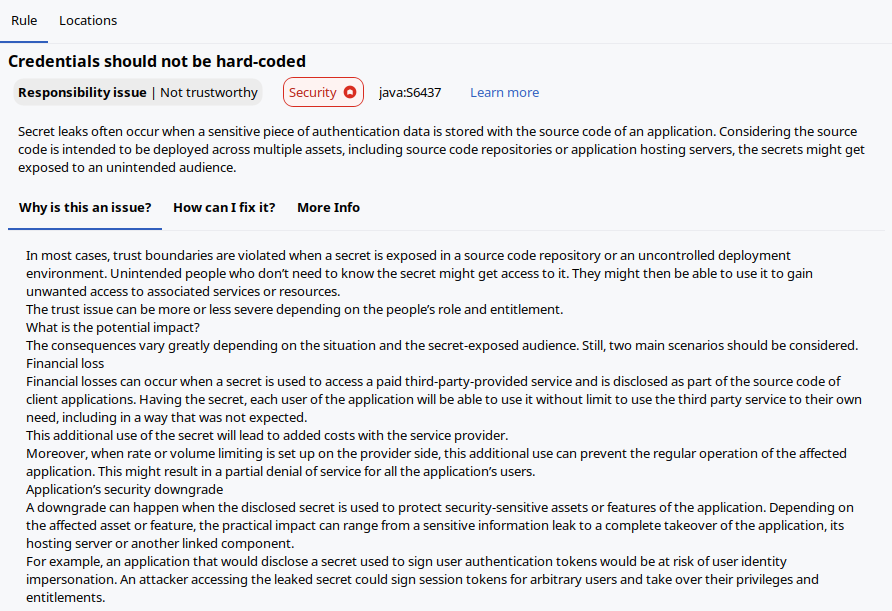
\includegraphics[width=3cm]{images/sonarlint-report.png}};
   \draw[gray,-Kite] ([xshift=6mm]dfg-constraints.south) to[out=-40,in=180] (sonar-com.west);
\end{uncoverenv}
\begin{onlyenv}<18-29|handout:2>
\onslide<18->{
   \pgfinterruptboundingbox
   \fill[white,fill opacity=.85] ([yshift=6mm]current page.south west) rectangle (current page.east|-persp.north);
   \endpgfinterruptboundingbox
   \node[draw=darkgray,fill=white,minimum width=4.2cm,minimum height=4.5cm,fill opacity=.93,rounded corners=3.45pt,thick,align=center,right] (@1) at ([xshift=-5mm,yshift=4mm]@code-file.west) {~\\[-5mm]{\onslide<19->{\usebox\ExampleCodeCfG}}};
   \node[above] at(@1.south) {\textbf{Code}};
}
\onslide<20->{
   \node[draw=darkgray,fill=white,minimum width=4cm,minimum height=4.5cm,fill opacity=.93,rounded corners=3.45pt,thick,right=7mm,align=center] (@2) at (@1.east) {%
   ~\\[-5mm]{\onslide<21->{\resizebox{4cm}!{\usebox\ExampleCFGofCode}}}%
   };
   \node[above] at(@2.south) {\textbf{Control Flow Graph}};
}
\onslide<23->{
   \node[draw=darkgray,fill=white,minimum width=4cm,minimum height=4.5cm,fill opacity=.93,rounded corners=3.45pt,thick,right=7mm,align=center] (@3) at (@2.east) {~\\[-5mm]{\onslide<24->{\resizebox{4cm}!{\usebox\ExampleLivenessofCode}}}};
   \pgfinterruptboundingbox
   \node[xshift=-12mm,yshift=4.2mm,draw=darkgray,fill=white,fill opacity=.93,rounded corners=3.45pt,thick,align=center,text width=4.5cm,scale=.65,font=\footnotesize,inner sep=1pt] at(@3.north east) {%
   \begin{align*}
      \mathbf{In}_n &= (\mathbf{Out}_n - \mathbf{Kill}_n) \cup \mathbf{Gen}_n \\
      \mathbf{Out}_n &= \begin{cases}
         \mathbf{BI} & n \text{~is End} \\
         \bigcup\limits_{m \in \text{succ}(n)} \mathbf{In}_m & \text{otherwise}
      \end{cases}
   \end{align*}
   With fixpoint iteration
   };
   \endpgfinterruptboundingbox
   \node[above] at(@3.south) {\textbf{Liveness}\textsuperscript{\smaller[2]\cite[p.\,26]{10.5555/1592955}}};
}
\end{onlyenv}
% by default iterated until reach fixpoint
\end{tikzpicture}
\end{lrbox}
\global\setbox\SonarLintShow=\copy\SonarLintShow
\begin{tikzpicture}[overlay,remember picture]
   \node[above=-1mm,xshift=.33mm] at(current page.south) {\usebox\SonarLintShow};
\end{tikzpicture}
\end{uncoverenv}
\begin{tikzpicture}[overlay,remember picture]
   \node[below left=4mm] at(current page.north east) {\Logo[2.5cm]{https://www.sonarsource.com/products/sonarlint/}{sonar}};
   \node[above right,yshift=4mm,bottom note] at(current page.south west) {\href{https://github.com/SonarSource}{github.com/SonarSource/sonar-java}};
   \only<23-|handout:2>{
      \node[above left,bottom note,yshift=4mm] at(current page.south east) {\cite{10.5555/1592955}~\citetitle{10.5555/1592955} (\citeauthor{10.5555/1592955})};
   }
\end{tikzpicture}
\end{frame}

\lstfs{11}
\begin{frame}[t,fragile]{\textcolor{gray}{SonarLint ---~}Unused Assignments}
\begin{itemize}
   \itemsep9pt
   \item<2-> Analyze \enquote{Dead Stores} {\onslide<3->{\smaller[2]\textcolor{gray}{(in 311\,loc\,/\,259\,cloc)}:}}
\begin{minted}[escapeinside=||]{java}
|\onslide<4->|int x = 0;
x = 42;|\onslide<1->|
\end{minted}
   \item<5-> Use \href{https://github.com/SonarSource/sonar-java/blob/50b7d48e5764545a78a7ef2bf84b8a5ff1f30b3e/java-frontend/src/main/java/org/sonar/java/cfg/LiveVariables.java\#L73}{liveness analysis} to obtain \(out_n\) of each basic block in the CFG
   \item<6-> Check if assignments (\bjava{x =}, \bjava{x++},~\ldots) are in \(out_n\) and resolved
   \item<7-> Check overwrites in the same basic block
   \item<8-> Minor special handling for \bjava{try-finally} blocks,~\ldots
\end{itemize}
\begin{tikzpicture}[overlay,remember picture]
   \node[below left=4mm] at(current page.north east) {\Logo[2.5cm]{https://www.sonarsource.com/products/sonarlint/}{sonar}};
   \node[above right,bottom note, yshift=4mm] at(current page.south west) {\href{https://github.com/SonarSource/sonar-java/blob/50b7d48e5764545a78a7ef2bf84b8a5ff1f30b3e/java-checks/src/main/java/org/sonar/java/checks/DeadStoreCheck.java\#L52}{Implementation of Rule S1854}};
   \begin{uncoverenv}<9-|handout:2>
      \xlstsetmintedstyle{plain number}
      \node[above left=2mm,yshift=5.5mm,text width=.75\paperwidth,fill=white,draw,rounded corners=3pt,inner ysep=0pt,fill opacity=.95,drop shadow={fill=lightgray!50}] at(current page.south east) {\lstfs{8}%
\begin{minted}[firstnumber=77,morekeywords={[3]{CFG,Block,LiveVariables}},xleftmargin=7mm,prebreak={}]{java}
LiveVariables liveVariables = LiveVariables.analyze(cfg);
// Liveness analysis provides information only for block boundaries, so we should do analysis between elements within blocks
for(CFG.Block block : cfg.blocks()) {
   checkElements(block, liveVariables.getOut(block), methodSymbol);
}
\end{minted}
      };
   \end{uncoverenv}
\end{tikzpicture}
\end{frame}


\begin{frame}[t,fragile]{\textcolor{gray}{SonarLint ---~}Hardcoded Credentials}
\begin{itemize}
   \itemsep8pt
   \item<2-> It does not always have to be that heavy! {\onslide<3->{\smaller[2]\textcolor{gray}{(116\,loc\,/\,87\,cloc may suffice)}}}
   \item<4-> For example, to identify hardcoded credentials:
{%
\lstfs{9}
\begin{minted}[escapeinside=||]{java}
|\onslide<5->|new PasswordAuthentication("password", "secret".toCharArray());|\onslide<1->|
\end{minted}
}\vspace*{-.85\baselineskip}
   \item<6-> Traverse the Abstract Syntax Tree~(AST)
   \item<7-> Check calls against a long \href{https://github.com/SonarSource/sonar-java/blob/3e2cb4478100a5ea082dde30004067579eef58a4/java-checks-aws/src/main/resources/org/sonar/java/checks/security/S6437-methods.json}{list of signatures} (currently 7664) with problematic indices
   \item<8-> Check if the arguments are \enquote{constant}\\
   \onslide<9->{\textcolor{gray}{visiting the dataflow links and checking for predefined \enquote{plain text}}}
\end{itemize}
\begin{tikzpicture}[overlay,remember picture]
   \node[below left=4mm] at(current page.north east) {\Logo[2.5cm]{https://www.sonarsource.com/products/sonarlint/}{sonar}};
   \node[above right,bottom note, yshift=4mm] at(current page.south west) {\href{https://github.com/SonarSource/sonar-java/blob/50b7d48e5764545a78a7ef2bf84b8a5ff1f30b3e/java-checks-aws/src/main/java/org/sonar/java/checks/security/HardCodedCredentialsShouldNotBeUsedCheck.java\#L43}{Implementation of Rule S6437}};
   % TODO: mark heuristics: list of signatures and constant check
   \begin{uncoverenv}<10-|handout:2>
      \xlstsetmintedstyle{plain number}
      \xlstblacklistlinenumbers{111}
      \node[above left=2mm,yshift=5.5mm,text width=.85\paperwidth,fill=white,draw,rounded corners=3pt,inner ysep=0pt,fill opacity=.95,drop shadow={fill=lightgray!50}] at(current page.south east) {\lstfs{8}%
\begin{minted}[firstnumber=107,morekeywords={[3]{ExpressionTree,JavaFileScannerContext,Location,ISSUE_MESSAGE}},xleftmargin=7mm,prebreak={}]{java}
for (int targetArgumentIndex : method.indices) {
   ExpressionTree argument = arguments.get(targetArgumentIndex);
   var secondaryLocations = new ArrayList<JavaFileScannerContext.Location>();
   if (isExpressionDerivedFromPlainText(argument, 
               secondaryLocations, new HashSet<>())) {
      reportIssue(argument, ISSUE_MESSAGE, secondaryLocations, null);
   }
}
\end{minted}
      };
   \end{uncoverenv}
\end{tikzpicture}
\end{frame}

\newsavebox\pinguLook
\savebox\pinguLook{\scalebox{.65}{\tikz{\pingu[left eye wink,right wing wave,magnifier right,small,tie,deer hat]}}} 

\subsubsection{LiSA}
\againframe<7,18|handout:4>{tool-slide}
\begin{frame}{LiSA}
\begin{itemize}
   \itemsep6.5pt
   \item<2-> \textcolor{gray}{(Largely)} Language Independent \underline{Li}brary for \underline{S}tatic \tikzmarknode{lisa-alts}{\underline{A}nalysis}
   \item<4-> Custom frontends for Rust, Go, Python, EVM,~\ldots
\end{itemize}
\begin{tikzpicture}[overlay,remember picture]
   \node[below left=4mm] at(current page.north east) {\Logo[2cm]{https://github.com/lisa-analyzer/lisa}{lisa}};
   \node[above right,yshift=4mm,bottom note] at(current page.south west) {\href{https://github.com/lisa-analyzer/lisa}{github.com/lisa-analyzer/lisa}};
   \onslide<3->{%
      \draw[-Kite,gray] ([xshift=1.5mm]lisa-alts.east) to[out=0,in=180] ++(6mm,2mm) node[right,bottom note,align=left] {Similar to \href{https://mopsa.lip6.fr/}{Mopsa} or \href{https://github.com/antoinemine/apron}{Apron}};
   }
\end{tikzpicture}
\begin{uncoverenv}<5->
\begin{tikzpicture}[o/.style={outer sep=0pt,inner sep=0pt},remember picture]
   \node[o] (@) at (0,0) {\usebox\CodeFile};
   \node[above=2.5mm,xshift=1.15mm,gray] at(@.north) {\textbf{\normalsize Input}};
\pgfonlayer{background}
\scope[transparency group,opacity=.4]
\node[o,rotate around={-30:(@.south east)},anchor=south east] at(@.south east) {\usebox\CodeFile};
\node[o,rotate around={-12:(@.south east)},anchor=south east] at(@.south east) {\usebox\CodeFile};
\endscope
\endpgfonlayer
\coordinate (@) at(@.east);
\foreach[count=\i] \usecase/\targeti in {{\raisebox{1pt}{Textual}}/1,Syntactical/0, Semantical/0, Historical/1, Annotated/0, {\raisebox{-3pt}{Metadata,~\ldots}}/1} { % program spectra, hardware, contexts, ...
\pgfmathsetmacro\rot{-24*\i+66}
      \path ([xshift=.5mm]@.east)++(\rot+10:1mm) coordinate (@a);
      \fill[opacity=.18,gray] (@a.east) -- ++(\rot:1.5cm) arc (\rot:\rot+20:1.5cm) -- cycle;
      \draw[thick,gray] (@a.east)++(\rot:1.5cm) arc (\rot:\rot+20:1.5cm);
      \tikzset{@/.style={}}
      \ifnum\targeti=1relax
         \only<7->{
            \tikzset{@/.style={opacity=.2}}
         }
      \fi
      \path (@a.east) -- ++(1.05*\rot+10:1.6cm) node[right,font=\small,darkgray,@] (@uc-\i) {\vphantom{a}\smash{\usecase}};
}
\coordinate (@east) at (current bounding box.east);
\onslide<8->{%
   \draw[decoration={brace},decorate,gray] ([yshift=.5mm]@uc-2.north east-|@uc-3.north east) -- ([yshift=-.5mm]@uc-3.south east) node[midway,right=1mm,font=\footnotesize,align=left] (jbc) {Construct CFG}; % using java byte code is rather common
}
\node[above=1.65mm,xshift=1mm,gray] at(current bounding box.north) {\textbf{\normalsize Perspectives}};
\begin{onlyenv}<-5|handout:0>
\node[right,yshift=-7mm,xshift=1cm,align=left,font=\small,darkgray,text width=3.25cm] (@techn) at(@east){{{{Text/Code Search}\strut}}~\\[4mm]\strut{{{Clustering}}}~\\[4mm]\strut{{{Abstract Domains}}}~\\[4mm]\strut{{{Dataflow Constraints}}}~\\[1mm]\strut{{\centerline{\footnotesize\(\vdots\)}}}};
\node[above=1.5mm,gray,xshift=-4.5mm] at(@techn.north) {\textbf{\normalsize Theory}};
\scope[gray,line cap=round]
   \draw ([yshift=1.5pt]@uc-1.east) -- ([yshift=-2.5mm]@techn.north west);
   \draw ([yshift=1.5pt]@uc-2.east) -- ([yshift=-2.5mm]@techn.north west);
   \draw[densely dotted] ([yshift=1.5pt]@uc-3.east) -- ([yshift=-2.5mm]@techn.north west);
   \draw ([yshift=1.5pt]@uc-1.east) -- ([yshift=-10.5mm]@techn.north west);
   \draw ([yshift=0pt]@uc-2.east) -- ([yshift=-10.5mm]@techn.north west);
   \draw ([yshift=1.5pt]@uc-4.east) -- ([yshift=-10.5mm]@techn.north west);
   
   \draw ([yshift=-1pt]@uc-2.east) -- ([yshift=-18.5mm]@techn.north west);
   \draw ([yshift=-1pt]@uc-3.east) -- ([yshift=-18.5mm]@techn.north west);
   \draw ([yshift=1.5pt]@uc-5.east) -- ([yshift=-18.5mm]@techn.north west);
   
   \draw ([yshift=-1pt]@uc-2.east) -- ([yshift=-26mm]@techn.north west);
   \draw ([yshift=-1pt]@uc-3.east) -- ([yshift=-26mm]@techn.north west);
\endscope
   
   \node[right=7.5mm] (@) at(current bounding box.east) {\resizebox*!{2.85cm}{\usebox\UiBox}};
   \scope[transparency group,opacity=.5,every path/.append style={line cap=round,line width=.5pt}]
      \draw[-Kite,gray] ([yshift=-2.5mm,xshift=-6.5mm]@techn.north east) to[out=0,in=180] ([xshift=1.5mm,yshift=-6.35mm]@.west);
      \draw[-Kite,gray] ([yshift=-10.5mm,xshift=-18.5mm]@techn.north east) to[out=0,in=180] ([xshift=7.15mm,yshift=-1.35mm]@.west);
      \draw[-Kite,gray] ([yshift=-18.5mm,xshift=-6.25mm]@techn.north east) to[out=0,in=180] ([xshift=26.15mm,yshift=-9.35mm]@.west);
      \draw[-Kite,gray] ([yshift=-26mm,xshift=-2.5mm]@techn.north east) to[out=0,in=180] ([xshift=26.15mm,yshift=-9.35mm]@.west);
   \endscope
   \node[above, gray] at(@.north) {\tiny \textbf{\normalsize Communicate} or \textbf{\normalsize Use}};
\end{onlyenv}
\onslide<9->{%
   \draw[gray,-Kite] (@uc-5.east) to[out=0,in=180] ++(6.5mm,2mm) node[below right,font=\footnotesize,yshift=.7\baselineskip,align=left] {(Depends on Frontend)};
}
\onslide<10->{%
   \draw[gray,Kite-] (jbc) to[out=80,in=260] ++(2mm,7.5mm) node[above,bottom note,align=center] {Language-Specific\\Frontends};
}
\onslide<11->{%
   \draw[gray,-Kite] ([xshift=-4.25mm]jbc.south) to[out=-80,in=180] ++(6mm,-3mm) node[right,bottom note,align=center] (cfg-dr-note) {\href{https://github.com/lisa-analyzer/lisa/blob/2543b47cfdb0a968a064d16f000fa0ad1d823125/lisa/lisa-analyses/src/main/java/it/unive/lisa/analysis/dataflow/Liveness.java\#L25}{Liveness}, \href{https://github.com/lisa-analyzer/lisa/blob/cd351110a5c47f69a16f0ca025058ad5a53976cb/lisa/lisa-analyses/src/main/java/it/unive/lisa/analysis/numeric/Pentagon.java\#L47}{Pentagons},~\ldots};
}
\onslide<12->{
   \node[above=3.5mm,gray,xshift=20.5mm] (theory) at(@techn.north) {\textbf{\normalsize Theory}};
}
\onslide<13->{
   \node[below=1mm,align=right] (a-domains) at(theory.south) {\small Abstract Domains}; % many parameterized
}
\onslide<14->{
   \draw[gray,Kite-Kite] (a-domains.south) to[bend left] (cfg-dr-note.east);
}
\begin{uncoverenv}<15->
   \node[right=20.5mm,yshift=-.5mm,gray] (communicate) at(theory.east) {\textbf{\normalsize Use}};
   \node[below=1mm,thick,inner sep=0pt,align=center,font=\small] (lisa-use) at(communicate.south) {Extension Interfaces\\Fixpoint Iterations,\\\ldots};
   \draw[gray,-Kite] ([xshift=1mm]a-domains.south) to[out=-40,in=180] (lisa-use.west);
\end{uncoverenv}
\onslide<16->{%
   \node[above left=2mm,yshift=3mm] (@ping) at(current page.south east) {\usebox\pinguLook};
   \node[left,gray,align=right] at(@ping.west) {Let's have a\\closer look!};
}
\end{tikzpicture}
\end{uncoverenv}
\end{frame}

\begin{lrbox}{\IntervalLattice}
\scriptsize
\begin{tikzpicture}[line cap=round,x=6.5mm,y=6.5mm,gray]
   \matrix (A) [matrix of nodes, row sep=2.5mm, column sep=-2mm]
   {
       & &  & \I{-1}{\infty} & & & \\
       & & \I{-1}{1} & \ldots & \I{0}{2} & & \\
      & \I{-1}{0} & \ldots & \I01 & \ldots & \I{1}{2} & \\
      \I{-1}{-1} & \ldots & \I00 & \ldots & \I11 & \ldots & \I22 \\
      & & & \absexpr{\bot} & & & \\
   };
   \scope[line cap=round]
   \draw (A-2-3) -- (A-3-2) -- (A-4-1) -- (A-5-4);
   \draw (A-3-6) -- (A-4-7) -- (A-5-4);
   \draw (A-3-2) -- (A-4-3) -- (A-3-4) (A-3-4) -- (A-4-5) -- (A-3-6);
   \draw (A-2-3) -- (A-3-4) (A-3-4) -- (A-2-5) -- (A-3-6);
   \draw (A-4-3) -- (A-5-4) -- (A-4-5);
   \draw[densely dotted] (A-2-5) -- (A-1-4) -- (A-2-3);
   \draw[densely dotted] (A-5-4) -- ++(-1,0.05)  (A-5-4) -- ++(1,0.05);
   \foreach[count=\y] \i in {4,3,2,1} {
      \draw[densely dotted] (A-\y-\i.north west) -- ++(-.4,0.14);
      \node[left=3.5mm] at(A-\y-\i.west) {\footnotesize\ldots};
      \pgfmathsetmacro\other{int(8-\i)}
      \draw[densely dotted] (A-\y-\other.north east) -- ++(.4,0.14);
      \node[right=3.5mm] at(A-\y-\other.east) {\footnotesize\ldots};
   }
   \node[above=3.5mm] (pz) at(A-1-4.north) {\absexpr{\top}};
   \draw[densely dotted] (pz) -- ++(-1.25,-0.1) (pz) -- ++(1.25,-0.1);
   \endscope
\end{tikzpicture}
\end{lrbox}

\makeatletter
% https://github.com/lisa-analyzer/lisa/blob/bd00779ab87e1cd31ed01b97d9b0e71b922f5bcf/lisa/lisa-analyses/src/main/java/it/unive/lisa/analysis/numeric/Interval.java#L47
\def\FakeLineNumber#1{\llap{\xlstGetStyle{linenumbers}\href{https://github.com/lisa-analyzer/lisa/blob/bd00779ab87e1cd31ed01b97d9b0e71b922f5bcf/lisa/lisa-analyses/src/main/java/it/unive/lisa/analysis/numeric/Interval.java\#L#1}{\underline{\xlst@lst@num@consume{#1}}}~~~}}

\begin{frame}[fragile]{\textcolor{gray}{LiSA ---~}Interval Analysis\textsuperscript{\color{gray}\smaller[2]\cite[p.\,389]{cousout2021principles}}}
\lstfs{8}
\begin{uncoverenv}<7->
{\scriptsize\color{gray}\href{https://github.com/lisa-analyzer/lisa/blob/bd00779ab87e1cd31ed01b97d9b0e71b922f5bcf/lisa/lisa-analyses/src/main/java/it/unive/lisa/analysis/numeric/Interval.java}{\hbox{\faFileCodeO~}lisa-analyses/src/main/java/it/unive/lisa/analysis/numeric/Interval.java} (simplified)}
\AnimateCode{onslide={o1:{2},-,o3:{4,...,7},o8:{9,...,13},-,0,-},first slide=7,handout=12/1}
\begin{minted}[morekeywords={Interval,IntInterval,Constant,ProgramPoint,SemanticOracle,SemanticException},escapeinside=||]{java}
|\FakeLineNumber{57}|Interval TOP = new Interval(IntInterval.INFINITY);
|\onslide<8->{\FakeLineNumber{62}}\onslide<8->|Interval BOTTOM = new Interval(null);|\medskip|
|\onslide<9->{\FakeLineNumber{273}}\onslide<9->|public Interval lubAux(Interval other) {
|\onslide<9->{\FakeLineNumber{276}}\onslide<9->|   var newL = getLow().min(other.getLow());
|\onslide<9->{\FakeLineNumber{277}}\onslide<9->|   var newH = getHigh().max(other.getHigh());
|\onslide<9->{\FakeLineNumber{278}}\onslide<9->|   return new Interval(newLow, newHigh);
|\onslide<9->{\FakeLineNumber{279}}\onslide<9->|}|\medskip\onslide<1->|
|\onslide<10->{\FakeLineNumber{282}}\onslide<10->|public Interval glbAux(Interval other) {
|\onslide<10->{\FakeLineNumber{284}}\onslide<10->|   var newL = getLow().max(other.getLow());
|\onslide<10->{\FakeLineNumber{285}}\onslide<10->|   var newH = getHigh().min(other.getHigh());|\onslide<1->|
|\onslide<10->{\FakeLineNumber{287}}\onslide<11->|   if(newLow.compareTo(newHigh) > 0) return bottom();
|\onslide<11->{\FakeLineNumber{289}}\onslide<10->|   return new Interval(newLow, newHigh);
|\onslide<10->{\FakeLineNumber{290}}\onslide<10->|}|\vspace*{-5mm}\onslide<1->|
\end{minted}
\endAnimateCode
\onslide<12->{\footnotesize\textit{Widening, Narrowing, Assume, Satisfies,~\ldots}}
\end{uncoverenv}
\begin{tikzpicture}[overlay,remember picture]
   \node[above right,yshift=4mm,bottom note] at(current page.south west) {\cite{cousout2021principles}~\citetitle{cousout2021principles} (\citeauthor{cousout2021principles})};
   \onslide<2->{\node[above left,yshift=5mm,scale=.8] (int-latt) at(current page.south east) {\usebox\IntervalLattice};}
   \onslide<3->{%
      \node[above,text width=5cm,font=\scriptsize] at(int-latt.north) {%
         \begin{align*}
            \top &= \I{-\infty}{\infty} \tag*{Top}\\
            \onslide<4->{\bot} &\onslide<4->{{}= \absexpr{\emptyset} \only<4->{\tag*{Bottom}}} \\
            \onslide<5->{\absexpr{\Lub_{k}} \I{\ell_k}{h_k}} &\onslide<5->{{}=\I{\min(\ell_k)}{\max(h_k)} \only<5->{\tag*{Join}}} \\
            \onslide<6->{\absexpr{\Glb_{k}} \I{\ell_k}{h_k}} &\onslide<6->{{}=\I{\max(\ell_k)}{\min(h_k)} \only<6->{\tag*{Meet}}}
            % hidden for now
            % \I{\ell_l}{h_l} \absexpr{\widen} \I{\ell_r}{h_r} &= \I{\ell_l > \ell_r ? -\infty : \ell_l}{h_l < h_r ? \infty : h_l} \tag*{Widening}
         \end{align*}
      };
   }
\end{tikzpicture}
\end{frame}

\begin{frame}[fragile]{\textcolor{gray}{LiSA ---~}Interval Analysis\textsuperscript{\color{gray}\smaller[2]\cite[p.\,389]{cousout2021principles}}\hfill Semantics}
\lstfs{8}
\onslide<2->{When to create which interval?}\\*
\begin{uncoverenv}<3->
{\scriptsize\color{gray}\href{https://github.com/lisa-analyzer/lisa/blob/bd00779ab87e1cd31ed01b97d9b0e71b922f5bcf/lisa/lisa-analyses/src/main/java/it/unive/lisa/analysis/numeric/Interval.java}{\hbox{\faFileCodeO~}lisa-analyses/src/main/java/it/unive/lisa/analysis/numeric/Interval.java} (simplified)}
\AnimateCode{onslide={o1:{3,...,8},-,-,o9:{10},o11:{12},o1:{3,...,12},-},first slide=3,handout=8/1}
\preto\ldots{\color{lightgray}}% hijack the literate
\begin{minted}[morekeywords={Interval,IntInterval,Constant,ProgramPoint,SemanticOracle,SemanticException},escapeinside=||]{java}
|\onslide<3->{\FakeLineNumber{144}}\onslide<3->|public Interval evalNonNullConstant(Constant constant,
|\onslide<3->{\FakeLineNumber{146}}\onslide<3->|      ProgramPoint pp, SemanticOracle oracle) {
|\onslide<4->{\FakeLineNumber{148}}\onslide<4->|   if(constant.getValue() instanceof Integer) {
|\onslide<4->{\FakeLineNumber{149}}\onslide<4->|      var i = (Integer) constant.getValue();
|\onslide<4->{\FakeLineNumber{150}}\onslide<4->|      return new Interval(i, i);
|\onslide<4->{\FakeLineNumber{151}}\onslide<4->|   }
|\onslide<5->{\FakeLineNumber{152}}\onslide<5->|   return top();|\onslide<1->|
|\onslide<3->{\FakeLineNumber{153}}\onslide<3->|}|\medskip\onslide<1->|
|\onslide<6->{\FakeLineNumber{157}}\onslide<6->|public Interval evalUnaryExpression(UnaryOperator op,
|\onslide<6->{\FakeLineNumber{158}}|    Interval arg, :ldots:) { :ldots: }|\onslide<1->|
|\onslide<7->{\FakeLineNumber{188}}\onslide<7->|public Interval evalBinaryExpression(BinaryOperator op,
|\onslide<7->{\FakeLineNumber{189}}|    Interval left, |\tikzmarknode{fold-like-marker}{\strut}|Interval right, :ldots:) { :ldots: }|\onslide<1->|
\end{minted}
\endAnimateCode
\end{uncoverenv}
\begin{tikzpicture}[overlay,remember picture]
   \node[above right,yshift=4mm,bottom note] at(current page.south west) {\cite{cousout2021principles}~\citetitle{cousout2021principles} (\citeauthor{cousout2021principles})};
   \node[above left,yshift=5mm,scale=.8] (int-latt) at(current page.south east) {\usebox\IntervalLattice};
   \onslide<9->{%
      \coordinate (@) at(fold-like-marker);
      \draw[Kite-,gray] ([xshift=5mm,yshift=-1mm]@) to[out=280,in=180] ++(3mm,-4mm) node[right,bottom note] {Fold-like Evaluation};
   }
\end{tikzpicture}
\end{frame}

\subsubsection{flowR}
\let\T\texttt
\def\Content#1#2{#1\\[-.6ex]\smaller\textit{\color{gray}#2}}
\againframe<7,21|handout:7>{tool-slide}
\newsavebox\ShookPingu
\savebox\ShookPingu{\tikz{\pingu[wings shock,eyes shock,tie]}}

\newsavebox\PartyPingu

\savebox\PartyPingu{\tikz{\pingu[wings wave,eyes wink,tie=purple]}}
\begin{frame}[fragile]{flowR}
   \lstfs{8}
   \begin{itemize}
      \itemsep6pt
      \item<2-> A static analysis framework for R
      \item<3-> Developed here, at Ulm University \onslide<4->{\smash{\raisebox{-4pt}{\resizebox*!{1.5\baselineskip}{\usebox\PartyPingu}}}}\\*[1mm]
         \onslide<5->{\color{gray}{\only<6->{\bfseries\color{black}}Florian Sihler}, \color{gray}Julian Schubert, Lars Pfrenger, Johanna Scheck, Lukas Pietzschmann,\\Ruben Dunkel, Felix Schlegel, Pascal Deusch,~\ldots}%
      \item<7-> Let's get back to R:
\begin{uncoverenv}<8->
   \begin{columns}[onlytextwidth,c]
\column{.04\linewidth}
\column{.3\linewidth}
\begin{minted}{R}
x <- 4
f <- function() x
body(f) <- quote(y)
y <- 42
f() # 42
\end{minted}
\column{.365\linewidth}
\color{black}\vspace*{-\baselineskip}%
\begin{minted}{R}
`if` <- function(...) 42
if(TRUE) print(3) # 42
\end{minted}
\column{.3\linewidth}
\color{black}\vspace*{-\baselineskip}%
\begin{minted}{R}
x <- 2
`<-` <- `*`
x <- 21 # 42
\end{minted}
\end{columns}
\end{uncoverenv}
\item<9-> We have to intertwine dataflow- and control-flow analysis\ldots
\end{itemize}
   \begin{tikzpicture}[overlay,remember picture]
      \node[below left=4mm,yshift=2mm] at(current page.north east) {\Logo[2.1cm]{https://github.com/flowr-analysis/flowr}{flowr}};
      \node[above right,yshift=4mm,bottom note] at(current page.south west) {\href{https://github.com/flowr-analysis/flowr}{github.com/flowr-analysis/flowr}};
   \end{tikzpicture}
\end{frame}

\def\SwitchTo#1#2{#1}
\def\GrayBack{\fill[white,opacity=.7] (current bounding box.south west) rectangle (current bounding box.north east);}
\def\XShift{3.5mm}%
\newsavebox\CodeBoxA
% \begin{frame}[fragile,c]{\textcolor{gray}{flowR ---} Architecture}
% \centering
% \begin{tikzpicture}[All Soft, br/.style={fill=white,draw=black,drop shadow={fill=lightgray!50},minimum width=2.5cm,minimum height=1.5cm,signal,signal from=west,signal to=east,signal pointer angle=125,rounded corners=2pt},k/.style={below,font=\footnotesize,xshift=-.33mm,color=darkgray},m/.style={above,font=\scriptsize,xshift=-.33mm,color=gray},BaseGray,Link/.style={
%    draw=SoftGray,
%    line width=1.5pt,
%    line cap=round,
%    line join=round,
%    -%
% }]
%    \tikzset{a/.style={opacity=.5}}
%    \coordinate (@) at (0,0);

%    \onslide<2->{
%       \node[br,right=\XShift] (@) at (@.east) {};
%       \coordinate (@parse) at (@.north west);
%       \coordinate (@parse-l) at (@.south west);
%       \node (r-conv) at (@) {\SwitchTo{\usebox\Parsing}{\,Parse}};
%       \pgfinterruptboundingbox\node[k] at (@.south) {\SwitchTo{Parse}{}};\endpgfinterruptboundingbox
%    }
%       % \onslide<4->{\node[m] at (@.north) {\texttt{parse}\,\(\to\)\,XML};}

%    \onslide<3->{
%       \node[br,right=\XShift] (@) at (@.east) {};
%       \node[align=center] (first-ast) at (@) {\SwitchTo{\usebox\FirstAst}{Normalize}};
%       \coordinate (@normalize) at (@.north west);
%       \pgfinterruptboundingbox\node[k,align=center] at (@.south) {\SwitchTo{Normalize}{}};\endpgfinterruptboundingbox
%       % \onslide<6->{\node[m] at (@.north) {in TypeScript};}
%       \coordinate (@l) at(@.south west);
%    }
%    \scope
%    \onslide<4->{
%       \node[br,right=\XShift] (@) at (@.east) {};
%       \coordinate (@dataflow) at (@.north east);
%       \coordinate (@dataflow-l) at (@.south east);
%       \node (dataflow) at (@) {\SwitchTo{\usebox\DataFlow}{\;Dataflow}};
%       \pgfinterruptboundingbox\node[k] at (@.south) {\SwitchTo{Dataflow}{}};\endpgfinterruptboundingbox
%    }
%    \endscope
%    \scope
%    \onslide<5->{
%       \node[br,right=\XShift] (@) at (@.east) {};
%       \pgfinterruptboundingbox\node (slicing) at (@) {\SwitchTo{\usebox\Slicing}{\,Slice}};\endpgfinterruptboundingbox
%       \node[k] at (@.south) {\SwitchTo{Slice}{}};
%       \coordinate (@slice) at (@.north west);
%       \coordinate (@slice-l) at (@.south west);
%       % \onslide<9->{\node[m] at (@.north) {Weiser~\cite{weiser_program_1984}};}
%    }
%    \endscope
%    \onslide<6->{
%       \node[br,right=\XShift] (@) at (@.east) {};
%       \node (reconstruct) at (@) {\SwitchTo{\usebox\Reconstruct}{\; Reconstruct}};
%       \pgfinterruptboundingbox\node[k] at (@.south) {\SwitchTo{Reconstruct}{}};\endpgfinterruptboundingbox
%       \coordinate (@r) at(@.south east);
%       \coordinate (@reconstruct) at (@.north east);
%       \coordinate (@reconstruct-l) at (@.south east);
%    }
% \end{tikzpicture}\medskip
% \begin{onlyenv}<7->
% \lstfs{7}
% \hspace*{1.5cm}%
% \begin{lrbox}\CodeBoxA
% \begin{minted}[deletekeywords={sum,prod},escapeinside={/*}{*/}]{R}
% sum  <- 0
% prod <- 1
% n    <- 10

% for (i in 1:(n-1)) {
%    sum  <- sum + i
%    prod <- prod * i
% }

% cat("Sum:"/*\color{black}*/, /*\texttt{\only<8->{\textbf}{sum}}*//*\color{black}*/, "\n")
% cat/*\color{black}*/("Product:"/*\color{black}*/, prod, "\n"/*\color{black}*/)
% \end{minted}
% \end{lrbox}
% \begin{tikzpicture}
% \begin{uncoverenv}<7->
% \node (@) at (0,0) {%
%    \usebox\CodeBoxA
% };
% \end{uncoverenv}

% \begin{uncoverenv}<9->
%    \node[right=2.5cm] (@2) at (@.east) {%
% \AnimateCode{onslide={o8:{7,5,4,3,1}}, first slide=9,handout={9/1}}
% \begin{minted}[deletekeywords={sum,prod},escapeinside={/*}{*/}]{R}
% sum  <- 0
% prod <- 1
% n    <- 10

% for (i in 1:(n-1)) {
%    sum  <- sum + i
%    prod <- prod * i
% }

% cat("Sum:", sum, "\n")
% cat("Product:", prod, "\n")
% \end{minted}
% \endAnimateCode
%    };
% \end{uncoverenv}
% \onslide<8->{
%    \draw[-Kite,line cap=round] ([xshift=5mm]@.east) to[edge node={node[above] {\footnotesize\texttt{slice({\xlstGet{linenumbers}{\footnotesize10}}\footnotesize\color{black}, \textbf{sum})}}}] ([xshift=-5mm]@2.west);
% }
% \end{tikzpicture}\hspace*{-2cm}
% \end{onlyenv}
% \begin{tikzpicture}[overlay,remember picture]
%    \node[below left=4mm,yshift=2mm] at(current page.north east) {\Logo[2.1cm]{https://github.com/flowr-analysis/flowr}{flowr}};
%    \node[above right,yshift=4mm,bottom note] at(current page.south west) {\href{https://github.com/flowr-analysis/flowr/tree/main/src/dataflow}{github.com/flowr-analysis/flowr/tree/main/src/dataflow}};
% \end{tikzpicture}
% \end{frame}






\lstfs{8}
\tikzset{K/.style={midway,#1=-.5mm,font=\smaller[3]}}
\newsavebox\FinalDataFlow
\colorlet{lgray}{gray!50!white}
\def\MarkBox#1{#1}%TODO: \fcolorbox{lgray}{white}{#1}}
\newcommand\MarkAt[3][0]{\setbox0=\hbox{~#3~}\makebox[\wd0+1mm][c]{\null\hfill\only<#2|handout:#1>{\bfseries\fboxsep=1pt\expandafter\larger\MarkBox}{\smash{#3}}\null\hfill}}
\newsavebox\EmptyEnvBox
\tikzset{%
   Env/.style={text width=1.85cm,rounded corners=2pt,fill=white,font=\footnotesize},
}%
\def\GetWith#1{\tikz{%
\node[Env] (@) {\strut#1};
\pgfonlayer{background}
\fill[rounded corners=2pt,fill=lgray] ([shift={(.4mm,.4mm)}]@.north east) rectangle ([shift={(-.4mm,-.4mm)}]@.south west);
\pgfinterruptboundingbox
\node[above right,gray] at([xshift=-1mm]@.north west) {\scriptsize Environment};
\endpgfinterruptboundingbox
\endpgfonlayer
}}
\newsavebox\EnvBox
\setbox\EnvBox=\hbox{}
\savebox\EmptyEnvBox{\GetWith{}}
\def\mto#1{\kern1.5pt$\mapsto$\kern1.5pt\bIndexR{#1}}
\newsavebox\BoxWithX \savebox\BoxWithX{\GetWith{x\mto{x_0}}}
\newsavebox\BoxWithXY \savebox\BoxWithXY{\GetWith{x\mto{x_0},\,y\mto{y_0}}}
\newsavebox\BoxWithZ \savebox\BoxWithZ{\GetWith{z\mto{z_0}}}
\newsavebox\BoxWithFull \savebox\BoxWithFull{\GetWith{x\mto{x_0},\,y\mto{y_0},\,\allowbreak z\mto{z_0}}}
\newcommand<>\OpaOn[1]{\tikzset{@@/.style={}}\only#2{\tikzset{@@/.style={opacity=.4}}}\scope[transparency group,@@]#1\endscope}

\tikzset{
   comm/.style={rectangle,draw=gray,text width=9mm,align=center,minimum height=5mm,font=\ttfamily,fill=white,fill opacity=1,drop shadow={fill=lightgray!50}},
   d/.style={comm,rounded corners=2pt},
   u/.style={comm,rounded rectangle},
   T/.style={font=\scriptsize,gray}
}
\def\WithGraph#1{\tikz{%
#1
\pgfinterruptboundingbox
\node[above=-1.25mm,gray] at(@.north) {\scriptsize\strut Graph};
\endpgfinterruptboundingbox
}}

\iffalse

\newsavebox\XUseGraph \savebox\XUseGraph{\WithGraph{\node[u] (@) at (0,0) {x\textsubscript{0}};}}
\newsavebox\XDefGraph \savebox\XDefGraph{\WithGraph{\node[d] (@) at (0,0) {x\textsubscript{0}};}}
\newsavebox\YUseGraph \savebox\YUseGraph{\WithGraph{\node[u] (@) at (0,0) {y\textsubscript{0}};}}
\newsavebox\ZUseGraph \savebox\ZUseGraph{\WithGraph{\node[u] (@) at (0,0) {z\textsubscript{0}};}}
\newsavebox\YDefGraph \savebox\YDefGraph{\WithGraph{\node[d] (@) at (0,0) {y\textsubscript{0}};}}
\newsavebox\XBUseGraph \savebox\XBUseGraph{\WithGraph{\node[u] (@) at (0,0) {x\textsubscript{1}};}}
\newsavebox\YBUseGraph \savebox\YBUseGraph{\WithGraph{\node[u] (@) at (0,0) {y\textsubscript{1}};}}
\newsavebox\XYBUseGraph \savebox\XYBUseGraph{\WithGraph{\node[u] (@) at (0,0) {y\textsubscript{1}}; \node[u,below=2mm] at (@.south) {x\textsubscript{1}};}}
\newsavebox\XYYBUseGraph \savebox\XYYBUseGraph{\WithGraph{%
   \node[u] (y) at (0,0) {y\textsubscript{1}};
   \node[u,below=2mm] (x) at (y.south) {x\textsubscript{1}};
   \node[d,left=4mm] (z) at (current bounding box.west) {z\textsubscript{0}};
   \draw[-Kite] (z) -- (x);
   \draw[-Kite] (z) -- (y);
   \coordinate(@) at(current bounding box.north);
}}
\newsavebox\FullUseGraph \savebox\FullUseGraph{\WithGraph{%
   \node[u] (y) at (0,0) {y\textsubscript{1}};
   \node[u,below=2mm] (x) at (y.south) {x\textsubscript{1}};
   \node[d,left=4mm] (z) at (current bounding box.west) {z\textsubscript{0}};
   \node[d,right=4mm] (xb) at(x.east) {x\textsubscript{0}};
   \node[d,right=4mm] (yb) at(y.east) {y\textsubscript{0}};
   \draw[-Kite] (z) -- (x);
   \draw[-Kite] (z) -- (y);
   \draw[densely dotted,-Kite] (x) -- (xb);
   \draw[densely dotted,-Kite] (y) -- (yb);
   \coordinate(@) at(current bounding box.north);
}}

\begin{frame}[fragile]{\textcolor{gray}{flowr ---} Dataflow}
% TODO: complete from 2.17 with read-graphs propagation
\hypertarget<1>{@DataFlow}{}%
\lstfs{8}
\begin{minted}[escapeinside={/*}{*/},lineskip=4pt]{IndexR}
/*\onslide<2->*/x_0 <- 21
y_0 <- 2
z_0 <- x_1 * y_1/*\onslide<1->*/
\end{minted}
\begin{center}
\begin{onlyenv}<3|handout:0>
\begin{forest}
   T, for tree={l sep=2mm,s sep=5mm,font=\footnotesize}
   [exprlist, s sep=2cm, l sep=0mm
      [\Content{assignment}{\LeftArrow}, edge label={node[K=above,sloped] {1}}
         [\Content{symbol}{x}, edge label={node[K=above,sloped] {target}}]
         [\Content{number}{21}, edge label={node[K=above,sloped] {source}}]
      ]
      [\Content{assignment}{\LeftArrow}, edge label={node[K=right] {2}},before computing xy={s/.average={s}{siblings}},
         [\Content{symbol}{y}, edge label={node[K=above,sloped] {target}}]
         [\Content{number}{2}, edge label={node[K=above,sloped] {source}}]
      ]
      [\Content{assignment}{\LeftArrow}, edge label={node[K=above,sloped] {3}}
         [\Content{symbol}{z}, edge label={node[K=above,sloped] {target}}]
         [\Content{binary-op}{\raisebox{-5pt}{\large*}}\vspace*{-3mm}, edge label={node[K=above,sloped] {source}},
            [\Content{symbol}{x}, edge label={node[K=above,sloped] {lhs}}]
            [\Content{symbol}{y}, edge label={node[K=above,sloped] {rhs}}]
         ]
      ]
   ]
\end{forest}
\end{onlyenv}
\begin{onlyenv}<4-|handout:1>
\begin{lrbox}\FinalDataFlow
\begin{forest}
   T, for tree={l sep=2mm,s sep=1.5cm, s sep-=5mm,font=\footnotesize}
   [\MarkAt{5,6,21}{exprlist}, s sep=2cm, l sep=0mm,name=exprlist
      [\MarkAt{7,11}{\LeftArrow}, edge label={node[K=above,sloped] {1}},name=la1
         [\MarkAt{8,9}{x\RCodeIndex0}, edge label={node[K=above,sloped] {target}},name=x1]
         [\MarkAt{10}{21}, edge label={node[K=above,sloped] {source}},name=21]
      ]
      [\MarkAt{12,13}{\LeftArrow}, edge label={node[K=right] {2}},name=la2,before computing xy={s/.average={s}{siblings}}
         [y\RCodeIndex0, edge label={node[K=above,sloped] {target}},name=y1]
         [2, edge label={node[K=above,sloped] {source}},name=2]
      ]
      [\MarkAt{14,20}{\LeftArrow}, edge label={node[K=above,sloped] {3}},name=la3
         [\MarkAt{15}{z\RCodeIndex0}, edge label={node[K=above,sloped] {target}},name=z1]
         [\MarkAt{16,19}{\raisebox{-5pt}{\large*}}\vspace*{-3mm}, edge label={node[K=above,sloped] {source}}, name=star,
            [\MarkAt{17}{x\RCodeIndex1}, edge label={node[K=above,sloped] {lhs}},name=x2]
            [\MarkAt{18}{y\RCodeIndex1}, edge label={node[K=above,sloped] {rhs}},name=y2]
         ]
      ]
   ]
\pgfinterruptboundingbox
   \onslide<6-20|handout:0>{\OpaOn<7->{\node[above,scale=.65] at(exprlist.north) {\usebox\EmptyEnvBox};}}
   \onslide<7-10|handout:0>{\OpaOn<8->{\node[above left=-1mm,yshift=-1mm,scale=.65] at(la1.north west) {\usebox\EmptyEnvBox};}}
   % \onslide<8|handout:0>{\node[left,yshift=.5mm,scale=.65] at(x1.west) {\usebox\EmptyEnvBox};}
   \onslide<8->{\OpaOn<9->{\node[left,yshift=.5mm,scale=.65] (@x) at(x1.west) {\usebox\EmptyEnvBox};}}
   \onslide<9->{\OpaOn<10->{\node[below=1mm,scale=.65] at(x1.south) {\usebox\XUseGraph};}}
   \onslide<10->{\OpaOn<11->{\node[below,scale=.65] at(21.south) {\usebox\EmptyEnvBox};}}
   \onslide<11->{%\OpaOn<13->{
      \node[above left=-1mm,yshift=-1mm,scale=.65] (@) at(la1.north west) {\usebox\BoxWithX};
      \node[left,scale=.65] at(@.west) {\usebox\XDefGraph};
   }
   \onslide<12|handout:0>{\OpaOn<13->{ \node[left=-1mm,yshift=-1.25mm,scale=.65] (@) at(la2.north west) {\usebox\BoxWithX};}}
   \onslide<13->{\OpaOn<14->{
      % \node[left,yshift=.5mm,scale=.65] (@x) at(x1.west) {\usebox\EmptyEnvBox};
      \node[left,yshift=.5mm,scale=.65] (@x) at(y1.west) {\usebox\BoxWithX};
      \node[below=1mm,scale=.65] at(y1.south) {\usebox\YUseGraph};
      \node[below,scale=.65] at(2.south) {\usebox\BoxWithX};
   }
      \node[left=-1mm,yshift=-1.25mm,scale=.65] at(la2.north west) {\usebox\YDefGraph};
      \node[right=-1mm,yshift=-1.25mm,scale=.65] at(la2.north east) {\usebox\BoxWithXY};
   }
   \onslide<14-19|handout:0>{\OpaOn<15->{%
      \node[above right=-1mm,yshift=-1mm,scale=.65] (@la3) at(la3.north east) {\usebox\BoxWithXY};
      %\node[below=1mm,scale=.65] at(y1.south) {\usebox\YUseGraph};
      %\node[below,scale=.65] at(2.south) {\usebox\EmptyEnvBox};
   }}
   \onslide<15->{\OpaOn<16->{%
      \node[left,yshift=.5mm,scale=.65] (@x) at(z1.west) {\usebox\BoxWithXY};
      \node[below,scale=.65] at(z1.south) {\usebox\ZUseGraph};
   }}
   \onslide<16-18|handout:0>{\OpaOn<17->{%
      \node[right,yshift=.5mm,scale=.65] (@x) at(star.east) {\usebox\BoxWithXY};
      % \node[below=1mm,scale=.65] at(star.south) {\usebox\ZUseGraph};
   }}
   \onslide<17->{\OpaOn<18->{%
      \node[below left,xshift=-.75mm,yshift=-.5mm,scale=.65] (@x) at(x2.south west) {\usebox\BoxWithXY};
      \node[below,scale=.65] at(x2.south) {\usebox\XBUseGraph};
   }}
   \onslide<18->{\OpaOn<19->{%
      \node[below right,xshift=.75mm,yshift=-.5mm,scale=.65] (@x) at(y2.south east) {\usebox\BoxWithXY};
      \node[below,scale=.65] at(y2.south) {\usebox\YBUseGraph};
   }}
   \onslide<19->{\OpaOn<20->{%
      \node[right,yshift=.5mm,scale=.65] (@x) at(star.east) {\usebox\BoxWithXY};
      \node[right,scale=.65] at(@x.east) {\usebox\XYBUseGraph};
   }}
   \onslide<20->{%\OpaOn<21->
   \onslide<21->
\endpgfinterruptboundingbox
\end{forest}
\end{lrbox}\usebox\FinalDataFlow
\global\setbox\FinalDataFlow=\box\FinalDataFlow
\end{onlyenv}
\begin{tikzpicture}[overlay,remember picture]
   \node[above left,yshift=4mm,bottom note] at(current page.south east) {Without Value tracking};
\end{tikzpicture}%
\end{center}
\note[itemize]{%
\item Erst Code
\item Normalisierter AST
\item Vereinfachung für Übersicht
\item Zuerst Environments **Top**, **Empty**, **Mit Parent** | **Current**
\item Wird nach unten durchgereicht (lexical)
\item Fold nach oben [Hylomorphism]
\item SSA: Static single-assignment form
}(1)%
\end{frame}

\begin{frame}[fragile]{\textcolor{gray}{flowR ---} There Is More\ldots} %  [TODO: Vscode Extension]
\begin{onlyenv}<2->
\begin{center}
\begin{tikzpicture}[xscale=1.25,Link/.append style={-{Kite[scale=.65]}}]
\begin{uncoverenv}<3->
   \node[d] (a0) {\bIndexR{a_0}};
   \node[d,below=4mm] (b0) at(a0.south) {\bIndexR{b_0}};
   \node[u,right=1cm] (a1) at(a0.east) {\bIndexR{a\_1}};
   \node[u,right=1cm] (b1) at(b0.east) {\bIndexR{b\_1}};
   \node[e,right=1cm] (e+) at(current bounding box.east) {\T{+}};
   \draw[Link] (a1.west) to[edge node={node[above,T] {\smaller\T{reads}}}] (a0.east);
   \draw[Link] (b1.west) to[edge node={node[above,T] {\smaller\T{reads}}}] (b0.east);
   \draw[Soft] (a1.east) to[edge node={node[above right,T] {\smaller\T{relates}}}]
         (e+) (e+) to[edge node={node[below right,T] {\smaller\T{relates}}}] (b1.east);

   \pgfonlayer{background}
      \onslide<3->{\node[F,fit={(a0)(b0)(a1)(b1)(e+)},inner xsep=2mm,inner ysep=2mm] (g-f){};}
   \endpgfonlayer

   \node[d,above=4mm] (f0) at(g-f.north) {\bIndexR{f_0}};
   \draw[Link] (f0.south) to[edge node={node[right,T] {\smaller\T{defined-by}}}] (g-f.north);

   \node[u,text width=2.25cm,below,yshift=-2mm] (ua) at(current bounding box.south west) {\scriptsize\textit{unnamed-arg}};
   \node[fc,right=1cm] (f1) at(g-f.east) {\bIndexR{f_1}};
   \draw[Link,rounded corners=2pt] (f1.south) |- (ua.east) node[right=-4.5mm,yshift=-.25mm,below,pos=.75,T] {\smaller\T{argument}};

   \pgfonlayer{background}
   \onslide<3->{\draw[Link,rounded corners=2pt] (f1.north) |- (f0.east) node[above,pos=.75,yshift=.33mm,T] {\smaller\T{reads}};
      \draw[Link,rounded corners=2pt] ([yshift=-.83mm]f1.west) coordinate (@) -- (@-|g-f.east) node[below=.5mm,pos=.5,T,w-back] {\smaller\T{calls}};}
   \endpgfonlayer
      \draw[Link,rounded corners=2pt] (f1.west) -- (e+.east) node[above=.5mm,pos=.5,T,xshift=.5mm,w-back] {\smaller\T{returns}};

   \pgfonlayer{background}
   \onslide<3->{\draw[Link,rounded corners=2pt] ([yshift=1mm]a0.west) -| ([xshift=-6mm]ua.north) node[T,left,pos=.75] {\smaller\T{defined-by-on-call}};
      \draw[Link,rounded corners=2pt] ([xshift=-4.5mm]ua.north) node[T,above right=.25mm,w-back] {\smaller\T{defines-on-call}} |- ([yshift=-1mm]a0.west);}
   \endpgfonlayer
\end{uncoverenv}

   \node[below right=-2mm,xshift=-1.33cm,text width=7cm] at(current bounding box.north west) {%
\begin{minted}{IndexR}
f_0 <- function(a_0, b_0 = 3) {
   a_1 + b_1
}
f_1(39)
   \end{minted}
};
\end{tikzpicture}
\end{center}
\end{onlyenv}
   %    \item<5-> We should treat exit points uniformly
   %    \item<6-> Our call tracing during program slicing is inefficient
   % \end{enumerate}
\note[itemize]{%
   \item Funtkionsdefinitionen und Calls
% \item Implicit exit points
}(1.5)%
\end{frame}

\fi

\color{black}


\subsection{Outlook}
\begin{frame}{\insertsection}
   \begin{itemize}[<+(1)->]
      \itemsep8pt
      \item Domain transformers\\
         \color{gray}combine abstract domains\textsuperscript{\cite[149]{DBLP:journals/ftpl/Mine17}}
      \item Galois connections\\
         \color{gray}define the relationship between concrete and abstract domains\textsuperscript{\cite[110]{cousout2021principles}}
      \item Corresponding to widening, narrowing\\
      \color{gray}refines approximations\textsuperscript{\cite[395]{cousout2021principles}}
      \item Function calls\\
      \color{gray}require special handling\textsuperscript{\cite{DBLP:journals/iandc/MidtgaardJ12}}
      \item Existing libraries allow for easy implementation\\
      \color{gray}LiSA\textsuperscript{\cite{DBLP:conf/pldi/FerraraNAC21}}, MOPSA\textsuperscript{\cite{DBLP:conf/vstte/JournaultMMO19}}, Apron\textsuperscript{\cite{DBLP:conf/cav/JeannetM09}}
   \end{itemize}
\end{frame}




% \begin{frame}
%                % TODO: hasse diagram for subseteq, then talk about lub and glb, chains, and what we want in the analysis

%    What is a Property? Set basis Poset etc. 
%    I have to abstract! 
%    Galois, Semantics Principles of Abstract Interpretation book
% \end{frame}


\lessonslearned{
	\item What is Static Analysis used for in the Real World?
	\item How do Theory and Practice differ?
	\item Next: Dynamic Analysis
}{
	\item \fullcite{10.5555/1592955}
	\item \fullcite{DBLP:conf/pldi/FerraraNAC21}
}{
	\begin{enumerate}
		\item<+-> What tools do you use?
		\item<+-> Have you experienced problems with false positives?
		\item<+-> How to handle false positives? In what scenarios are they harmful?
	\end{enumerate}
}

\begin{frame}[allowframebreaks]{References --- Static Analysis}
\renewcommand*{\bibfont}{\tiny}%
\urlstyle{same}
\printbibliography[heading=none]
\end{frame}
\endgroup
\end{refsection}

%\faq{
%	\item
%}{
%	\item
%}{
%	\item
%}


\mode<beamer>{
	\addtocounter{framenumber}{-1}
	\begin{frame}{\inserttitle}
		\lectureseriesoverview[\insertlecturenumber]
	\end{frame}

	%\addtocounter{framenumber}{-1}
	%\againtitle % TODO does not work as we have redefined maketitle
}


% TODO L07 Dynamic Analysis

\ifuniversity{tubs}{\date{May 26, 2025}}

\author{Raphael Dunkel}
\lecture{Dynamic Analysis}{dynamicanalysis}

\section{Dynamic Analysis -- Recap}
% !TeX spellcheck = en_US
\subsection{Motivating Examples}
\begin{frame}{Recap -- CrowdStrike Outage}
	\slideCrowdStrike
\end{frame}

\begin{frame}{Therac-25}
	\slideTherac
\end{frame}

\subsection{Recap -- Software Quality}
\begin{frame}<4>{\insertsubsection}
	\slideSoftwareQuality
\end{frame}

\subsection{Recap -- Software Testing}
\begin{frame}<6>{\insertsubsection}
	\slideSoftwareTesting
\end{frame}

\subsection{Recap -- Quality Assurance}
\begin{frame}{\insertsubsection\ \mytitlesource{\ludewiglichter}}
	\slideMindmapQualityAssuranceMod{}{}{}{}{}{}{}
\end{frame}

\subsection{Recap -- Test Cases}
\begin{frame}<4>{\insertsubsection}
	\begin{fancycolumns}[animation=none]
		\explTestCases
		\nextcolumn
		\figTestDesign
	\end{fancycolumns}
	
\end{frame}

\subsection{Recap -- Test Case Types}
\begin{frame}<3>{\insertsubsection}
	\small
	\begin{fancycolumns}[animation=none]
		\begin{definition}{White-Box Testing \mysource{\ludewiglichter}} %Copy from SE1-testing
			\begin{itemize}
				\setlength\itemsep{.1em}
				\item inner structure of test object is used
				\item idea: coverage of structural elements
				\item code translated into control flow graph
				\item specific test case (concrete inputs)\\derived from logical test case (conditions)\\derived from path in control flow graph
			\end{itemize}
		\end{definition} \pause
		\begin{definition}{Coverage Criteria \mysource{\ludewiglichter}} %Copy from SE1-testing
			\begin{itemize}
				\item[1.] statement coverage \deutsch{Anweisungsüberdeck.}: all statements are executed for at least one test case
				\item[2.] branching coverage \deutsch{Zweigüberdeckung}: statement coverage and for each branching statement all branches have been exercised
				\item[3.] term coverage \deutsch{Termüberdeckung}: branching coverage and terms ($n$) used in a branching statement are combined exhaustively ($2^n$)\hfill(simplified)
			\end{itemize}
		\end{definition}

	\nextcolumn
	\pause
		\begin{definition}{Black-Box Testing \deutsch{Funktionstest}} %Copy from SE1-testing
			\begin{itemize}
				\item test-case design based on specification
				\item source code and its inner structure is ignored (assumed as a black-box)
			\end{itemize}
		\end{definition}
		\begin{definition}{1. Equivalence Class Testing}
			\begin{itemize}
				\item idea: classify inputs and outputs into equivalence classes
				\item assumption: equivalent test cases detect the same faults, one test case is sufficient
			\end{itemize}
		\end{definition}
		\begin{definition}{2. Boundary Testing}
			\begin{itemize}
				\item extension of equivalence class testing
				\item goal: use experience (e.g., off-by-one errors)
				\item for every equivalence class: consider smallest, typical, and largest value
			\end{itemize}
		\end{definition}
	
	\end{fancycolumns}
\end{frame}

\subsection{Recap -- Stages of Testing}
\begin{frame}<5>{\insertsubsection}
	\slideStagesTesting
\end{frame}
\lessonslearned{
	\item Why is software quality assurance important?
	\item What can we do to improve software quality?
	\item What types of tests do exist?
	\item Next: How do we test parts of our application?
}{
	\item \sommerville\mychapter{8} 
	\item \ludewiglichter, Chapter 5 and Chapter 13
}{
	\begin{enumerate}
		\item<+-> Form groups of 2--3 students
		\item<+-> Try to answer all questions on the left and discuss them with your partners
	\end{enumerate}
}

\section{Unit and Integration Testing}
% !TeX spellcheck = en_US
\subsection{Unit Testing}
\begin{frame}<2>{\insertsubsection}
	\slideStagesTesting
\end{frame}


\subsection{Unit Test Automation}
\begin{frame}{\insertsubsection}
	\begin{fancycolumns}[animation=none, b]
		\begin{definition}{Test Automation \mysource{\cohnagile}}
			\begin{itemize}
				\item Manual tests are expensive $\rightarrow$ infrequent execution
				\item Automated Testing $\rightarrow$ no human intervention during execution
				\item Important Keywords
				\begin{itemize}
					\item System under Test (SuT)
					\item Test case (input + expected result)
					\item Test bed (environment for test execution)
					\item Test procedure (instructions for execution and evaluation)
				\end{itemize}
				\item Not only execution, but also generation, \dots
				\item Regression Testing: rerunning tests after change
				\item Important for CI/CD, test-driven development, \dots
			\end{itemize}
		\end{definition} \pause
		\nextcolumn
		\begin{center}
			\vspace{-15mm}
			\begin{fancycolumns}[animation=none]
				\centering
				\pic[width=.9\columnwidth]{process/test_automation_pyramid}
				\nextcolumn
				\centering
				\pic[width=.9\columnwidth]{testing/junit5-logo}
			\end{fancycolumns}
		\end{center}
		\begin{definition}{Test Automation Tools}
			\begin{itemize}
				\item Java: JUnit, TestNG, Mockito, jqwik, \dots
				\item Haskell: HUnit, QuickCheck, \dots
				\item \dots
			\end{itemize}
		\end{definition} \pause
		\begin{note}{JUnit} %----LIVE DEMONSTRATION---- https://github.com/TUBS-ISF/SE2-liveDemo-Dynamic
			Biggest test automation framework for Java		
		\end{note}
	\end{fancycolumns}
\end{frame}

\subsection{Test Doubles}
\begin{frame}[fragile]{\insertsubsection}
	\begin{fancycolumns}[animation=none]
		\begin{note}{Motivation}
			\begin{itemize}
				\item Separation of concerns
				\item \mycite{How do we only test one thing at a time?}
				\item Control indirect environment
			\end{itemize}
		\end{note}\pause
		\begin{definition}{Test Doubles}
			\begin{itemize}
				\item Dummy Object: no usage
				\item Test Stub: predefined answers
				\item Fake Object: working implementation with shortcuts
				\item Test Spy: logs usage information
				\item Mock Object: mimics behavior according to specification, runtime modifiable
			\end{itemize}
		\end{definition}\pause
		\nextcolumn
		\begin{note}{Mockito}%----LIVE DEMONSTRATION---- https://github.com/TUBS-ISF/SE2-liveDemo-Dynamic
			Mocking Framework for Java
		\end{note}
		\begin{minted}[]{java}
@Test
public void shouldReturnGivenValue() {
	Flower flowerMock = mock(Flower.class); 
	when(flowerMock.getNumberOfLeafs()).thenReturn(TEST_NUMBER_OF_LEAFS);
	assertEquals(flowerMock.getNumberOfLeafs(), TEST_NUMBER_OF_LEAFS);
}
		\end{minted} \vspace{-2mm}
		\begin{minted}[]{java}
@Test
void PersonSearch() {
	PersonDB personsDB = mock(PersonDB.class);
	when(personsDB.searchPersonByAll(contains("Alex"),anyInt()).getAge()).thenReturn(43);
}
		\end{minted}
	\end{fancycolumns}
\end{frame}

\subsection{Mutation Testing}
\begin{frame}{\insertsubsection}
	\begin{fancycolumns}[animation=none]
		\begin{note}{Motivation}
			\begin{itemize}
				\item \mycite{Quis custodiet ipsos custodes?}
				\item \mycite{How well do we test?}
			\end{itemize}
		\end{note}\pause
		\begin{definition}{Mutation Testing \mysource{\mutation}}
			\begin{itemize}
				\item Introduce modifications into code base
				\item Mutant: mutated version of program
				\item \mycite{Killing} a mutant: tests detect mutant
				\item RIP model
				\begin{itemize}
					\item Reach mutated statement
					\item Infect program state
					\item Propagate to checked output
				\end{itemize}
				\item requires code knowledge $\rightarrow$ white-box
			\end{itemize}
		\end{definition}\pause
		\nextcolumn
		\small
		\begin{note}{Types of Mutation Testing}
			\begin{itemize}
				\item Statement Mutation: add line, move lines, \dots
				\item Value Mutation: change constant, \dots
				\item Decision Mutation: change logical operators, \dots
			\end{itemize}
		\end{note}\pause
		\begin{note}{Mutation Operators}
			\begin{itemize}
				\item Statement deletion
				\item Statement insertion
				\item Boolean operator replacement
				\item Arithmetic operator replacement
				\item Variable mix up
				\item Constructor calls
				\item \dots
			\end{itemize}
		\end{note}\pause
		\begin{note}{PitTest}%----LIVE DEMONSTRATION---- https://github.com/TUBS-ISF/SE2-liveDemo-Dynamic
			Mutation Testing on the Java bytecode
		\end{note}
	\end{fancycolumns}
\end{frame}

\subsection{Flaky Tests}
\begin{frame}[fragile]{\insertsubsection}
	\begin{fancycolumns}[animation=none]
		\begin{note}{Common Problems in Regression Testing}
			\begin{itemize}
				\item Tests do not indicate failures
				\item rotten green: assertions not reached
				\item coincidental correctness: assertions not triggered
				\item flaky tests
			\end{itemize}
		\end{note}
		\begin{definition}{Flaky Tests}
			\begin{itemize}
				\item non-deterministically pass or fail
				\item $\rightarrow$ different behavior even without code changes
				\item Problems
				\begin{itemize}
					\item waste developer time
					\item testing trust reduction
					\item very hard to identify
					\item example: 1.5\% flaky tests at Google
				\end{itemize}
			\end{itemize}
		\end{definition}\pause
		\nextcolumn
		\begin{note}{Common Flaky Tests \mysource{\idoft}}
			\begin{itemize}
				\item Order-Dependent: execution order of test suite
				\item Implementation-Dependent: e.g., Java version, \dots
				\item Non-Idempotent-Outcome: pass on first, fail on second execution
				\item Non-Deterministic
				\item Environment-Dependent: OS, time zone, \dots
				\item \dots
			\end{itemize} 
		\end{note}
		\pause
		\begin{note}{Flaky Test Detection}
			\begin{itemize}
				\item Rerunning
				\item Automated Flaky Test Detection
			\end{itemize}
		\end{note}
	\end{fancycolumns}
\end{frame}


\subsection{Integration Testing}
\begin{frame}<3>{\insertsubsection}
	\slideStagesTesting
\end{frame}


\begin{frame}{\insertsubsection}
	\begin{fancycolumns}[animation=none]
		\begin{definition}{\insertsubsection \mysource{\sommerville\mychapter{8}}}
			\begin{itemize}
				\item After unit testing $\rightarrow$ only concerned with interactions between components
				\item Goal: component interfaces behave as specified
				\item Common interfaces
				\begin{itemize}
					\item parameter interfaces: data transfer between components
					\item shared memory interfaces: common in embedded systems
					\item procedural interfaces: object interfaces, encapsulation
					\item message passing interfaces: client-server
				\end{itemize}
				\item Common interface errors
				\begin{itemize}
					\item interface missuse
					\item interface missunderstanding
					\item timing errors in real-time systems
				\end{itemize}
				\item difficult to test, code reviews can be cheaper
			\end{itemize}
		\end{definition}
		\pause
		\nextcolumn
		\begin{definition}{Top-Down Integration Testing}
			\begin{itemize}
				\item High-level components are integrated first
				\item Necessitates stubbing of components
			\end{itemize}
		\end{definition} \pause
		\begin{definition}{Bottom-Up Integration Testing}
			\begin{itemize}
				\item Low-level components are integrated first
				\item Necessitates special test driver
			\end{itemize}
		\end{definition} 
		\begin{definition}{Big-bang Integration Testing}
			\begin{itemize}
				\item All or most developed components are integrated at once
				\item High time savings, but high risk
			\end{itemize}
		\end{definition} 
	\end{fancycolumns}
\end{frame}

\subsection{Coverage Computation}
\begin{frame}{\insertsubsection}
	\begin{fancycolumns}[animation=none]
		\begin{definition}{Coverage Criteria \mysource{\ludewiglichter}} %Copy from SE1-testing
			\begin{enumerate}
				\item class coverage: one statement in the class is executed for at least one test case
				\item method coverage: one statement in the method is executed for at least one test case
				\item statement coverage \deutsch{Anweisungsüberdeck.}: all statements are executed for at least one test case
				\item branching coverage \deutsch{Zweigüberdeckung}: statement coverage and for each branching statement all branches have been exercised
				\item term coverage \deutsch{Termüberdeckung}: branching coverage and terms ($n$) used in a branching statement are combined exhaustively ($2^n$)\hfill(simplified)
			\end{enumerate}
		\end{definition} \pause
		\nextcolumn
		\pic[width=\columnwidth] {testing/coverage}
		\begin{note}{Real-world application}%----LIVE DEMONSTRATION---- https://github.com/TUBS-ISF/SE2-liveDemo-Dynamic
			Computed by IDE or tool (e.g., JaCoCo)
		\end{note}
	\end{fancycolumns}
\end{frame}


%\subsection{API Evolution}
%\begin{frame}{\insertsubsection}
%	\begin{environment-name}
%		content
%	\end{environment-name}
%\end{frame}


\lessonslearned{
	\item How and why do we perform unit tests?
	\item What are common tools to assist with unit testing?
	\item Why do we perform integration tests?
	\item What is coverage and why is it important?
	\item Next: How do we test the whole application?
}{
	\item \sommerville\mychapter{8} 
	\item \cohnagile
}{
	\begin{enumerate}
		\item<+-> Form groups of 2--3 students
		\item<+-> Think about the CrowdStrike and Therac-25 incidents. Discuss whether unit and integration tests could have prevented both incidents
		\item<+-> How would you have tested both systems?
	\end{enumerate}
}

\section{System and Acceptance Testing}
% !TeX spellcheck = en_US
\subsection{System Testing}
\begin{frame}<4>{\insertsubsection}
	\slideStagesTesting
\end{frame}

\subsection{End-to-End Testing}
\begin{frame}{\insertsubsection}
	\begin{fancycolumns}[animation=none]
		\begin{definition}{End-to-End Testing}
			\begin{itemize}
				\item Testing of complete system configuration
				\item All components necessary for one system configuration connected
				\item often first interaction of components developed by different teams
				\item $\rightarrow$ check compatibility and compare behavior to specification
				\item often performed by a dedicated team
			\end{itemize}
		\end{definition}\pause
		\nextcolumn
		\begin{definition}{Use-Case Testing}
			\begin{enumerate}
				\item Identify common use-cases
				\item Specify using sequence diagram
				\item Create necessary test cases
				\item Check interactions
			\end{enumerate}
			$\rightarrow$ Disadvantage: uncommon interactions not tested
		\end{definition}\pause
		\begin{note}{Other Strategies}
			\begin{itemize}
				\item recovery testing
				\item safety testing
				\item security testing
				\item performance testing
			\end{itemize}
		\end{note}
	\end{fancycolumns}
\end{frame}

\subsection{Manual Testing}
\begin{frame}{\insertsubsection}
	\begin{fancycolumns}[animation=none]
		\begin{definition}{Manual Testing}
			\begin{itemize}
				\item Not every test can easily be automatized
				\item Test automation has a high initial cost
				\item Easier non-functional testing
				\item Also includes static tests, e.g., code reviews
			\end{itemize}
		\end{definition}\pause
		\begin{note}{Stages of Manual Testing}
			\begin{enumerate}
				\item Create high-level test plan with general methodology, resources, \dots
				\item Create detailed test cases with clear steps and expected outcome
				\item Assign test cases to testers
				\item Create test report with detailed descriptions and protocols
			\end{enumerate}
		\end{note} \pause
		\nextcolumn
		\begin{note}{Trade-Off}
			\textbf{Automated Tests:}
			\begin{itemize}
				\item Easier to execute
				\item Parallelizable
				\item Better reproducibility
				\item Complex creation
			\end{itemize} \pause
			\textbf{Manual tests:}
			\begin{itemize}
				\item Easier to create
				\item Complex interactions testable
				\item Allows for subjective feedback
				\item Expensive to executed $\rightarrow$ limits number of executions
				\item Bad scalability 
			\end{itemize}
		\end{note}
		
	\end{fancycolumns}
\end{frame}

\subsection{Fuzz Testing}
\begin{frame}{\insertsubsection}
	\begin{fancycolumns}[animation=none]
		\begin{definition}{Fuzzing}
			\begin{itemize}
				\item Automated testing of diverse program input
				\item Especially invalid, unexpected, random input
				\item Goal: create crashes, assertion fails, or memory leaks
				\item Input can either be structured or random
				\item Prioritize user-facing components
				\item Especially helpful to find corner cases
			\end{itemize}
		\end{definition}\pause
		\begin{note}{Working Principle}
			\begin{enumerate}
				\item Create test cases
				\item Create input specification
				\item Operate fuzzer with repeated input
				\item (Reduce input for found issues)
				\item Replicate found issues with saved inputs
			\end{enumerate}
		\end{note} \pause
		\nextcolumn
		\pic[width=\columnwidth]{testing/fuzzing} \pause
		\begin{note}{Jazzer} %----LIVE DEMONSTRATION---- https://github.com/TUBS-ISF/SE2-liveDemo-Dynamic
			Tool for fuzz testing in Java
		\end{note}
	\end{fancycolumns}
\end{frame}

\subsection{Acceptance Testing}
\begin{frame}<5>{\insertsubsection}
	\slideStagesTesting
\end{frame}

\begin{frame}{\insertsubsection}
	\begin{fancycolumns}[animation=none]
		\begin{note}{V\&V \mysource{\seeconomics}}
			\mycite{\emph{Validation}: Are we building the right product?\\\emph{Verification}: Are we building the product right?}
		\end{note}	\pause
		\begin{definition}{Release Testing}
			\begin{itemize}
				\item Often dedicated team
				\item Validation $\rightarrow$ against requirements
				\item Many tests per requirement
				\item Requirement-based testing: validation against stated requirements
				\item Scenario-based testing: testing of common usage scenarios
			\end{itemize}
		\end{definition}\pause
		\nextcolumn
		\begin{definition}{User tests}
			\begin{itemize}
				\item Testing using user participation
				\item Three types:
				\begin{itemize}
					\item Alpha tests: small group, direct interaction
					\item Beta tests: publishing of software release to limited user base
					\item Acceptance tests: customer decides on software acceptance
				\end{itemize}
			\end{itemize} 
		\end{definition} \pause
		\begin{note}{Stages of Acceptance \mysource{\sommerville}}
			\begin{enumerate}
				\item Create acceptance criteria
				\item Develop plan for acceptance strategy
				\item Create tests that check developed criteria
				\item Perform tests
				\item Negotiate results
				\item Accept or reject product
			\end{enumerate}
		\end{note}
		
	\end{fancycolumns}
\end{frame}

\subsection{GUI Testing}
\begin{frame}{\insertsubsection}
	\begin{fancycolumns}[animation=none]
		\onslide<1->{
		\begin{note}{Motivation}
			\begin{itemize}
				\item E2E Testing 
				\item User interacts with GUI $\rightarrow$ realistic testing scenario
			\end{itemize}
		\end{note}}
		\onslide<2->{ \small
		\begin{note}{Development of GUI Testing}
			\textbf{1st Generation:}
			\begin{itemize}
				\item Replay of exact screen coordinates
				\item Problem: not robust, high maintenance effort
			\end{itemize}
			\onslide<3->{
			\textbf{2nd Generation:}
			\begin{itemize}
				\item Identify elements based on DOM searches
				\item Actions and expected results encoded in DSL
				\item Problem: expensive and difficult to create
			\end{itemize}}
			\onslide<4->{
			\textbf{3rd Generation:}
			\begin{itemize}
				\item Image recognition and easier DSL to emulate user behavior
			\end{itemize} }
		\end{note} }
		\nextcolumn
		\onslide<3->{ \small
		\begin{definition}{XPath}
			\begin{itemize}
				\item Tree-navigation with additional conditions
				\item \texttt{/bookstore/book[price>35]/title} 
				\item \texttt{//book[@name='Software Engineering']/title}
			\end{itemize}
		\end{definition}}
		\onslide<4->{\centering\pic[width=.6\columnwidth]{testing/selenium_3}}
		\onslide<5->{
		\begin{note}{Example: Selenium}
			Framework for automated testing of web applications
		\end{note}}
	\end{fancycolumns}
\end{frame}

%\subsection{Performance Testing}
%\begin{frame}{\insertsubsection}
%	\begin{fancycolumns}[animation=none]
%		\begin{definition}{}
%			content
%		\end{definition}\pause
%		\nextcolumn
%		
%		
%	\end{fancycolumns}
%\end{frame}

%\subsection{Dependability Testing}
%\begin{frame}{\insertsubsection}
%	\begin{fancycolumns}[animation=none]
%		\begin{definition}{}
%			content
%		\end{definition}\pause
%		\nextcolumn
%		
%		
%	\end{fancycolumns}
%\end{frame}
\lessonslearned{
	\item What is end-to-end testing?
	\item What is fuzzing?
	\item Why do we still use manual tests?
	\item What are the steps to program acceptance?
	\item Next: Are there other ways to prevent software errors?
}{
	\item \sommerville\mychapter{8} 
}{
	\begin{enumerate}
		\item<+-> Form groups of 2--3 students
		\item<+-> Think about the CrowdStrike and Therac-25 incidents. Discuss whether system and acceptance tests could have prevented both incidents
		\item<+-> How would you have tested both systems?
	\end{enumerate}
}

%\faq{
%	\item
%}{
%	\item
%}{
%	\item
%}

\mode<beamer>{
	\addtocounter{framenumber}{-1}
	\begin{frame}{\inserttitle}
		\lectureseriesoverview[\insertlecturenumber]
	\end{frame}

	%\addtocounter{framenumber}{-1}
	%\againtitle % TODO does not work as we have redefined maketitle
}


% TODO L08 Design by Contract

\ifuniversity{tubs}{\date{June 2, 2025}}

\author{Thomas Thüm}
\lecture{Design by Contract}{designbycontract}

\section{Documentation of Assumptions}
\subsection{Recap: Ariane 5 Software Failure}
\begin{frame}{\insertsubsection}
	\slideArianeFailure
\end{frame}

\subsection{The Lessons of Ariane}
\begin{frame}{\insertsubsection{} \mytitlesource{\lessonsofariane}}
	\begin{fancycolumns}[widths={25}]
		\pic[width=\linewidth]{failures/ariane5}
	\nextcolumn
		\begin{example}{What has happened?}
			\begin{itemize}
				\item conversion error in a software component
				\item component used to compute the horizontal bias
				\item assumption from Ariane 4: horizontal bias fits in 16-bit signed integer
				\item in flight software of Ariane 5: component reused from Ariane 4
				\item but assumption did not hold anymore
			\end{itemize}
		\end{example}
		\begin{example}{Whom to blame?}
			\begin{itemize}
				\item management? systematic documentation, validation, management
				\item programming language? Ada enables protection from conversion errors
				\item design and implementation? exception not monitored as overflow was impossible for Ariane 4 trajectory
				\item testing? component testing done + maiden flight was indeed a test launch
				\item documentation? assumption documented in a mission control document
			\end{itemize}
		\end{example}
	\end{fancycolumns}
\end{frame}

\subsection{Recap on Error Types}
\begin{frame}{\insertsubsection}
	\begin{fancycolumns}[columns=3,widths={25,35}]
		\begin{exampletight}{Lexical Error}
			\centering\makebox{\usebox{\edgelexicalerror}}
		\end{exampletight}
	\nextcolumn
		\begin{exampletight}{Syntax Error}
			\centering\makebox{\usebox{\edgesyntaxerror}}
		\end{exampletight}
	\nextcolumn
		\begin{exampletight}{Type Error}
			\centering\makebox{\usebox{\edgetypeerror}}
		\end{exampletight}
	\end{fancycolumns}
	\begin{note}{Compilers for Java (and Ada)}
		are able to find lexical, syntax and type errors, but not the failed conversion of Ariane 5
	\end{note}
\end{frame}

\begin{frame}{\insertsubsection}
	\begin{fancycolumns}
		\begin{exampletight}{Runtime Error}
			\centering\makebox{\usebox{\edgeruntimeerror}}
		\end{exampletight}
		\nextcolumn
		\uncover<2->{\begin{definition}{Error message by the Java runtime environment}
				\mycite{Exception in thread "main" java.lang.\\NullPointerException: Cannot read field "first" because "e" is null}
		\end{definition}}
		\uncover<3->{\begin{note}{Whom to blame?}
				\begin{itemize}
					\item the main method passing null?
					\item the equals method not checking its parameters for null?
					\item not feasible to tell from the code alone
				\end{itemize}
		\end{note}}
	\end{fancycolumns}
\end{frame}

\subsection{Code Documentation}
\begin{frame}{\insertsubsection}
	\begin{fancycolumns}[t]
		\begin{exampletight}{Documenting Assumptions in JavaDoc}
			\centering\makebox{\usebox{\javadoc}}
		\end{exampletight}
		\nextcolumn
		\begin{definition}{\insertsubsection}
			\begin{itemize}
				\item JavaDoc comments can be used to generate web-based documentation and tooltips in IDEs
				\item[+] assumptions easily accesible during coding
				\item[--] ambiguous, no automated checks
			\end{itemize}
		\end{definition}
		\picDark[width=\linewidth]{designbycontract/javadoc}
	\end{fancycolumns}
\end{frame}

\subsection{Defensive Programming}
\begin{frame}{\insertsubsection}
	\begin{fancycolumns}
		\begin{exampletight}{Documenting Assumptions in Code}
			\centering\makebox{\usebox{\defensiveprogramming}}
		\end{exampletight}
	\nextcolumn
		\begin{definition}{\insertsubsection}
			\begin{itemize}
				\item principle: check at the beginning of each method that all assumptions hold
				\item still requires to catch these exceptions at the right abstraction
				\item[+] unambiguous, automated checks
				\item[--] not accessible for callers (esp. with overriding)
				\item[--] implementation cluttered with error handling
				\item[--] reduced performance due to computational overhead
				\item[--] problems if checks have side-effects (\lstinline|i++ > 0|)
			\end{itemize}
		\end{definition}
	\end{fancycolumns}
\end{frame}

\subsection{Runtime Assertions}
\begin{frame}{\insertsubsection}
	\begin{fancycolumns}
		\begin{exampletight}{Documenting Assumptions in Assertions}
			\centering\makebox{\usebox{\runtimeassertions}}
		\end{exampletight}
		\nextcolumn
		\begin{definition}{\insertsubsection}
			\begin{itemize}
				\item principle: explicit checks about assumptions during execution that can be en- or disabled
				\item[+] unambiguous, automated checks
				\item[--] not accessible for callers (esp. with overriding)
				\item[--] problems if checks have side-effects
				\item[--] only applicable to checks that are not needed during production
			\end{itemize}
		\end{definition}
	\end{fancycolumns}
\end{frame}

\subsection{Unit Testing (Revisited)}
\begin{frame}{\insertsubsection}
	\begin{fancycolumns}
		\begin{exampletight}{Documenting Assumptions in Test Code}
			\centering\makebox{\usebox{\unittests}}
		\end{exampletight}
		\nextcolumn
		\begin{definition}{\insertsubsection}
			\begin{itemize}
				\item principle: unit tests specify intended behavior
				\item[+] unambiguous, automated checks, no side effects on productive code
				\item[--] not accessible for callers
				\item[--] developer assumptions hidden in test code
				\item[--] requires many tests to \mycite{tell} developers about the intended behavior
			\end{itemize}
		\end{definition}
	\end{fancycolumns}
\end{frame}

\subsection{Documenting Assumptions}
\begin{frame}{\insertsubsection}
	\begin{definition}{Summary on Techniques to Document Developers' Assumptions}
		\centering\renewcommand{\arraystretch}{1.5}
		\begin{tabular}{cccccc}
			\toprule
			Technique & Accessible & Unambiguous & Automated Checks & Overhead / Side-Effects \\
			\midrule
			Code Documentation & yes & no & no & no \\
			Defensive Programming & no & yes & yes & yes \\
			Runtime Assertions & no & yes & yes & only debugging \\
			Unit Testing & no & yes & yes & no \\
			\bottomrule
		\end{tabular}
	\end{definition}
	\only<2->{\begin{example}{Practice}
		\begin{itemize}
			\item Supporting checks in productive code?
			\item Supporting method overriding in inheritance?
			\item What about code pollution?
		\end{itemize}
	\end{example}}
\end{frame}


\lessonslearned{
	\item Why did Ariane 5 explode?
	\item What could have prevented the failure?
	\item How can developers document their assumptions?
	\item Code documentation, defensive programming, runtime assertions, unit testing
	\item Why is none of these techniques superior?
	\item Next: How to write unabiguous and accessible specifications?
}{
	\item \lessonsofariane % TODO more literature pointers would be helpful
}{
	\begin{enumerate}
		\item Form groups of 2--3 students
		\item Student explains a column to their group, repeat with other students/columns
		\item Try to answer the three questions (resulting in new columns)
	\end{enumerate}
}

\section{Design by Contract with JML}
\subsection{Ideal Documentation of Assumptions}
\begin{frame}{\insertsubsection}
	\begin{definition}{Summary on Techniques to Document Developers' Assumptions}
		\centering\renewcommand{\arraystretch}{1.5}
		\begin{tabular}{cccccc}
			\toprule
			Technique & Accessible & Unambiguous & Automated Checks & Overhead / Side-Effects \\
			\midrule
			Code Documentation & yes & no & no & no \\
			Defensive Programming & no & yes & yes & yes \\
			Runtime Assertions & no & yes & yes & only debugging \\
			Unit Testing & no & yes & yes & no \\
			??? & yes & yes & \only<2->{yes & no} \\
			\bottomrule
		\end{tabular}
	\end{definition}
	\begin{note}{Motivation}
			\begin{itemize}
				\item no technique that is accessible during development and unambiguous
				\item<2-> further wanted: automated checks, no runtime overhead, no (or controllable) side-effects
			\end{itemize}
	\end{note}
\end{frame}

\subsection{Design by Contract}
\begin{frame}{\insertsubsection}
	\begin{fancycolumns}
		\begin{definition}{\insertsubsection\mysource{\lessonsofariane}}
			\mycite{Design by contract [\ldots] is the principle that interfaces between modules of a software system---especially a mission-critical one---should be governed by precise specifications, similar to contracts between humans or companies.}
		\end{definition}
		\nextcolumn
		\begin{example}{Gentlemen in the Bathroom by Loriot\mysource{\href{https://de.wikipedia.org/wiki/Herren_im_Bad}{wikipedia.org}}}
			\centering
			\pic[width=\linewidth,trim=0 500 0 0,clip]{designbycontract/herren-im-bad}
			
			Mr. Müller-Lüdenscheidt to Dr. Klöbner:\\
			\mycite{If you let the duck in, I'll let the water out.}
		\end{example}
	\end{fancycolumns}
\end{frame}

\subsection{Behavioral Interface Specification Languages}
\begin{frame}{\insertsubsection{} \mytitlesource{\hatcliff}}
	\begin{fancycolumns}[widths={30}]
		\begin{note}{Motivation}
			\begin{itemize}
				\item software systems typically composed of reusable components (e.g., libraries)
				%\item software contracts can be used to specify the interfaces of those components
				\item increasing scale of software leads to multiple teams and more reuse
				\item increase reuse comes with challenges when updating libraries
				\item safety-critical systems need intended behavior for verification %and blame assignment
			\end{itemize}
		\end{note}
	\nextcolumn
		\begin{definition}{\insertsubsection}
			\begin{itemize}
				\item behavorial specification: \mycite{precise description of the intended behavior of some computing system or its components}
				\item formal specification: \mycite{mathematically precise notation for recording intended properties of software}
				\item formalization makes specifications unambiguous + \mycite{enables tools to provide automated reasoning about specifications and their relationship to associated code}
				\item interface specification: \mycite{syntactic interfaces of [...] modules, such as the names and types of methods}
				\item behavioral interface specification: formal specification of an interface
			\end{itemize}
		\end{definition}
		\begin{example}{}
			\begin{itemize}
				\item Java Modeling Language (JML) for Java
				\item Spec\# as language extension to C\#
				\item Eiffel has built-in support
				\item SPARK as subset + extension of Ada
			\end{itemize}
		\end{example}
	\end{fancycolumns}
\end{frame}

\subsection{Java Modeling Language (JML)}
\begin{frame}{\insertsubsection}
	\begin{fancycolumns}
		\begin{exampletight}{Documenting Assumptions in JML}
			\centering\makebox{\usebox{\jml}} % TODO listing has weird color for "\r"
		\end{exampletight}
		\nextcolumn
		\begin{definition}{\insertsubsection{} \mysource{\designofjml}}
			\begin{itemize}
				\item principle: a behavioral interface specification language for Java
				\item \emph{\lstinline|requires|}: precondition that needs to hold when method is called
				\item \emph{\lstinline|ensures|}: postcondition that needs to hold when method returns
				\item \emph{\lstinline|invariant|}: condition that needs to hold after object creation as well as before and after each method call
				\item special keywords: \emph{\lstinline|\\result|}, \emph{\lstinline|\\old|}, \ldots
				\item special operators: \emph{\lstinline|<==>|}, \emph{\lstinline|==>|}, \ldots
				\item methods can only be called in JML specification if pure (i.e., free of side effect)
			\end{itemize}
		\end{definition}
	\end{fancycolumns}
\end{frame}

\begin{frame}{A Non-Trivial JML Example}
	\begin{fancycolumns}[widths={45}]
		\begin{exampletight}{A Non-Trivial JML Example \mysource{\designofjml}}
			\centering\makebox{\usebox{\jmlisqrt}}
		\end{exampletight}
		\nextcolumn
		\begin{definition}{\insertsubsection{} cont.{} \mysource{\designofjml}}
			\begin{itemize}
				\item \emph{\lstinline|public|}: visibility of the contract
				\item \emph{\lstinline|normal_behavior|}: method returns normally and no exception is thrown
				\item \emph{\lstinline|assignable|}: which locations can be modified
				\item special keywords: \emph{\lstinline|\\nothing|} (for an empty list)
				\item many more keywords
			\end{itemize}
		\end{definition}
		\begin{note}{JML Tools}
			\begin{itemize}
				\item language differs among tools: OpenJML, KeY
				\item many tools discontinued: KeY's Eclipse extension, ESC/Java2, JMLUnit, Krakatoa/Why, jmlc
				\item no web tools available yet
			\end{itemize}
		\end{note}
	\end{fancycolumns}
\end{frame}

\begin{frame}{\insertsubsection}
	\begin{definition}{Summary on Techniques to Document Developers' Assumptions}
		\centering\renewcommand{\arraystretch}{1.5}
		\begin{tabular}{cccccc}
			\toprule
			Technique & Accessible & Unambiguous & Automated Checks & Overhead / Side-Effects \\
			\midrule
			Code Documentation & yes & no & no & no \\
			Defensive Programming & no & yes & yes & yes \\
			Runtime Assertions & no & yes & yes & only debugging \\
			Unit Testing & no & yes & yes & no \\
			\only<1|handout:0>{??? & yes & yes & yes & no}
			\only<2->{Design by Contract & \only<3->{yes} & \only<4->{yes} & \only<5|handout:0>{?}\only<6->{yes} & \only<7->{only debugging / no}} \\
			\bottomrule
		\end{tabular}
	\end{definition}
	\uncover<5->{\begin{note}{Automatically Checking Contracts?}
			\begin{itemize}
				\item JML compiler: translates JML specifications into Java assertions
				\item JML test-case generation: translates JML specifications into JUnit test cases
				\item formal verification: verifies that code fulfills its specification (e.g., given any valid input, a method produces a valid output)
			\end{itemize}
	\end{note}}
\end{frame}


\lessonslearned{
	\item Design by contract
	\item Behavioral interface specification languages
	\item Java Modeling Language (JML): requires, ensures, invariant, assignable, \ldots
	\item Next: How does design by contract work beyond JML?
}{
	\item \hatcliff{} --- survey on behavioral interface specification languages
	\item \purity{} --- different notions of pure methods / methods without side-effects % TODO could also be a good extension to the slides to add Figure 1 and Table 3
}{
	\begin{itemize}
		\item Form groups of 2--3 students
		\item Discuss what you learned so far and try to apply that knowledge
		\item What are advantages and disadvantages of ...?
			\begin{enumerate}
				\item class invariants
				\item assignable clauses
				\item method calls in contracts
			\end{enumerate}
	\end{itemize}
}

\section{Design by Contract with SPARK}
\subsection{Design by Contract in SPARK}
\begin{frame}{\insertsubsection}
	\begin{fancycolumns}
		\begin{definition}{...}
			\begin{itemize}
				\item ...
			\end{itemize}
		\end{definition}
		\nextcolumn
	\end{fancycolumns}
\end{frame}

% https://learn.adacore.com/courses/intro-to-spark/chapters/03_Proof_Of_Program_Integrity.html#contracts

%\begin{frame}{\insertsubsection}
%	\begin{fancycolumns}[t]
	%		\begin{exampletight}{Logical Error}
		%			\centering\makebox{\usebox{\edgelogicalerror}}
		%		\end{exampletight}
	%		\uncover<2->{\begin{note}{No explicit error during compilation or execution}
			%				error can be identified by inspecting the program's output or by means of assertions
			%		\end{note}}
	%		\nextcolumn
	%		\uncover<3->{\begin{exampletight}{Fixed Program}
			%				\centering\makebox{\usebox{\edgelogicalerrorfix}}
			%		\end{exampletight}}
	%		\uncover<4->{\begin{definition}{Explanation}
			%				\begin{itemize}
				%					\item no explicit exception as for runtime errors
				%					\item tests need comparison with expected outcomes
				%				\end{itemize}
			%		\end{definition}}
	%	\end{fancycolumns}
%\end{frame}


\lessonslearned{
	\item Ada vs SPARK
	\item Design by contract with SPARK
	\item Live demo with examples
	\item Next: How is quality assurance embedded in continuous integration?
}{
	\item \introtoada
	\item \introtospark
}{
	Modify, run, and formally verify example programs with SPARK contracts

	~

	\centering\fancyqr{color=black,height=30mm}{https://learn.adacore.com/courses/intro-to-spark/chapters/03_Proof_Of_Program_Integrity.html\#contracts}
}

%\faq{
%	\item
%}{
%	\item
%}{
%	\item
%}

\mode<beamer>{
	\addtocounter{framenumber}{-1}
	\begin{frame}{\inserttitle}
		\lectureseriesoverview[\insertlecturenumber]
	\end{frame}

	%\addtocounter{framenumber}{-1}
	%\againtitle % TODO does not work as we have redefined maketitle
}


% TODO L09 Configuration Management

\ifuniversity{tubs}{\date{June 16, 2025}}

\author{Raphael Dunkel}
\lecture{Configuration Management}{configuration}

\section{Part 1}
%\input{content/09a-}
\lessonslearned{
	\item ?
	\item Next: ?
}{
	\item \sommerville\mychapter{?} 
}{
	\begin{enumerate}
		\item<+-> Form groups of 2--3 students
		\item<+-> ?
	\end{enumerate}
}

\section{Part 2}
%\input{content/09b-}
\lessonslearned{
	\item ?
	\item Next: ?
}{
	\item \sommerville\mychapter{?} 
}{
	\begin{enumerate}
		\item<+-> Form groups of 2--3 students
		\item<+-> ?
	\end{enumerate}
}

\section{Part 3}
%\input{content/09c-}
\lessonslearned{
	\item ?
	\item Next: ?
}{
	\item \sommerville\mychapter{?} 
}{
	\begin{enumerate}
		\item<+-> Form groups of 2--3 students
		\item<+-> ?
	\end{enumerate}
}

%\faq{
%	\item
%}{
%	\item
%}{
%	\item
%}

\mode<beamer>{
	\addtocounter{framenumber}{-1}
	\begin{frame}{\inserttitle}
		\lectureseriesoverview[\insertlecturenumber]
	\end{frame}

	%\addtocounter{framenumber}{-1}
	%\againtitle % TODO does not work as we have redefined maketitle
}

